\documentclass{article} % For LaTeX2e
\usepackage{iclr2025_conference,times}

% Optional math commands from https://github.com/goodfeli/dlbook_notation.
%%%%% NEW MATH DEFINITIONS %%%%%

\usepackage{amsmath,amsfonts,bm}

% Mark sections of captions for referring to divisions of figures
\newcommand{\figleft}{{\em (Left)}}
\newcommand{\figcenter}{{\em (Center)}}
\newcommand{\figright}{{\em (Right)}}
\newcommand{\figtop}{{\em (Top)}}
\newcommand{\figbottom}{{\em (Bottom)}}
\newcommand{\captiona}{{\em (a)}}
\newcommand{\captionb}{{\em (b)}}
\newcommand{\captionc}{{\em (c)}}
\newcommand{\captiond}{{\em (d)}}

% Highlight a newly defined term
\newcommand{\newterm}[1]{{\bf #1}}


% Figure reference, lower-case.
\def\figref#1{figure~\ref{#1}}
% Figure reference, capital. For start of sentence
\def\Figref#1{Figure~\ref{#1}}
\def\twofigref#1#2{figures \ref{#1} and \ref{#2}}
\def\quadfigref#1#2#3#4{figures \ref{#1}, \ref{#2}, \ref{#3} and \ref{#4}}
% Section reference, lower-case.
\def\secref#1{section~\ref{#1}}
% Section reference, capital.
\def\Secref#1{Section~\ref{#1}}
% Reference to two sections.
\def\twosecrefs#1#2{sections \ref{#1} and \ref{#2}}
% Reference to three sections.
\def\secrefs#1#2#3{sections \ref{#1}, \ref{#2} and \ref{#3}}
% Reference to an equation, lower-case.
\def\eqref#1{equation~\ref{#1}}
% Reference to an equation, upper case
\def\Eqref#1{Equation~\ref{#1}}
% A raw reference to an equation---avoid using if possible
\def\plaineqref#1{\ref{#1}}
% Reference to a chapter, lower-case.
\def\chapref#1{chapter~\ref{#1}}
% Reference to an equation, upper case.
\def\Chapref#1{Chapter~\ref{#1}}
% Reference to a range of chapters
\def\rangechapref#1#2{chapters\ref{#1}--\ref{#2}}
% Reference to an algorithm, lower-case.
\def\algref#1{algorithm~\ref{#1}}
% Reference to an algorithm, upper case.
\def\Algref#1{Algorithm~\ref{#1}}
\def\twoalgref#1#2{algorithms \ref{#1} and \ref{#2}}
\def\Twoalgref#1#2{Algorithms \ref{#1} and \ref{#2}}
% Reference to a part, lower case
\def\partref#1{part~\ref{#1}}
% Reference to a part, upper case
\def\Partref#1{Part~\ref{#1}}
\def\twopartref#1#2{parts \ref{#1} and \ref{#2}}

\def\ceil#1{\lceil #1 \rceil}
\def\floor#1{\lfloor #1 \rfloor}
\def\1{\bm{1}}
\newcommand{\train}{\mathcal{D}}
\newcommand{\valid}{\mathcal{D_{\mathrm{valid}}}}
\newcommand{\test}{\mathcal{D_{\mathrm{test}}}}

\def\eps{{\epsilon}}


% Random variables
\def\reta{{\textnormal{$\eta$}}}
\def\ra{{\textnormal{a}}}
\def\rb{{\textnormal{b}}}
\def\rc{{\textnormal{c}}}
\def\rd{{\textnormal{d}}}
\def\re{{\textnormal{e}}}
\def\rf{{\textnormal{f}}}
\def\rg{{\textnormal{g}}}
\def\rh{{\textnormal{h}}}
\def\ri{{\textnormal{i}}}
\def\rj{{\textnormal{j}}}
\def\rk{{\textnormal{k}}}
\def\rl{{\textnormal{l}}}
% rm is already a command, just don't name any random variables m
\def\rn{{\textnormal{n}}}
\def\ro{{\textnormal{o}}}
\def\rp{{\textnormal{p}}}
\def\rq{{\textnormal{q}}}
\def\rr{{\textnormal{r}}}
\def\rs{{\textnormal{s}}}
\def\rt{{\textnormal{t}}}
\def\ru{{\textnormal{u}}}
\def\rv{{\textnormal{v}}}
\def\rw{{\textnormal{w}}}
\def\rx{{\textnormal{x}}}
\def\ry{{\textnormal{y}}}
\def\rz{{\textnormal{z}}}

% Random vectors
\def\rvepsilon{{\mathbf{\epsilon}}}
\def\rvtheta{{\mathbf{\theta}}}
\def\rva{{\mathbf{a}}}
\def\rvb{{\mathbf{b}}}
\def\rvc{{\mathbf{c}}}
\def\rvd{{\mathbf{d}}}
\def\rve{{\mathbf{e}}}
\def\rvf{{\mathbf{f}}}
\def\rvg{{\mathbf{g}}}
\def\rvh{{\mathbf{h}}}
\def\rvu{{\mathbf{i}}}
\def\rvj{{\mathbf{j}}}
\def\rvk{{\mathbf{k}}}
\def\rvl{{\mathbf{l}}}
\def\rvm{{\mathbf{m}}}
\def\rvn{{\mathbf{n}}}
\def\rvo{{\mathbf{o}}}
\def\rvp{{\mathbf{p}}}
\def\rvq{{\mathbf{q}}}
\def\rvr{{\mathbf{r}}}
\def\rvs{{\mathbf{s}}}
\def\rvt{{\mathbf{t}}}
\def\rvu{{\mathbf{u}}}
\def\rvv{{\mathbf{v}}}
\def\rvw{{\mathbf{w}}}
\def\rvx{{\mathbf{x}}}
\def\rvy{{\mathbf{y}}}
\def\rvz{{\mathbf{z}}}

% Elements of random vectors
\def\erva{{\textnormal{a}}}
\def\ervb{{\textnormal{b}}}
\def\ervc{{\textnormal{c}}}
\def\ervd{{\textnormal{d}}}
\def\erve{{\textnormal{e}}}
\def\ervf{{\textnormal{f}}}
\def\ervg{{\textnormal{g}}}
\def\ervh{{\textnormal{h}}}
\def\ervi{{\textnormal{i}}}
\def\ervj{{\textnormal{j}}}
\def\ervk{{\textnormal{k}}}
\def\ervl{{\textnormal{l}}}
\def\ervm{{\textnormal{m}}}
\def\ervn{{\textnormal{n}}}
\def\ervo{{\textnormal{o}}}
\def\ervp{{\textnormal{p}}}
\def\ervq{{\textnormal{q}}}
\def\ervr{{\textnormal{r}}}
\def\ervs{{\textnormal{s}}}
\def\ervt{{\textnormal{t}}}
\def\ervu{{\textnormal{u}}}
\def\ervv{{\textnormal{v}}}
\def\ervw{{\textnormal{w}}}
\def\ervx{{\textnormal{x}}}
\def\ervy{{\textnormal{y}}}
\def\ervz{{\textnormal{z}}}

% Random matrices
\def\rmA{{\mathbf{A}}}
\def\rmB{{\mathbf{B}}}
\def\rmC{{\mathbf{C}}}
\def\rmD{{\mathbf{D}}}
\def\rmE{{\mathbf{E}}}
\def\rmF{{\mathbf{F}}}
\def\rmG{{\mathbf{G}}}
\def\rmH{{\mathbf{H}}}
\def\rmI{{\mathbf{I}}}
\def\rmJ{{\mathbf{J}}}
\def\rmK{{\mathbf{K}}}
\def\rmL{{\mathbf{L}}}
\def\rmM{{\mathbf{M}}}
\def\rmN{{\mathbf{N}}}
\def\rmO{{\mathbf{O}}}
\def\rmP{{\mathbf{P}}}
\def\rmQ{{\mathbf{Q}}}
\def\rmR{{\mathbf{R}}}
\def\rmS{{\mathbf{S}}}
\def\rmT{{\mathbf{T}}}
\def\rmU{{\mathbf{U}}}
\def\rmV{{\mathbf{V}}}
\def\rmW{{\mathbf{W}}}
\def\rmX{{\mathbf{X}}}
\def\rmY{{\mathbf{Y}}}
\def\rmZ{{\mathbf{Z}}}

% Elements of random matrices
\def\ermA{{\textnormal{A}}}
\def\ermB{{\textnormal{B}}}
\def\ermC{{\textnormal{C}}}
\def\ermD{{\textnormal{D}}}
\def\ermE{{\textnormal{E}}}
\def\ermF{{\textnormal{F}}}
\def\ermG{{\textnormal{G}}}
\def\ermH{{\textnormal{H}}}
\def\ermI{{\textnormal{I}}}
\def\ermJ{{\textnormal{J}}}
\def\ermK{{\textnormal{K}}}
\def\ermL{{\textnormal{L}}}
\def\ermM{{\textnormal{M}}}
\def\ermN{{\textnormal{N}}}
\def\ermO{{\textnormal{O}}}
\def\ermP{{\textnormal{P}}}
\def\ermQ{{\textnormal{Q}}}
\def\ermR{{\textnormal{R}}}
\def\ermS{{\textnormal{S}}}
\def\ermT{{\textnormal{T}}}
\def\ermU{{\textnormal{U}}}
\def\ermV{{\textnormal{V}}}
\def\ermW{{\textnormal{W}}}
\def\ermX{{\textnormal{X}}}
\def\ermY{{\textnormal{Y}}}
\def\ermZ{{\textnormal{Z}}}

% Vectors
\def\vzero{{\bm{0}}}
\def\vone{{\bm{1}}}
\def\vmu{{\bm{\mu}}}
\def\vtheta{{\bm{\theta}}}
\def\va{{\bm{a}}}
\def\vb{{\bm{b}}}
\def\vc{{\bm{c}}}
\def\vd{{\bm{d}}}
\def\ve{{\bm{e}}}
\def\vf{{\bm{f}}}
\def\vg{{\bm{g}}}
\def\vh{{\bm{h}}}
\def\vi{{\bm{i}}}
\def\vj{{\bm{j}}}
\def\vk{{\bm{k}}}
\def\vl{{\bm{l}}}
\def\vm{{\bm{m}}}
\def\vn{{\bm{n}}}
\def\vo{{\bm{o}}}
\def\vp{{\bm{p}}}
\def\vq{{\bm{q}}}
\def\vr{{\bm{r}}}
\def\vs{{\bm{s}}}
\def\vt{{\bm{t}}}
\def\vu{{\bm{u}}}
\def\vv{{\bm{v}}}
\def\vw{{\bm{w}}}
\def\vx{{\bm{x}}}
\def\vy{{\bm{y}}}
\def\vz{{\bm{z}}}

% Elements of vectors
\def\evalpha{{\alpha}}
\def\evbeta{{\beta}}
\def\evepsilon{{\epsilon}}
\def\evlambda{{\lambda}}
\def\evomega{{\omega}}
\def\evmu{{\mu}}
\def\evpsi{{\psi}}
\def\evsigma{{\sigma}}
\def\evtheta{{\theta}}
\def\eva{{a}}
\def\evb{{b}}
\def\evc{{c}}
\def\evd{{d}}
\def\eve{{e}}
\def\evf{{f}}
\def\evg{{g}}
\def\evh{{h}}
\def\evi{{i}}
\def\evj{{j}}
\def\evk{{k}}
\def\evl{{l}}
\def\evm{{m}}
\def\evn{{n}}
\def\evo{{o}}
\def\evp{{p}}
\def\evq{{q}}
\def\evr{{r}}
\def\evs{{s}}
\def\evt{{t}}
\def\evu{{u}}
\def\evv{{v}}
\def\evw{{w}}
\def\evx{{x}}
\def\evy{{y}}
\def\evz{{z}}

% Matrix
\def\mA{{\bm{A}}}
\def\mB{{\bm{B}}}
\def\mC{{\bm{C}}}
\def\mD{{\bm{D}}}
\def\mE{{\bm{E}}}
\def\mF{{\bm{F}}}
\def\mG{{\bm{G}}}
\def\mH{{\bm{H}}}
\def\mI{{\bm{I}}}
\def\mJ{{\bm{J}}}
\def\mK{{\bm{K}}}
\def\mL{{\bm{L}}}
\def\mM{{\bm{M}}}
\def\mN{{\bm{N}}}
\def\mO{{\bm{O}}}
\def\mP{{\bm{P}}}
\def\mQ{{\bm{Q}}}
\def\mR{{\bm{R}}}
\def\mS{{\bm{S}}}
\def\mT{{\bm{T}}}
\def\mU{{\bm{U}}}
\def\mV{{\bm{V}}}
\def\mW{{\bm{W}}}
\def\mX{{\bm{X}}}
\def\mY{{\bm{Y}}}
\def\mZ{{\bm{Z}}}
\def\mBeta{{\bm{\beta}}}
\def\mPhi{{\bm{\Phi}}}
\def\mLambda{{\bm{\Lambda}}}
\def\mSigma{{\bm{\Sigma}}}

% Tensor
\DeclareMathAlphabet{\mathsfit}{\encodingdefault}{\sfdefault}{m}{sl}
\SetMathAlphabet{\mathsfit}{bold}{\encodingdefault}{\sfdefault}{bx}{n}
\newcommand{\tens}[1]{\bm{\mathsfit{#1}}}
\def\tA{{\tens{A}}}
\def\tB{{\tens{B}}}
\def\tC{{\tens{C}}}
\def\tD{{\tens{D}}}
\def\tE{{\tens{E}}}
\def\tF{{\tens{F}}}
\def\tG{{\tens{G}}}
\def\tH{{\tens{H}}}
\def\tI{{\tens{I}}}
\def\tJ{{\tens{J}}}
\def\tK{{\tens{K}}}
\def\tL{{\tens{L}}}
\def\tM{{\tens{M}}}
\def\tN{{\tens{N}}}
\def\tO{{\tens{O}}}
\def\tP{{\tens{P}}}
\def\tQ{{\tens{Q}}}
\def\tR{{\tens{R}}}
\def\tS{{\tens{S}}}
\def\tT{{\tens{T}}}
\def\tU{{\tens{U}}}
\def\tV{{\tens{V}}}
\def\tW{{\tens{W}}}
\def\tX{{\tens{X}}}
\def\tY{{\tens{Y}}}
\def\tZ{{\tens{Z}}}


% Graph
\def\gA{{\mathcal{A}}}
\def\gB{{\mathcal{B}}}
\def\gC{{\mathcal{C}}}
\def\gD{{\mathcal{D}}}
\def\gE{{\mathcal{E}}}
\def\gF{{\mathcal{F}}}
\def\gG{{\mathcal{G}}}
\def\gH{{\mathcal{H}}}
\def\gI{{\mathcal{I}}}
\def\gJ{{\mathcal{J}}}
\def\gK{{\mathcal{K}}}
\def\gL{{\mathcal{L}}}
\def\gM{{\mathcal{M}}}
\def\gN{{\mathcal{N}}}
\def\gO{{\mathcal{O}}}
\def\gP{{\mathcal{P}}}
\def\gQ{{\mathcal{Q}}}
\def\gR{{\mathcal{R}}}
\def\gS{{\mathcal{S}}}
\def\gT{{\mathcal{T}}}
\def\gU{{\mathcal{U}}}
\def\gV{{\mathcal{V}}}
\def\gW{{\mathcal{W}}}
\def\gX{{\mathcal{X}}}
\def\gY{{\mathcal{Y}}}
\def\gZ{{\mathcal{Z}}}

% Sets
\def\sA{{\mathbb{A}}}
\def\sB{{\mathbb{B}}}
\def\sC{{\mathbb{C}}}
\def\sD{{\mathbb{D}}}
% Don't use a set called E, because this would be the same as our symbol
% for expectation.
\def\sF{{\mathbb{F}}}
\def\sG{{\mathbb{G}}}
\def\sH{{\mathbb{H}}}
\def\sI{{\mathbb{I}}}
\def\sJ{{\mathbb{J}}}
\def\sK{{\mathbb{K}}}
\def\sL{{\mathbb{L}}}
\def\sM{{\mathbb{M}}}
\def\sN{{\mathbb{N}}}
\def\sO{{\mathbb{O}}}
\def\sP{{\mathbb{P}}}
\def\sQ{{\mathbb{Q}}}
\def\sR{{\mathbb{R}}}
\def\sS{{\mathbb{S}}}
\def\sT{{\mathbb{T}}}
\def\sU{{\mathbb{U}}}
\def\sV{{\mathbb{V}}}
\def\sW{{\mathbb{W}}}
\def\sX{{\mathbb{X}}}
\def\sY{{\mathbb{Y}}}
\def\sZ{{\mathbb{Z}}}

% Entries of a matrix
\def\emLambda{{\Lambda}}
\def\emA{{A}}
\def\emB{{B}}
\def\emC{{C}}
\def\emD{{D}}
\def\emE{{E}}
\def\emF{{F}}
\def\emG{{G}}
\def\emH{{H}}
\def\emI{{I}}
\def\emJ{{J}}
\def\emK{{K}}
\def\emL{{L}}
\def\emM{{M}}
\def\emN{{N}}
\def\emO{{O}}
\def\emP{{P}}
\def\emQ{{Q}}
\def\emR{{R}}
\def\emS{{S}}
\def\emT{{T}}
\def\emU{{U}}
\def\emV{{V}}
\def\emW{{W}}
\def\emX{{X}}
\def\emY{{Y}}
\def\emZ{{Z}}
\def\emSigma{{\Sigma}}

% entries of a tensor
% Same font as tensor, without \bm wrapper
\newcommand{\etens}[1]{\mathsfit{#1}}
\def\etLambda{{\etens{\Lambda}}}
\def\etA{{\etens{A}}}
\def\etB{{\etens{B}}}
\def\etC{{\etens{C}}}
\def\etD{{\etens{D}}}
\def\etE{{\etens{E}}}
\def\etF{{\etens{F}}}
\def\etG{{\etens{G}}}
\def\etH{{\etens{H}}}
\def\etI{{\etens{I}}}
\def\etJ{{\etens{J}}}
\def\etK{{\etens{K}}}
\def\etL{{\etens{L}}}
\def\etM{{\etens{M}}}
\def\etN{{\etens{N}}}
\def\etO{{\etens{O}}}
\def\etP{{\etens{P}}}
\def\etQ{{\etens{Q}}}
\def\etR{{\etens{R}}}
\def\etS{{\etens{S}}}
\def\etT{{\etens{T}}}
\def\etU{{\etens{U}}}
\def\etV{{\etens{V}}}
\def\etW{{\etens{W}}}
\def\etX{{\etens{X}}}
\def\etY{{\etens{Y}}}
\def\etZ{{\etens{Z}}}

% The true underlying data generating distribution
\newcommand{\pdata}{p_{\rm{data}}}
% The empirical distribution defined by the training set
\newcommand{\ptrain}{\hat{p}_{\rm{data}}}
\newcommand{\Ptrain}{\hat{P}_{\rm{data}}}
% The model distribution
\newcommand{\pmodel}{p_{\rm{model}}}
\newcommand{\Pmodel}{P_{\rm{model}}}
\newcommand{\ptildemodel}{\tilde{p}_{\rm{model}}}
% Stochastic autoencoder distributions
\newcommand{\pencode}{p_{\rm{encoder}}}
\newcommand{\pdecode}{p_{\rm{decoder}}}
\newcommand{\precons}{p_{\rm{reconstruct}}}

\newcommand{\laplace}{\mathrm{Laplace}} % Laplace distribution

\newcommand{\E}{\mathbb{E}}
\newcommand{\Ls}{\mathcal{L}}
\newcommand{\R}{\mathbb{R}}
\newcommand{\emp}{\tilde{p}}
\newcommand{\lr}{\alpha}
\newcommand{\reg}{\lambda}
\newcommand{\rect}{\mathrm{rectifier}}
\newcommand{\softmax}{\mathrm{softmax}}
\newcommand{\sigmoid}{\sigma}
\newcommand{\softplus}{\zeta}
\newcommand{\KL}{D_{\mathrm{KL}}}
\newcommand{\Var}{\mathrm{Var}}
\newcommand{\standarderror}{\mathrm{SE}}
\newcommand{\Cov}{\mathrm{Cov}}
% Wolfram Mathworld says $L^2$ is for function spaces and $\ell^2$ is for vectors
% But then they seem to use $L^2$ for vectors throughout the site, and so does
% wikipedia.
\newcommand{\normlzero}{L^0}
\newcommand{\normlone}{L^1}
\newcommand{\normltwo}{L^2}
\newcommand{\normlp}{L^p}
\newcommand{\normmax}{L^\infty}

\newcommand{\parents}{Pa} % See usage in notation.tex. Chosen to match Daphne's book.

\DeclareMathOperator*{\argmax}{arg\,max}
\DeclareMathOperator*{\argmin}{arg\,min}

\DeclareMathOperator{\sign}{sign}
\DeclareMathOperator{\Tr}{Tr}
\let\ab\allowbreak


\usepackage{hyperref}
\usepackage{url}
\usepackage{graphicx}
\usepackage{booktabs}
\usepackage{tabularx}
\usepackage{array}
\usepackage{placeins}
\usepackage{rotating}
\setlength{\textfloatsep}{11pt plus 2pt minus 3pt}
\setlength{\floatsep}{10pt plus 2pt minus 2pt}

%%%%%%%%% TITLE - PLEASE UPDATE TITLE HERE
\title{Writing Knowledge-Base Entries from Cited Papers, Scored on Curators' Per-Paper Facts}

\author{Ambitious AI Researcher\\
AI Research Institute\\
123 AI Avenue, ML City\\
\texttt{researcher@institute.ai}
}

\newcommand{\fix}{\marginpar{FIX}}
\newcommand{\new}{\marginpar{NEW}}

\begin{document}

\maketitle

\begin{abstract}
%%%%%%%%% ABSTRACT %%%%%%%%%
Designs that turn papers into cited text are rarely compared with model, sources and scoring fixed. We compare strategies for writing knowledge-base entries from exactly the papers curators cited: 100 phenotype entries of OMIM, a catalogue of genetic disorders, with 2--12 references (19\% of 515 papers readable in full). The primary endpoint scores what a draft says about each cited paper against 6,652 facts split once from curator-written, variant-centred per-paper text. Hiding the full text of the same papers lowers mean coverage from 79.8\% to 36.1\% (46 entries; 43.7 points, 95\% CI 38.3 to 49.1). For entries with 2--12 references read in one prompt (direct reading), no agent, evidence graph or case table conveyed more at the main settings ($-0.5$ to $-1.9$ points; their order shifts with entries and settings). On 38 test entries with a complete draft from every arm, a completeness pass adds 2.6 points (1.7 to 3.6) and lengthens drafts from 10,802 to 14,412 characters; on all 41, it requires keeping the unrevised draft where the model's safety filter stopped the revision. A claim-level audit catches swapped citations, not added citations or omissions. One model family wrote, audited and judged everything; no person validated any judgement.
%%%%%%%%% ABSTRACT %%%%%%%%%
\end{abstract}

\section{Introduction}
\label{sec:intro}
%%%%%%%%% INTRODUCTION %%%%%%%%%
Curated knowledge bases are written by experts who read papers and record, entry by entry, what each paper showed. Online Mendelian Inheritance in Man (OMIM), the catalogue of human genes and genetic phenotypes, is built by expert review of the literature and held over 25,000 entries by 2021 \citep{Amberger2014OmimorgOnline,amberger2019omim,hamosh2021online}; ClinVar archives variant interpretations \citep{Landrum2017ClinvarImproving,landrum2025clinvar}, and ClinGen experts classify gene--disease validity \citep{strande2017evaluating}. Publication outpaces curation \citep{caufield2024curategpt,Green2023LitsummLarge}.

Language models can now read the papers, and many designs turn documents into cited, structured text: retrieval \citep{Lewis2020RetrievalaugmentedGeneration} or long-context reading \citep{li2024retrieval}, extraction into a graph \citep{edge2024local} or an evidence table \citep{joshi2026sliders}, agents that choose what to read \citep{Lla2023PaperqaRetrievalaugmented,skarlinski2024language}, drafting then verifying \citep{dhuliawala2024chainofverification}, and prompts optimised from examples \citep{agrawal2026gepa}. A review of 19 evaluations found a median of 14\% incorrect extractions and no support for use without human oversight \citep{Clark2025GenerativeArtificial}. What can be read is a further limit. Literature annotation covers about 36 million abstracts but 6 million open-access full texts \citep{wei2024pubtator}; full texts yield more to text mining than abstracts \citep{Westergaard2018ComprehensiveQuantitative,Wei2019PubtatorCentral}, which differ in structure and content \citep{Cohen2010StructuralContent}; and open access most often lacks an open licence \citep{Piwowar2018StateOa}.

These designs were evaluated on different tasks, models, sources and scoring. Comparisons that hold the model and settings fixed address question answering and query-based summarisation \citep{li2024retrieval,Li2025LaraBenchmarking,han2025rag}, and the closest work in genetics searches a corpus for its sources, measures memory, or compares models rather than strategies (Section~\ref{sec:related_work}). Three questions are open. With the model, sources, guards and scoring fixed, how much does the strategy matter? What limits agreement with what experts wrote: the strategy, or what it was given to read? Which errors does a claim-level audit against the cited source catch, and which can it not see?

We answer them with a benchmark in which only the generation strategy varies (Figure~\ref{fig:overview}). Each of 100 OMIM phenotype entries with 2--12 references is written from its header and exactly the papers its curators cited, with the causal gene withheld; 19\% of the 515 papers are readable in full via open access. One model writes every draft under the same guards, audit and scoring. The strategies form three paradigms: \emph{read and write} (direct reading; an agentic curator), \emph{extract, then write} (an evidence graph; a case table) and \emph{memory first} (recall, then verify), with a memory-only control and three add-ons. Each strategy writes a whole entry, but the primary endpoint, \emph{OMIM facts conveyed}, scores only what the draft says about each cited paper. The reference is curator-written per-paper text (OMIM's variant-centred allelic-variant descriptions, deposited in ClinVar), split once, without sight of any draft, into 6,652 fixed facts.

\begin{figure}[t]
\begin{center}
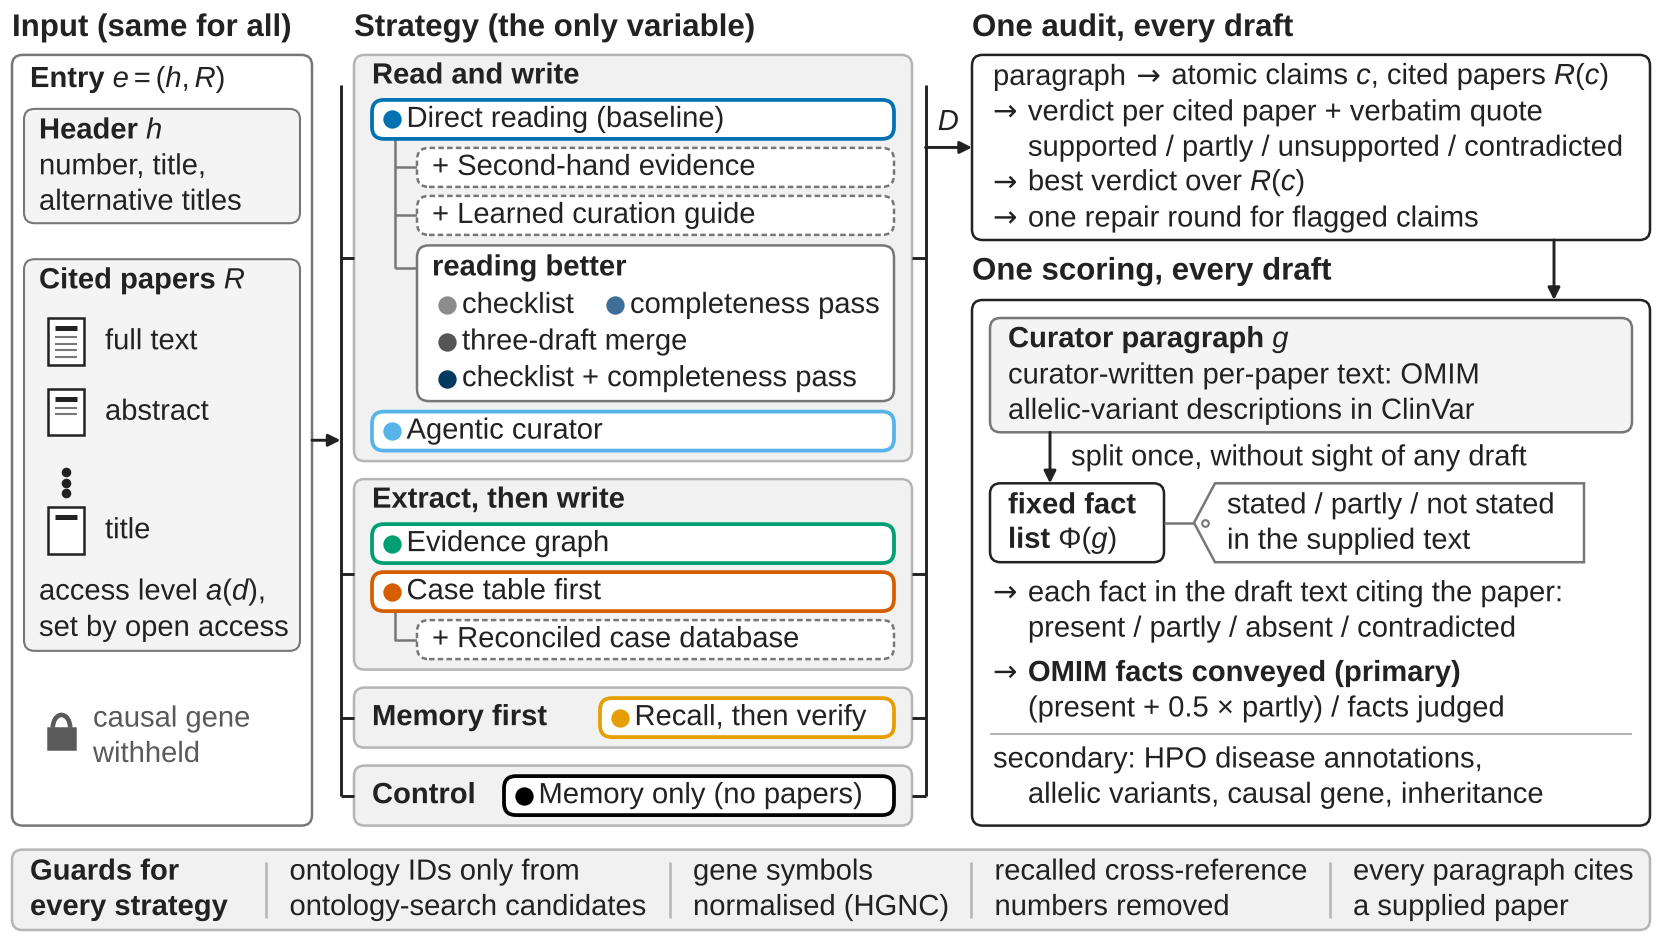
\includegraphics[width=\linewidth]{figures/fig_overview.png}
\end{center}
\caption{Benchmark overview. Every strategy receives an entry $e=(h,R)$: its header and exactly the papers the curators cited, each readable as full text, abstract or title by open access. Only the strategy varies (add-ons dashed under their parent; reading-better arms tested on entries with full text not used in their design). Flagged claims get one repair round, except in the control and the reading-better arms. Scoring uses curator text about the cited papers, not whole entries. Main set: 100 entries; 515 papers (96 full text, 345 abstract, 74 title); 476 curator paragraphs; 6,652 fixed facts.}
\label{fig:overview}
\end{figure}

\textbf{Access to the source bounds agreement in the regime tested.} This is expected, as curators read full papers; we measure its size. Hiding the full text of papers that have one lowers coverage of the same facts from 79.8\% to 36.1\% (means over 46 entries, all before the audit's repair round; $+43.7$ points, 95\% CI $+38.3$ to $+49.1$). \textbf{No design beat direct reading in the regime tested.} For entries with 2--12 references read in one prompt, at the main settings and on the 93 entries every strategy finished, no design conveyed more than direct reading: the agent and the evidence graph were 0.6 and 0.5 points behind (intervals $-1.3$ to $+0.0$ and $-1.5$ to $+0.5$; no equivalence is claimed) and our case-table implementation 1.9 points ($-3.1$ to $-0.8$), a suggestive deficit. The graph was ahead only on subsets of entries (the 30 replicate entries; the 38 of a post hoc ablation), and matching settings narrowed the case table's gap by 2.1 points; each difference is small against the effect of full text. \textbf{Reading more completely recovers a few points and writes more.} On 38 entries not used in its design, each with a complete draft from every arm, a completeness pass adds 2.6 points (1.7 to 3.6), with drafts of 14,412 instead of 10,802 characters; on all 41 (post hoc) the gain holds only if the unrevised draft is kept where the model's safety filter stopped the revision ($+2.4$ points; $-3.5$ if such entries count as zero). \textbf{The audit checks fidelity, not completeness or correctness.} It caught every planted citation swap but no added citation and, by construction, no omission.

We contribute (1) a benchmark harness built only from public resources \citep{sayers2026database,Louden2020MedgenNcbis,rosonovski2024europe,seal2023genenames}, releasing every draft, verdict and score per entry but not the curator text; (2) a controlled comparison of the paradigms, with completion under safety-filter stops, run-to-run variation, a matched ablation and a memory-only control by creation date; (3) a within-paper measurement of the effect of access and of the gain from reading better; and (4) a map of the audit's blind spots, all under one model family whose judgements no person validated.
%%%%%%%%% INTRODUCTION %%%%%%%%%

\section{Related Work}
\label{sec:related_work}
%%%%%%%%% RELATED WORK %%%%%%%%%
\paragraph{Language models for curation in genetics and biology.}
Language models assist the curation of knowledge bases, ontologies, gene and gene-set annotations and literature summaries \citep{caufield2024structured,caufield2024curategpt,toro2024dynamic,Li2025GenewhispererEnhancing,hu2025evaluation,niyonkuru2025leveraging,Green2026GoflowllmcuratingMirna,Murphy2024HarnessingGenerative,Green2023LitsummLarge}, and extract variant, gene--disease and gene--phenotype evidence from papers \citep{li2025autopm3,furlan2025eagleai,wang2026pubmind,yin2026benchmarking,twede2026evidence}. Model recall of curated rare-disease knowledge is generally low, better for genes than phenotypes \citep{groza2026systematic}, and GEN-KnowRD builds a knowledge base from model-generated profiles, evaluated by disease ranking \citep{yan2026genknowrd}. Closest to ours, FlyAOC compares memorisation, pipeline and agent harnesses that recover FlyBase curators' annotations given a 16,898-paper corpus \citep{zhang2026flyaoc}. Two benchmarks built from ClinGen judge model explanations or summaries against human-written ones, comparing models, not strategies \citep{queen2025cgbench,Saadat2026LargeLanguage}; PaperQA2's cited Wikipedia-style summaries are compared with Wikipedia articles \citep{skarlinski2024language}; and agents given a source publication annotate phenotypes within inter-curator variability \citep{balhoff2026frontier}. Here the papers are fixed to the curators' reference list, the reference is the curators' own per-paper text and fields, access is manipulated within the same papers, and the strategy is the only variable; the contribution is this controlled measurement, not a new strategy.

\paragraph{Intermediate representations versus long-context reading.}
Whether long-context reading beats retrieval is contested \citep{Li2024LongContext,Yu2024DefenseRag,liu2024lost,Zhang2024ChainAgents,Li2025LaraBenchmarking}. Graphs serve query-focused summarisation \citep{edge2024local}, and comparisons ask when they help \citep{han2025rag,xiang2025use}; retrieval-augmented systems write cited answers \citep{Lla2023PaperqaRetrievalaugmented,Asai2024OpenscholarSynthesizing,singh2025ai2}, and STORM writes Wikipedia-like articles \citep{shao2024assisting}.

\paragraph{Memory, verification and contamination.}
Verification methods plan verification questions \citep{dhuliawala2024chainofverification}, post-edit unsupported content \citep{Gao2022RarrResearching} or consult domain databases \citep{wang2025geneagent}. As curated knowledge bases are public, memory is a confound; contamination is detected from black-box access \citep{Shi2023DetectingPretraining,oren2024proving,golchin2024time,Golchin2025DataContamination} or with training cut-offs and new test items \citep{Roberts2023DataContamination,Jain2024LivecodebenchHolistic,White2024LivebenchChallenging}. We read a memory-only control by creation date, including entries created in 2026.

\paragraph{Improving a fixed reader.}
Prompts are optimised by models \citep{Zhou2022LargeLanguage,Pryzant2023AutomaticPrompt,Yang2023LargeLanguage}, evolved \citep{Guo2023EvopromptConnecting,Fernando2023PromptbreederSelfreferential,agrawal2026gepa} or compiled \citep{Khattab2023DspyCompiling,Opsahlong2024OptimizingInstructions}; self-refinement helps \citep{Madaan2023SelfrefineIterative} but can fail without feedback \citep{Huang2023LargeLanguage}, and the most consistent sample helps \citep{Wang2022SelfconsistencyImproves,Chen2023UniversalSelfconsistency}. Our guide and reading-better arms are small prompt-level instances.

\paragraph{Evaluating cited long-form text.}
Factuality metrics check atomic claims against a knowledge source \citep{min2023factscore,wei2024longform,Song2024VeriscoreEvaluating}, and human evaluation checks attribution to identified sources \citep{Rashkin2021MeasuringAttribution}. Citation support is often incomplete in generative search, cited generation and medical answers \citep{Liu2023EvaluatingVerifiability,gao2023enabling,wu2025automated}, and about a quarter of quotations in medical articles are erroneous \citep{jergas2015quotation}. Model judges can match human preferences \citep{zheng2023judging} but need validation \citep{shankar2024who} and may favour their own outputs \citep{panickssery2024llm}; a model reviewing extracted data caught 2 of 39 deliberate errors \citep{Stewartevans2025ExpeditingData}. Our judges share the writer's model family.
%%%%%%%%% RELATED WORK %%%%%%%%%

\section{Benchmark and Strategies}
\label{sec:method}
%%%%%%%%% METHOD %%%%%%%%%
\subsection{Task, entries and reference}
\label{sec:task}
An entry is $e=(h,R)$ with header $h$ (number, title, alternative titles) and references $R=\{d_1,\dots,d_n\}$, the papers its curators cited. Each paper has an access level $a(d)\in\{\text{full text},\text{abstract},\text{title}\}$ set by open access. A strategy $S$ maps $(h,R)$ to a draft $D$: paragraphs, each citing a non-empty subset of $R$, and sets of genes, inheritance modes, ontology terms and allelic variants. The causal gene is withheld, as naming it is part of the curator's task.

\textbf{Entries.} We drew 100 OMIM phenotype entries at random with a fixed seed, 20 from each of five bands of entry number that track creation date (1xxxxx--5xxxxx, 600000--609999, 610000--615999, 616000--619999, 620000 onward). Eligible entries have 2--12 cited references, a causal gene in the gene map, at least five phenotype annotations and at least one curator paragraph in scope; this selects well-annotated, molecularly characterised entries. Of the 515 cited papers, 96 (19\%) are readable in full through PubMed Central or Europe PMC \citep{rosonovski2024europe}, 345 as abstract only and 74 as title only; supplements were not retrieved. Appendix Table~\ref{tab:app_experiments} lists the entries of every experiment.

\textbf{Reference.} The \emph{curator-written per-paper text} is OMIM's allelic-variant descriptions as deposited by OMIM in ClinVar \citep{landrum2025clinvar}: variant-centred prose from OMIM's gene entries, each paragraph about one or more cited papers. A paragraph is in scope when it is about a paper its entry cites; 476 are. Of the 515 cited papers, 327 have an in-scope paragraph (81 of 96 readable in full, 221 of 345 abstract only, 25 of 74 title only); what a draft says about the other papers is not scored. Narrative sections of phenotype entries are not public and are not compared. The clinical-synopsis reference is the HPO disease annotations \citep{gargano2024human}: 2,311, of which 1,835 are the HPO team's own curation from papers and 476 are taken from OMIM. The causal gene comes from OMIM's gene map via MedGen \citep{Louden2020MedgenNcbis} and mim2gene; inheritance from HPO and MedGen modes, compared as coarse classes that must be equal as sets; the variants are the 427 in-scope OMIM-submitted ClinVar records.

\textbf{Reuse.} The fixed fact lists contain curator wording and are not redistributed, so scoring a new strategy against the same denominators requires rebuilding the reference under the rights holder's terms and splitting it again. How much a fresh split by the same procedure moves levels was not measured; splitting afresh for each draft, a different procedure, ran 2--5 points higher with the same order of strategies (Appendix Table~\ref{tab:app_full}). Differences within one split are the comparable quantity.

\subsection{Strategies and settings}
\label{sec:strategies}
The strategies form three paradigms, a control and three add-ons, each add-on tested against its parent (Figure~\ref{fig:overview}; Appendix Table~\ref{tab:app_strategies}). \emph{Read and write}: \textbf{direct reading}, the baseline, puts all papers in one prompt; the \textbf{agentic curator} works in a folder of the papers with read and search tools and must give a verbatim quote for every paragraph. \emph{Extract, then write}: the \textbf{evidence graph} extracts quote-backed findings per paper into a graph of papers, genes, variants, phenotypes and inheritance; \textbf{case table first} extracts one record per reported patient or family per paper and pools them; in both, the writer sees only the intermediate. \emph{Memory first}: \textbf{recall, then verify} writes from memory, audits the draft against the papers and keeps, restates, corrects or deletes claims; as its writer adds nothing from the papers, it is no competitor on coverage but shows how much of what memory supplies survives verification. The \textbf{memory-only control} is the memory draft with no papers, audited but not repaired. The four strategies that read the papers are the \emph{reading strategies}. The add-ons are \textbf{second-hand evidence} on direct reading (passages from later open-access papers that describe a paper not readable in full), a \textbf{reconciled case database} on case table first and a \textbf{learned curation guide} on direct reading (two reflection rounds on 27 training entries).

\textbf{Settings and guards.} One model, Claude Opus 5.5, writes, extracts, audits and judges through a command-line interface with schema-constrained output and no temperature or seed. Writers run at high reasoning effort. \emph{In the main comparison, per-paper extraction in the evidence graph and the case table runs at medium effort, and their synopsis terms (and the case table's inheritance) are assigned by rule}; the audit and all judging also run at medium effort. A matched ablation raises extraction to high effort and lets the writer choose synopsis terms (Section~\ref{sec:main}). For every strategy, ontology identifiers come only from ontology-search candidates, gene symbols are normalised against HGNC \citep{seal2023genenames}, recalled entry cross-reference numbers are removed, and every paragraph must cite a supplied paper; no strategy has web access, and replies are cached.

\subsection{Definitions, audit, scoring and statistics}
\label{sec:scoring}
\textbf{Definitions.} Each in-scope curator paragraph $g$ was split once, without sight of any draft, into a fixed list $\Phi(g)$ of atomic \emph{facts}, reused for every strategy. A judge marks each fact \emph{present} (conveyed), \emph{partly present} (conveyed less precisely), absent or contradicted in what draft $D$ says in its paragraphs citing $g$'s papers. Over an entry's facts, \emph{coverage} is $\mathrm{cov}(D)=(\#\text{present}+\tfrac12\,\#\text{partly present})/\#\text{facts judged}$, and \emph{OMIM facts conveyed}, the primary endpoint, is $\mathrm{cov}(D)$ averaged over entries. A level is a \emph{mean over entries} unless marked \emph{pooled} (one ratio over all facts of a group); paired differences are always means over entries. A fact is \emph{stated} in the supplied text when the judge gives a quote for it that is found verbatim in the text available for its paper, and otherwise \emph{partly stated} or \emph{not stated}; this is a property of the text, the same for every strategy. A \emph{stopped reply} is one the model's safety filter ended: it comes back empty, is recorded and is never retried with a changed prompt, and its reasons are not visible. A strategy \emph{completes} an entry when it writes a draft with every paper processed. A stopped reply costs a one-call strategy the whole entry but a per-paper strategy one paper, so under the \emph{symmetric rule} strategies are compared only on entries every compared strategy completed, and completion is reported as an outcome. A draft is \emph{repaired} after the audit's one repair round and \emph{unrepaired} before it; a comparison is \emph{like for like} when its arms share the same entries and the same repair state. \emph{Held out}: the entries created in 2026 from all development; the reading-better test split from the design of its prompts and from guide learning, not from the development of the main strategies.

\textbf{Audit.} Each paragraph is split into atomic claims $c$ attributed to the papers $R(c)\subseteq R$ it cites. Each cited paper gives a verdict $v(c,d)\in\{$supported, partly supported, unsupported, contradicted$\}$ with a quote; a ``supported'' verdict whose quote is not verbatim in the paper is downgraded. A claim takes the best verdict over $R(c)$ (Section~\ref{sec:audit} shows what this hides), and flagged claims (unsupported or contradicted) get one repair round. \emph{Judged supported} means a final verdict of ``supported'', a judgement of fidelity to the cited text. Unsupported is not wrong, so unsupported and contradicted are reported separately.

\textbf{Secondary measures} (Appendix~\ref{app:settings}): synopsis HPO terms (F1; exact, hierarchical, Lin similarity; \citealp{Khler2009ClinicalDiagnostics,Resnik1995UsingInformation}), allelic variants (recall; precision, counting a variant OMIM does not list as a miss), causal-gene F1 and inheritance agreement; predicting nothing where the reference is non-empty scores zero. The primary endpoint has no length or precision counterpart, so it rewards recall; we report draft length beside coverage gains.

\textbf{Statistics.} Paired differences from direct reading come with a percentile bootstrap 95\% interval over entries (10,000 resamples; \citealp{Efron1979BootstrapMethods}), entries better/worse/tied and an exact two-sided sign test with ties dropped \citep{Dixon1946StatisticalSign}. Sign tests on the eight secondary headline measures are Holm-adjusted within each strategy \citep{holm1979simple}; the primary endpoint is not adjusted across the five comparisons with direct reading. The interval over entries is the test of a difference; run-to-run noise, from three replicates of generation, audit and scoring on 30 entries, is a yardstick, not a test. ``Points'' are percentage points.

\textbf{Status of each analysis} (Appendix Table~\ref{tab:app_experiments}). \emph{Pre-specified}: the main comparison on the primary endpoint over the symmetric set, the hidden-full-text experiment, and the first three reading-better arms against their baseline. \emph{Choices made after results were seen}: (a) fixed fact lists replaced splitting afresh for each draft; (b) the symmetric rule, adopted after a first analysis had put the evidence graph 2.1 points below direct reading (Appendix~\ref{app:corrected}); (c) the matched ablation; (d) the restrictions by what the supplied text states, and the provenance of conveyed facts; (e) scoring the hidden-full-text arm before repair; (f) re-auditing planted-test paragraphs unaltered; (g) a claim-selection rule for deleted qualifiers widened after the run; (h) the fourth reading-better arm, designed after the other arms' held-out results were seen; (i) the reading-better analysis with stopped entries put back. (a) and (b) apply to every result; (c)--(i) are marked \emph{post hoc}. \emph{Exploratory}: groupings across entries, runs on 10 or fewer entries, and planted errors at 30 items per class. The rest is \emph{secondary}.
%%%%%%%%% METHOD %%%%%%%%%

\section{Experiments}
\label{sec:experiments}
%%%%%%%%% EXPERIMENTS %%%%%%%%%
Results are pre-specified or secondary unless marked post hoc or exploratory (Section~\ref{sec:scoring}).

\subsection{Access to the source bounds agreement}
\label{sec:access}
\begin{figure}[t]
\begin{center}
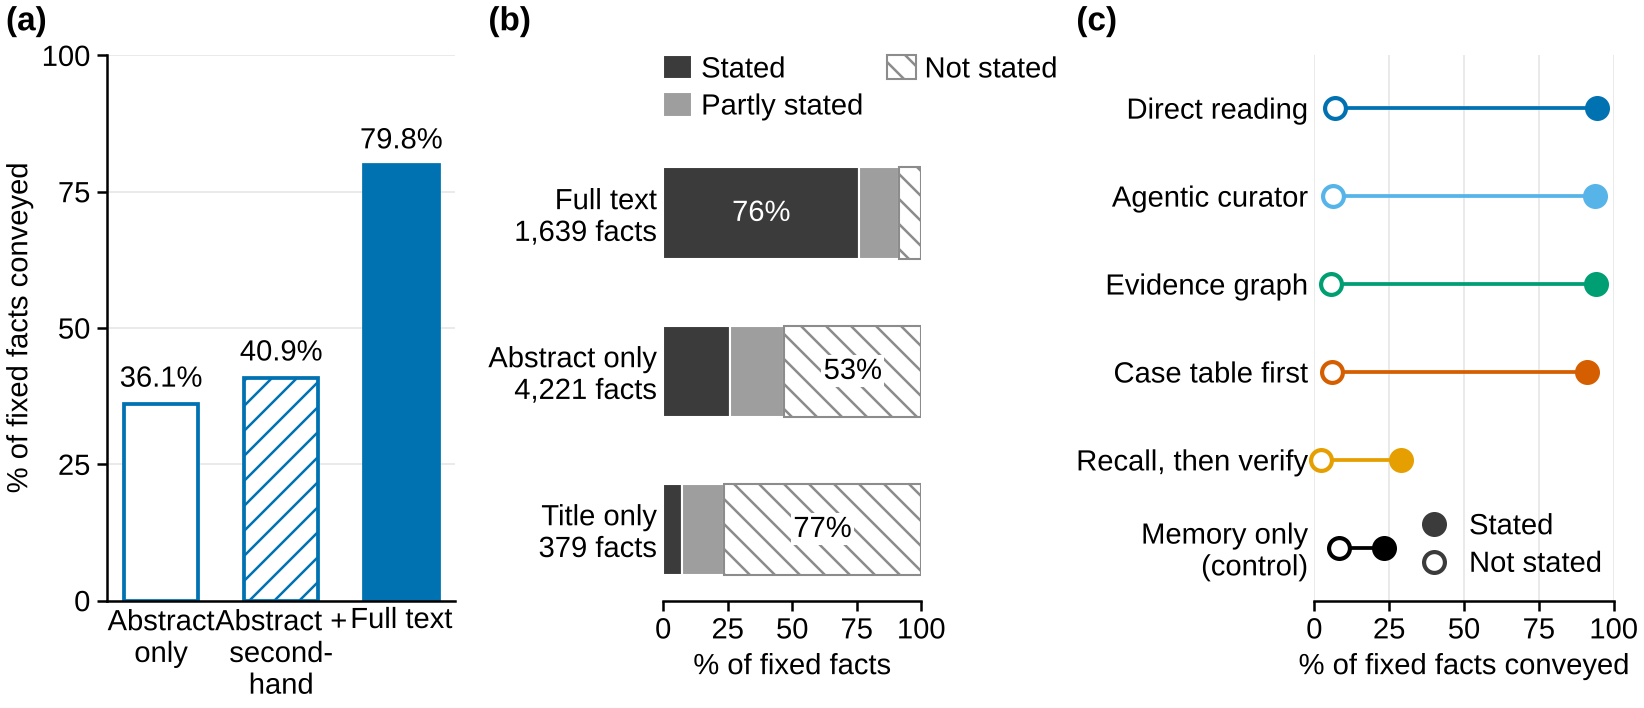
\includegraphics[width=\linewidth]{figures/fig_access_bound.png}
\end{center}
\caption{Access bounds what a strategy can convey. (a) Hidden full text: OMIM facts conveyed by direct reading on the same 46 entries and the 2,120 fixed facts of every in-scope paragraph about a hidden paper, with the papers readable in full given as abstract, abstract plus second-hand passages, or full text (means over entries; every arm unrepaired). (b) Whether the supplied text states the 6,239 fixed facts of the 93 compared entries (\% of row, pooled). (c) Coverage of facts the text states (filled; 89 entries) and does not state (hollow; 90), means over entries. Panels (b) and (c) are post hoc; ``stated'' is a model judgement that needs a verified quote.}
\label{fig:access}
\end{figure}

\textbf{Hiding the full text of the same papers.} The experiment used the 49 entries with a full-text paper that an in-scope curator paragraph is about and hid all 91 of their full-text papers (the other 5 have no in-scope paragraph, so hiding them could not change the score). Each entry was rewritten by direct reading from the abstracts, with and without second-hand passages; 46 have a full-text draft (the writer was stopped on 3). The facts scored are those of every in-scope paragraph about a hidden paper: 136 paragraphs, 2,120 facts. The by-access tables class a paragraph about several papers by its least readable paper, so 283 of these facts count as abstract or title only there. Like for like, with every arm unrepaired (a post hoc rescoring of the full-text drafts before repair), full text conveys 43.7 points more than the abstracts alone ($+38.3$ to $+49.1$; Figure~\ref{fig:access}a), better on 45 entries and tied on one. Repairing the full-text arm, as first designed, moves it by 0.2 points (Appendix Table~\ref{tab:app_hidden}). Coverage by access level across different papers (Appendix Table~\ref{tab:app_access}) is observational and confounded with creation date and journal.

\textbf{Second-hand passages substitute only in part.} For the same hidden papers, passages from later open-access papers that describe them add 4.9 points to the abstracts ($+2.8$ to $+7.1$); as an add-on on 96 entries they add 1.8 points ($+1.0$ to $+2.8$) but raise the share of claims unsupported before repair, and of 112 claims about hidden papers resting on a passage, the full text leaves 11 unsupported (an upper bound, as supplements were excluded) and contradicts 3 (Appendix~\ref{app:hidden}).

\textbf{What the supplied text states} (post hoc). The supplied text states three quarters of the facts about full-text papers but only a quarter of those about abstract-only papers (pooled; Figure~\ref{fig:access}b). The reading strategies convey 91.0--94.4\% of the facts the text states and 5.5--6.9\% of those it does not (Figure~\ref{fig:access}c); on the latter they do no better than the memory-only control (8.2\%). This contrast agrees with the hidden-full-text result but holds partly by construction: ``stated'' needs a quote the model found, so facts that need inference are more likely classed as not stated. On facts stated in abstract-only papers most entries tie, so this restriction has a ceiling of its own (Appendix Table~\ref{tab:app_stated}).

\textbf{Missed and conveyed facts} (direct reading, 97 entries, pooled). The text states 49\% of the facts not fully conveyed from full-text papers (Appendix Figure~\ref{fig:missed}); over all facts, 4\% were not fully conveyed although stated, the headroom for reading better. Of facts conveyed in full from abstract-only papers, 24 of 1,420 (1.7\%) are stated in no supplied text, and of those conveyed in part, 58 of 583 (10.0\%; post hoc): recalled, inferred or misjudged, which the analysis does not separate.

\subsection{Strategies under one control}
\label{sec:main}
\begin{table}[t]
\caption{Main comparison at the main settings: 93 of 100 entries every strategy completed (means over entries). Facts: OMIM facts conveyed (primary, \%). $\Delta$: paired difference from direct reading in points, bootstrap 95\% interval, entries better/worse/tied (---: not applicable, the baseline). Claims: audited claims per entry. Secondary (\%): claims judged supported (after repair; memory only is unrepaired), synopsis HPO F1 (exact), variant precision, causal-gene F1. Price: generation list price per entry. Subscripts: entries, if fewer than 93. Matched ablation: Appendix Table~\ref{tab:app_abl_main}.}
\label{tab:main}
\begin{center}
\footnotesize
\setlength{\tabcolsep}{2.6pt}
\begin{tabular}{@{}lrlrrrrrr@{}}
\toprule
Strategy & Facts & $\Delta$ facts (95\% CI); b/w/t & Claims & Supp. & HPO F1 & Var.\ prec. & Gene & Price \\
\midrule
Direct reading & 49.1 & --- & 101.0 & 96.1 & 35.9 & 88.7$_{82}$ & 97.5 & \$0.26 \\
Agentic curator & 48.4 & $-0.6$ ($-1.3$, $+0.0$); 31/42/20 & 97.3 & 96.4 & 35.6 & 87.9$_{82}$ & 97.5 & \$0.28 \\
\midrule
Evidence graph & 48.6 & $-0.5$ ($-1.5$, $+0.5$); 33/45/15 & 113.5 & 96.5 & 34.6 & 76.9$_{87}$ & 98.2 & \$0.56 \\
Case table first & 47.2 & $-1.9$ ($-3.1$, $-0.8$); 31/48/14 & 117.9 & 94.7 & 34.0 & 72.9$_{88}$ & 93.9 & \$0.61 \\
\midrule
Recall, then verify & 14.6 & $-34.5$ ($-39.2$, $-29.9$); 2/89/2 & 26.3 & 94.2$_{92}$ & 24.9 & 100.0$_{23}$ & 82.8 & \$0.70 \\
\midrule
Memory only & 15.1 & $-34.0$ ($-39.3$, $-28.7$); 7/85/1 & 28.2 & 50.8 & 30.6 & 97.2$_{30}$ & 83.9 & \$0.07 \\
\bottomrule
\end{tabular}
\end{center}
\end{table}

\textbf{At the main settings the agent and the evidence graph are not distinguishable from direct reading} (Table~\ref{tab:main}; completion in Appendix Table~\ref{tab:app_completion}). They trail it by 0.6 and 0.5 points (sign tests $p=0.242$ and $0.213$). No secondary measure differs after Holm adjustment (Appendix Table~\ref{tab:app_sign}). No margin was set in advance, so this is no equivalence claim. As a yardstick, replicate noise gives a 95\% half-width of 1.0 point on such a difference over 93 entries (Appendix~\ref{app:stability}). Counting a missing draft as zero on all 100 entries turns the agent's difference to $+0.4$ ($-1.0$ to $+2.7$; Appendix Table~\ref{tab:app_itt}). The extract-then-write drafts say more (113.5 and 117.9 audited claims per entry against 101.0), which a recall endpoint does not penalise.

\textbf{The case table's deficit is suggestive.} Our case-table implementation trails direct reading by 1.9 points ($-3.1$ to $-0.8$). Its sign test does not reach 0.05 ($p=0.071$), the five comparisons with direct reading are not adjusted, and counting missing drafts as zero gives an interval that includes zero. Restricted to facts stated in full-text papers (post hoc), the gap is 8.4 points ($-14.3$ to $-3.8$; 40 entries; Figure~\ref{fig:design}a). The case table also writes more variants that OMIM does not list (130 against 36, pooled).

\textbf{Settings and entry sets} (post hoc; Appendix~\ref{app:ablation}). A matched ablation reran the extract-then-write strategies with per-paper extraction at high effort and writer-chosen synopsis terms on 38 entries chosen with more full text, reusing the main run's drafts otherwise. There, at the main settings, the evidence graph was already 1.0 point above direct reading ($-0.9$ to $+2.8$) and the case table 2.3 below (Appendix Table~\ref{tab:app_abl_main}). Matching moved the case table by $+2.1$ points ($+1.1$ to $+3.2$; 25 entries better, 8 worse) but the evidence graph by only $+0.8$ ($-0.5$ to $+2.1$); as both changes were made together, crediting effort is an inference. The clear settings effect is the case table's; the evidence graph's sign depends on the entries averaged ($-1.2$ points on the ablation's 19 entries with half or more full text, $+3.1$ on the other 19, same drafts). Which design is ahead thus depends on the entries and, for the case table, on settings.

\textbf{Memory first and contamination.} Recall, then verify keeps 14.6\% coverage (memory draft 15.1\%) while the share of claims judged supported rises from 50.8\% to 94.2\%. Memory alone conveys 24.1\% of facts in the 600000--609999 band, 5.7\% in the newest band and 7.0\% on 20 compared entries created in 2026 (five strategies ran on 30; stopped replies were frequent). There no strategy conveyed more than direct reading, and the agent's and the case table's intervals exclude zero (Appendix~\ref{app:new}; Figure~\ref{fig:memory}). From the header alone, memory names the causal gene with an F1 of 88.9--100\% in the four older bands but 41.2\% from 620000 on (Appendix Table~\ref{tab:app_era}). Reading is not shown free of memorisation (exploratory). On abstract-only papers, direct reading's pooled coverage by band, oldest to newest (33.0, 49.8, 42.0, 40.2, 37.9\%), moves with the memory-only control's (12.8, 22.9, 14.0, 10.8, 6.0\%; Appendix Table~\ref{tab:app_era_access}). This is consistent with recall contributing to abstract-only coverage but does not separate recall from reading. Direct reading's mean coverage is lowest in the oldest band (34.9\%, against 51.2--53.9\%), which we did not analyse.

\textbf{Two add-ons} (Appendix~\ref{app:addons}). The learned guide did not improve its own training entries and adds 1.0 point ($+0.0$ to $+2.0$) on 68 held-out entries; this says nothing about stronger prompt optimisation. Reconciliation moved no score by more than 0.1 point; its case database is unvalidated.

\subsection{Reading better within what access allows}
\label{sec:better}
\begin{figure}[t]
\begin{center}
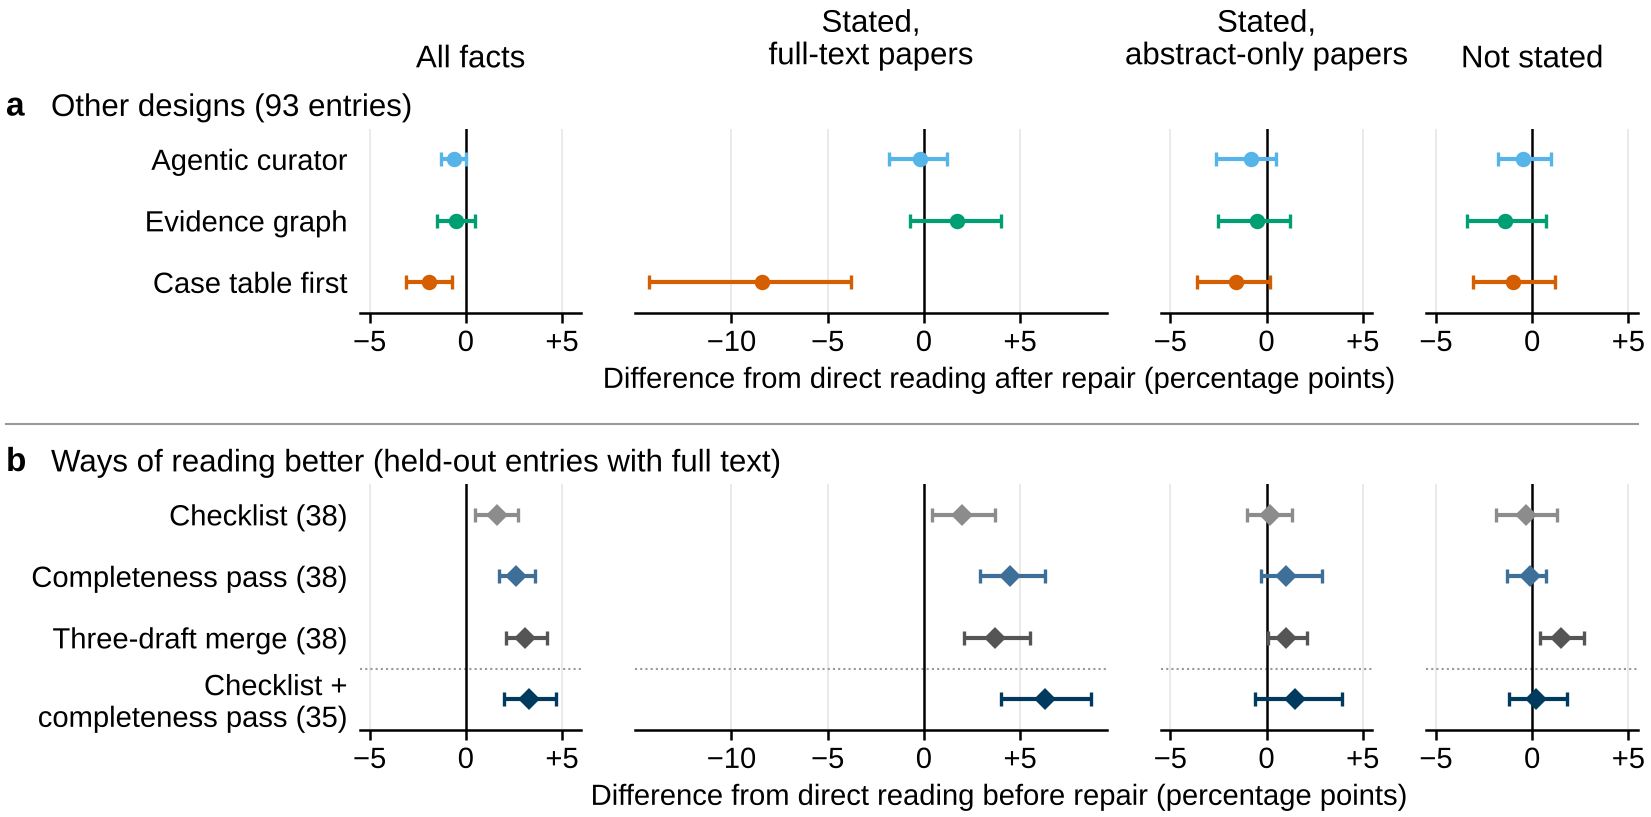
\includegraphics[width=\linewidth]{figures/fig_design_vs_reading.png}
\end{center}
\caption{Paired differences in OMIM facts conveyed (points; mean and bootstrap 95\% interval over entries) on all facts, on facts the supplied text states (in full-text or abstract-only papers) and on facts it does not state (a model judgement; these restrictions are post hoc). (a) Other designs minus direct reading at the main settings, after repair, 93 entries (40, 79 and 90 in the restrictions). Memory-based strategies are off scale. (b) Held-out entries with full text: reading better minus direct reading's draft, all unrepaired (entries in parentheses; 34, 31 and 36 in the restrictions, or 32, 28 and 33 for the post hoc combined arm).}
\label{fig:design}
\end{figure}

Half of what direct reading misses in full-text papers is stated in their text, and the audit cannot see omissions. Of ten approaches reviewed, we tested three variants of direct reading. Their prompts were written on three training entries and frozen before the 41 held-out entries with a paper readable in full were run. A \textbf{checklist} lists what a curator records about each paper. In a \textbf{completeness pass}, a per-paper check lists findings the paper states but the draft omits, each with a quote verified in the paper, and one revision adds only those. A \textbf{three-draft merge} keeps every distinct statement. A fourth arm, the \textbf{checklist with the completeness pass}, was designed after the other arms' held-out results were seen and run on the same entries (post hoc). No arm is repaired; the baseline is direct reading's unrepaired draft. The first three arms are compared on the 38 entries all completed (Holm-adjusted across the three), the fourth on the 35 all five completed (Appendix~\ref{app:better}).

\textbf{A completeness pass recovers facts the text states, and writes more.} It adds 2.6 points ($+1.7$ to $+3.6$; 28/4/6; Holm-adjusted $p<0.001$), and its drafts are longer: 14,412 characters per entry against 10,802, and 164 checkable claims per audited entry against 129. The gain lies on facts the supplied text states, most of it on full-text papers ($+4.5$, $+2.9$ to $+6.3$; Figure~\ref{fig:design}b); coverage of facts the text does not state does not change. The only precision-side check, the share of claims judged supported, did not fall on the 20 audited entries (97.2\% against 97.0\%; no interval; Appendix Table~\ref{tab:app_better_claims}).

\textbf{Stopped revisions} (post hoc). The completeness pass lacked a complete draft on 3 of the 41 entries and the combined arm on 6 (4 without a draft); direct reading completed all 41. Keeping all 41, and scoring the draft a stopped revision would have revised (as the adopted default does), the completeness pass conveys 2.4 points more than direct reading ($+1.5$ to $+3.4$) and the combined arm 3.1 ($+1.8$ to $+4.3$; 32/7/2). Counting such an entry as zero, both fall below direct reading on the mean ($-3.5$ and $-4.8$; intervals including zero), though each is better on more entries than worse (Appendix Table~\ref{tab:app_better_itt}). The gain thus depends on keeping the unrevised draft.

\textbf{The checklist, the combined arm and the merge.} The checklist adds 1.6 points ($+0.5$ to $+2.7$; 11,837 characters per entry), with Holm-adjusted $p=0.058$. The combined arm adds 3.3 points ($+2.0$ to $+4.7$; 35 entries; 14,963 characters against 10,826), only 0.8 more than the completeness pass ($-0.4$ to $+1.8$): the two overlap. The merge adds 3.1 points ($+2.1$ to $+4.2$; 14,245 characters), partly on facts the text does not state, with more unsupported and contradicted claims and lower variant precision (83.4\% against 87.1\%): merging brings in content the papers do not support.

\textbf{Scope and cost.} No arm was tested on entries without full text; on facts stated in abstract-only papers no arm moved coverage by more than 1.5 points. The gains are of the size the headroom allowed, far below what full text adds, at \$2.10 and \$2.11 per entry from scratch for the completeness arms against \$1.09. The lever with the largest expected effect, reading papers free to read but not openly licensed (about a third of curator facts concern them), was not tested.

\subsection{Exploratory runs on 10 or fewer entries}
\label{sec:released}
\textbf{Released pipelines.} PaperQA2's document-query pipeline without its agent \citep{skarlinski2024language}, GraphRAG with local search \citep{edge2024local} and STORM \citep{shao2024assisting}, which produced no article, ran at one setting each on the same papers and model (Appendix~\ref{app:released}; 10 and 4 entries). \textbf{Input size.} Six entries were padded with unrelated full-text papers to about 500,000 and 1,200,000 characters; no draft cited an added paper, so this tests size, not crowding (Appendix~\ref{app:padding}). On the 2 entries every strategy completed at every size, direct reading changed by $+4.7$ and $+3.5$ points, the others by $-3.0$ to $+2.1$. On 6 entries allowing stopped calls on added papers, direct reading rose 3.6 points ($+1.0$ to $+5.9$) at about 500,000 characters and the others moved at most 1.0, leaving them 2.8--4.6 points further behind (interaction intervals exclude zero, sign tests do not reach 0.05; not at 1,200,000). Unpadded drafts are an earlier generation, so changes mix size with run-to-run variation. \textbf{Large entries.} On four new entries with 76--148 references, the safety filter stopped at least one strategy on every entry (Appendix~\ref{app:large_new}). \textbf{30--75 references.} Ten compared entries, mostly abstracts, give no findings (Appendix~\ref{app:tier}). Each run shows directions and large effects only.

\subsection{What the audit can and cannot see}
\label{sec:audit}
\begin{figure}[t]
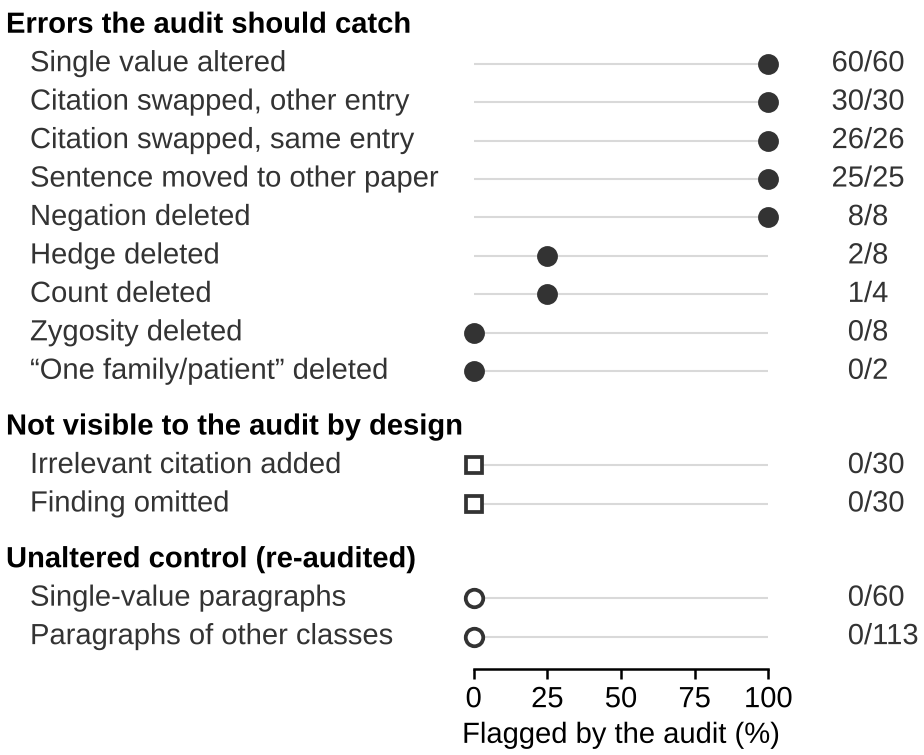
\includegraphics[width=0.55\linewidth]{figures/fig_audit_coverage.png}\hfill
\begin{minipage}[b]{0.42\linewidth}
\caption{Planted errors the audit flagged (flagged/total at right, items whose truth is known): a planted claim judged unsupported or contradicted (for omissions and controls, any claim). Single value: an earlier test; other rows: six classes of 30 items (exploratory), the five ``deleted'' rows being rules of one class. All were planted in evidence-graph paragraphs the audit had passed; the controls had passed once, so they give no false-flag rate. No row is a sensitivity estimate.}
\label{fig:audit}
\end{minipage}
\end{figure}

\textbf{What it removes and catches.} Unrepaired, the memory-only control has 22.1\% of claims unsupported; the repaired reading strategies keep 94.7--96.5\% judged supported. A single value altered by rule (count, zygosity, residue or mode of inheritance) in 60 paragraphs the audit had passed was flagged every time, and none of the 60 was flagged when re-audited unaltered (post hoc; Figure~\ref{fig:audit}): blunt single-value substitutions are caught, which is not a sensitivity estimate. Of six further classes of 30 items each (exploratory), citation swaps to another entry's paper or within the entry and variant sentences moved between papers' paragraphs were caught wherever truth is known (30/30, 26/26, 25/25), but swaps are easy: the swapped paper is usually off-topic. The deleted-qualifier class was caught in 11 of 30 items: all 8 deleted negations (2 only under a claim-selection rule widened after the run), but 2 of 8 hedges, 1 of 4 counts and none of 8 zygosity or 2 ``one family'' deletions (Appendix~\ref{app:audit}).

\textbf{What it misses.} An added irrelevant citation is invisible because a claim takes the best verdict over its cited papers: none of 30 was flagged, although the added paper's own verdict was ``unsupported'' for all 176 claims attributed to it. In real multi-citation paragraphs of the reading strategies, 4--7\% of (claim, cited paper) pairs are judged not to support the claim (entries changed by repair excluded). Omissions are invisible by construction; a completeness check by the same model listed 16 of 29 planted deletions in full and none in the unaltered texts. The audit checks fidelity, not correctness: a copied source error passes, as does a claim resting only on a later paper's passage.

\section{Discussion, Limitations and Conclusion}
\label{sec:discussion}
For one model, entries with 2--12 references whose papers fit one prompt, and 19\% of papers readable in full, access to the source limits agreement with curator-written variant facts far more than how a strategy reads. The regime favours direct reading (most papers are abstracts; 2,669 of 6,239 compared facts are not stated in the supplied text; stated full-text facts span 40 entries), yet the same measurement resolved gains of a few points from reading better. \textbf{Measurement lessons:} treat stopped replies symmetrically; fix fact lists before scoring; split coverage by what the text states; report run-to-run noise and draft length beside intervals; compare designs on the same entries and settings before crediting the representation; keep per-paper audit verdicts; check that released pipelines run with the intended model.

\textbf{Limitations, and what each missing check would establish.} (i) No person has validated any judgement, all made by one model family. Expert labels on a stratified sample, with chance-corrected agreement, would establish whether the levels, strategy differences, stated/not-stated contrast and audit catches hold (95.7\% agreement between two judgings shows only self-consistency); differences of a few points are the most exposed to judge error, and a manual check of facts classed as not stated would show how much of that contrast is mechanical. (ii) No second model family was run: a judge from another family would test self-preference and correlated errors between the ``stated'' and ``conveyed'' judgements, and a second writer whether the access effect and the order of strategies transfer, notably to smaller-context models. The same model's safety filter removed entries unevenly across strategies for reasons not visible, so comparisons on completed entries condition on an outcome of the strategy. (iii) Entries with few references dominate: input size was tested only by padding with unrelated text, and large sets of relevant papers, where designs might separate, could not be compared (stopped replies); matched settings ran on 38 entries, and each paradigm has one implementation. With no margin set in advance, parity is untested; an equivalence analysis against a pre-set margin would test it. (iv) The endpoint rewards recall, with no length or precision counterpart; a length-matched baseline or length-controlled endpoint would show how much of the reading-better gains exceeds writing more. (v) The reference is indirect and narrow (variant-centred paragraphs, ontology annotations from two sources, gene and inheritance tables): about 24\% of a direct-reading draft's statements have a counterpart in it (Appendix~\ref{app:addons}), so most draft content is checked only by the audit; the fact lists are not redistributed, and a fresh split's stability is unmeasured. (vi) Every strategy is given the curators' reference list; finding the literature was tested on ten entries (Appendix~\ref{app:updates}). (vii) Only open-access text without supplements was used, where much variant and patient data lives. (viii) Variant names are not validated against reference sequences; inheritance is compared as coarse classes. (ix) The main strategies were developed on their evaluation entries; held-out evidence is limited to the 2026 entries and the reading-better arms. (x) Each entry was run once, without temperature or seed control; cost is at list price. (xi) The audit misses over-citation, most broadened claims and omissions; a larger stress test would give per-class sensitivity, and an any-cited-paper-fails rule applied to stored verdicts its flag rate. (xii) Released systems ran at one setting each, PaperQA2 without its agent, STORM not at all; intended runs would test them as released, and direct reading through the six questions would separate protocol from design.
%%%%%%%%% EXPERIMENTS %%%%%%%%%

%%%%%%%%% CONCLUSION %%%%%%%%%
\textbf{Conclusion.} Hiding the full text of the same papers lowers coverage of curator-written variant facts from 79.8\% to 36.1\%. For entries with 2--12 references read in one prompt, no other design conveyed more than direct reading at the main settings; which comes closest depends on entries and settings. The audit checks fidelity, not completeness; no person validated any judgement.
%%%%%%%%% CONCLUSION %%%%%%%%%

\section*{Ethics Statement}
The benchmark is built from public resources (NCBI, ClinVar, HPO, MedGen, Europe PMC, HGNC). Curator-written text is used for scoring and is not redistributed; released score files carry fact identifiers and statuses, not wording. Whether others can rebuild the reference and score against the same fact lists depends on the rights holders' terms of use for curated text, which apply to anyone who does so. No human subjects were involved. Generated entries are drafts for expert review and are not clinical guidance; they must be marked as machine generated and not as OMIM content. A passed audit is not a check of correctness or completeness: it passes a draft that faithfully copies a source's error and does not detect omissions or over-citation, so an expert who trusts an audited draft may miss both. No curator has checked any draft, and disagreements between drafts and the reference reported here are unconfirmed.

\section*{Reproducibility Statement}
Section~\ref{sec:method} specifies the entry sampling (fixed seed, five creation-era bands, eligibility rules), the reference sources, the strategies, settings, guards, audit, scoring, statistics and the status of each analysis; Appendix Table~\ref{tab:app_experiments} gives the entry set and status of every experiment, Appendix~\ref{app:settings} the model settings, and Appendix~\ref{app:released} the released systems' versions, entry points and every setting changed from their defaults. One model (Claude Opus 5.5) was used through a command-line interface that exposes no temperature or seed, so exact regeneration is not guaranteed; we report replicate and judge variation instead (Appendix~\ref{app:stability}). Replies are cached, so each call was made once; all experiments, pilots and re-scoring used 45,291 cached model calls, 338 million input and 82 million output tokens, about \$3,587 at list price. The curator-written text and the fixed fact lists are not redistributed; every part of the reference can be rebuilt from public resources under the rights holders' terms, but a rebuilt reference must be split again, and differences are comparable within one split. The harness and the per-entry drafts, verdicts and scores are released as supplementary material. After the evaluation, the released harness writes entries with the checklist and completeness pass by default where a paper is readable in full, keeping the unrevised draft when the revision is stopped; this is a project decision, not a finding of the study.

%%%%%%%%% REFERENCES %%%%%%%%%
\bibliography{references}
\bibliographystyle{iclr2025_conference}
%%%%%%%%% REFERENCES %%%%%%%%%

%%%%%%%%% Appendix %%%%%%%%%
\clearpage
\appendix
\setlength{\belowcaptionskip}{4pt}
\makeatletter
\setlength{\@fptop}{0pt}
\setlength{\@fpbot}{0pt plus 1fil}
\setlength{\@fpsep}{8pt plus 2pt minus 2pt}
\setlength{\abovecaptionskip}{4pt}
\setlength{\intextsep}{8pt plus 2pt minus 2pt}
\setlength{\floatsep}{8pt plus 2pt minus 2pt}
\setlength{\textfloatsep}{12pt plus 2pt minus 2pt}
\makeatother
\FloatBarrier
\section{Experiments and entry sets}
\label{app:experiments}
\begin{table}[!htbp]
\caption{Every experiment, its status (Section~\ref{sec:scoring}), its entry set, the entries compared and why others dropped out. Status: \emph{pre-specified}; \emph{post hoc}, chosen after results were seen (Section~\ref{sec:scoring} lists every such choice); \emph{exploratory}, 10 or fewer entries, 30 planted items per class, or observational groupings; \emph{secondary}, the other analyses. ``Stopped'': a reply was stopped by the model's safety filter (no draft if it was the writer's); ``per-paper call failed'': a per-paper call was lost (incomplete draft). Entries are compared only when every strategy in the comparison completed them.}
\label{tab:app_experiments}
\scriptsize
\begin{tabularx}{\linewidth}{>{\raggedright\arraybackslash}p{2.5cm}>{\raggedright\arraybackslash}p{1.3cm}>{\raggedright\arraybackslash}p{2.6cm}>{\centering\arraybackslash}p{1.0cm}>{\raggedright\arraybackslash}X>{\raggedright\arraybackslash}p{1.2cm}}
\toprule
Experiment & Status & Entry set & Com\-pared & Why entries dropped out & Where \\
\midrule
Main comparison (six strategies) & Pre-specified & 100 main entries (2--12 references, five creation-era bands) & 93 & 7 entries: no draft (direct reading 3, agentic curator 2, evidence graph 1); per-paper call failed (evidence graph 3, case table first 3) & Sec.~\ref{sec:main}, App.~\ref{app:main} \\
Missing drafts counted as zero & Secondary (sensitivity) & 100 main entries & 100 & none; missing drafts scored zero & App.~\ref{app:main} \\
Groups by access (observational) & Exploratory & the 93 compared entries & 46 / 25 / 21 & the one entry with all references readable in full is in no group & App.~\ref{app:access} \\
Facts the supplied text states & Post hoc & the 93 compared entries & 89 / 40 / 79 / 90 & an entry counts in a restriction only if it has facts there (stated / stated, full-text papers / stated, abstract-only papers / not stated) & Sec.~\ref{sec:access}, App.~\ref{app:access} \\
Missed-fact attribution; conveyed-fact provenance & Secondary; provenance post hoc & 100 main entries, direct reading & 97 & 3 without a draft (writer stopped) & Sec.~\ref{sec:access}, App.~\ref{app:access} \\
Hidden full text & Pre-specified; scoring the full-text arm before repair post hoc & 49 main entries with a full-text paper that an in-scope paragraph is about (all their 91 full-text papers hidden) & 46 & 3 whose full-text direct-reading draft was stopped & Sec.~\ref{sec:access}, App.~\ref{app:hidden} \\
Judge variation; run-to-run replicates & Secondary & 30-entry replicate subset (six per band) & 30 & none & App.~\ref{app:stability} \\
Matched ablation & Post hoc & 40 entries weighted towards full text & 38 & high-effort extraction stopped (graph variants 1 entry each, table variants 2 each) & Sec.~\ref{sec:main}, App.~\ref{app:ablation} \\
Second-hand evidence (add-on) & Secondary & 100 main entries & 96 & not completed by both strategies & Sec.~\ref{sec:access}, App.~\ref{app:hidden} \\
Reconciled case database & Secondary & 100 main entries & 97 & not completed by both strategies & Sec.~\ref{sec:main}, App.~\ref{app:addons} \\
Learned curation guide & Secondary & 70 held-out main entries (guide learned on 27 of 30 training entries) & 68 & not completed by both strategies & Sec.~\ref{sec:main}, App.~\ref{app:addons} \\
Reading better (four arms; five arms) & Pre-specified (first three arms); fourth arm post hoc & 41 held-out entries with at least one paper readable in full & 38 / 35 & stopped: completeness pass 3 entries (no draft); checklist with completeness pass 6 (4 no draft, 2 incomplete) & Sec.~\ref{sec:better}, App.~\ref{app:better} \\
Reading better, every entry with stopped entries put back & Post hoc & the same 41 entries & 41 & none; a lost entry is counted as zero or replaced by the draft the stopped revision would have revised & Sec.~\ref{sec:better}, App.~\ref{app:better} \\
Reading better, audit without repair & Secondary & a seeded sample of 20 of the 41 & 20 & none (stopped audit calls leave claims not checkable) & Sec.~\ref{sec:better}, App.~\ref{app:better} \\
Entries created June--November 2026 (five strategies) & Secondary; held out from all development & 30 newest of 53 eligible 2026 entries, chosen by creation date alone & 20 & stopped (agentic curator 6, direct reading 2); per-paper call failed (evidence graph 7, case table first 10) & Sec.~\ref{sec:main}, App.~\ref{app:new} \\
\bottomrule
\end{tabularx}
\end{table}

\begin{table}[!htbp]
\caption{Every experiment, continued: the exploratory runs and checks (columns as in Table~\ref{tab:app_experiments}).}
\label{tab:app_experiments2}
\scriptsize
\begin{tabularx}{\linewidth}{>{\raggedright\arraybackslash}p{2.5cm}>{\raggedright\arraybackslash}p{1.3cm}>{\raggedright\arraybackslash}p{2.6cm}>{\centering\arraybackslash}p{1.0cm}>{\raggedright\arraybackslash}X>{\raggedright\arraybackslash}p{1.2cm}}
\toprule
Experiment & Status & Entry set & Com\-pared & Why entries dropped out & Where \\
\midrule
30--75 references & Exploratory & 12 entries & 10 & 2 entries: no draft (direct reading 1, evidence graph 1); per-paper call failed (case table first, both) & Sec.~\ref{sec:released}, App.~\ref{app:tier} \\
Released systems & Exploratory & first 10 entries of a seeded order; GraphRAG the first 4 within its call budget & 10 / 4 / 0 & GraphRAG: the fifth entry did not fit the call budget; STORM: every chain-of-thought prompt of its research stage stopped & Sec.~\ref{sec:released}, App.~\ref{app:released} \\
Padding of the input & Exploratory & 6 ablation entries with at least half their papers readable in full & 6 / 2 & stopped extraction calls on added papers (allowed in the 6-entry analysis; the symmetric rule leaves 2) & Sec.~\ref{sec:released}, App.~\ref{app:padding} \\
Large entries & Exploratory & 4 new entries with 76--148 references & 0 & every entry: no draft (direct reading 3, agentic curator 2, case table first 1) or papers stopped (evidence graph 4 entries, case table first 3) & Sec.~\ref{sec:released}, App.~\ref{app:large_new} \\
Planted single values; unaltered re-audit & Secondary; re-audit post hoc & 60 paragraphs the audit had passed & 60 & none (in the re-audit, 3 of 361 claims could not be audited) & Sec.~\ref{sec:audit}, App.~\ref{app:audit} \\
Planted errors, six further classes & Exploratory; claim selection for deleted qualifiers widened post hoc & 30 items per class in evidence-graph paragraphs the audit had passed; 113 unaltered paragraphs as controls & 30 / 26 / 25 / 30 / 30 / 30 & truth not known by construction: 4 same-entry swaps, 5 moved sentences & Sec.~\ref{sec:audit}, App.~\ref{app:audit} \\
Completeness check & Exploratory & 30 planted deletions and the same texts unaltered; 60 natural omissions on 28 papers & 29 / 60 & one item stopped (both its texts) & Sec.~\ref{sec:audit}, App.~\ref{app:audit} \\
Citation precision (stored audits) & Exploratory & multi-citation paragraphs of the main run & 78--100 per strategy & entries whose paragraphs the repair round changed (per-paper verdicts not recoverable) & Sec.~\ref{sec:audit}, App.~\ref{app:audit} \\
Draft--reference disagreements & Exploratory & 37 facts a direct-reading draft contradicted & 37 & none & App.~\ref{app:updates} \\
Updates; retrieval without a reference list & Exploratory & 10 entries each (evidence graph only) & 10 & none & App.~\ref{app:updates} \\
\bottomrule
\end{tabularx}
\end{table}

\FloatBarrier
\section{Strategies, model settings and guards}
\label{app:settings}
Table~\ref{tab:app_strategies} describes each strategy. Settings: one model for everything, Claude Opus 5.5 (\texttt{claude-opus-5-5}), called through the Claude Code command-line interface in headless mode with schema-constrained output; no temperature or seed is exposed. Reasoning effort is high for writers (direct reading, the graph and table writers, the agent, the memory draft) and medium for per-paper extraction in the evidence graph and case table first, for the audit and for all judging; the matched ablation raises per-paper extraction to high. The agentic strategy has read and search tools over a folder of the papers and nothing else. The agentic curator reports which papers it opened (self-reported; tool calls are not logged): in the 98 entries it wrote it reported opening every paper, and all 2,600 quotes it gave were found verbatim in the papers. The memory drafts that recall, then verify starts from are the memory-only control's drafts. The evidence graph discards any finding whose quote is not in the paper (none was). Synopsis terms are assigned by a lexical search over the ontology's labels and synonyms that returns candidates, from which the model chooses. Secondary measures: synopsis terms are compared with the HPO annotations exactly, hierarchically (both sets expanded with all ancestors) and by Lin semantic similarity, an ontology-aware comparison in the spirit of \citet{Khler2009ClinicalDiagnostics}; Lin similarity uses information content computed from the ontology's disease annotations, averaged in each direction to give precision and recall. Allelic variants are matched on normalised protein or nucleotide change, with a model judge for names that do not normalise; precision counts a variant OMIM does not list as a miss whether or not the paper reports it. No fact went unjudged in any run.

\begin{table}[!htbp]
\caption{The strategies: three paradigms, a control, three add-ons each tested against its parent, and the four ways of reading better (variants of direct reading, Section~\ref{sec:better}). Guards for every strategy: ontology identifiers chosen only from ontology-search candidates; gene symbols normalised against HGNC; entry cross-reference numbers recalled from memory removed; every paragraph must cite a supplied paper.}
\label{tab:app_strategies}
\scriptsize
\begin{tabularx}{\linewidth}{>{\raggedright\arraybackslash}p{2.4cm}>{\raggedright\arraybackslash}p{2.6cm}>{\raggedright\arraybackslash}X}
\toprule
Strategy & Paradigm & What it does \\
\midrule
Direct reading & Read and write & All papers in one prompt; the model writes the entry. Baseline. \\
Agentic curator & Read and write & The model works in a folder of the papers with read and search tools and must give a verbatim quote for every paragraph. \\
Evidence graph & Extract, then write & Quote-backed findings are extracted per paper (findings whose quote is not in the paper are discarded) and joined into a graph of papers, genes, variants, phenotypes and inheritance; the writer sees only the graph. Synopsis terms are computed from the graph by rule; inheritance is written by the writer. \\
Case table first & Extract, then write & One record per reported patient or family is extracted per paper and pooled; synopsis terms and inheritance are computed by rule, candidate genes are confirmed by the writer; the writer sees only the table. \\
Recall, then verify & Memory first & The model writes from memory; the draft is audited against the papers; a rewriter keeps supported claims, restates partly supported ones, corrects contradicted ones and deletes the rest. It may not add content from the papers. \\
Memory only & Control & The memory draft, with no papers. Audited, not repaired. \\
Second-hand evidence & Add-on to direct reading & For a paper not readable in full, passages from later open-access papers that cite and describe it are added, marked as second-hand, for the writer and the audit. \\
Reconciled case database & Add-on to case table first & A propose, verify, apply step merges the same patient, family or variant reported in several papers and settles conflicts. \\
Learned curation guide & Add-on to direct reading & A guide of general rules, learned in two reflection rounds from 27 training entries' omissions and extras, is appended to the writer's prompt; tested on 70 held-out entries. \\
Checklist & Reading better & Direct reading with a curator checklist in the house style: what a curator records about each paper. \\
Completeness pass & Reading better & For each paper, a check lists findings the paper states that the draft omits, each with a quote verified in the paper; one revision then adds only those. \\
Three-draft merge & Reading better & Three direct-reading drafts merged, keeping every distinct statement. \\
Checklist with completeness pass & Reading better & The checklist draft followed by the completeness pass; designed after the other arms had run. \\
\bottomrule
\end{tabularx}
\end{table}

\FloatBarrier
\section{Main comparison: full results}
\label{app:main}
Counting only facts conveyed in full (row ``fully'' of Table~\ref{tab:app_full}) lowers every level and keeps the order of strategies; paired differences under full credit only are not reported for the restrictions by what the text states. Extract-then-write raises synopsis recall at lower precision and produces more variants OMIM does not list (Tables~\ref{tab:app_full} and~\ref{tab:app_varinh}). At list price, read-and-write costs \$1.15--\$1.18 per entry in all and extract-then-write \$1.72--\$1.78 (Table~\ref{tab:app_cost}). The paired differences of Table~\ref{tab:app_paired} and those restricted by what the supplied text states (Table~\ref{tab:app_stated}) come from two bootstrap runs and can differ in the last digit of an interval bound; each table keeps its own.
\begin{table}[!htbp]
\caption{Completion on the 100 main entries. An entry is compared only when every strategy completed it in full; 93 qualify (left out: 118210, 300148, 609296, 617232, 620609, 621030, 621068).}
\label{tab:app_completion}
\scriptsize
\begin{tabularx}{\linewidth}{>{\raggedright\arraybackslash}p{2.4cm}>{\centering\arraybackslash}p{1.0cm}>{\centering\arraybackslash}X>{\centering\arraybackslash}p{2.9cm}}
\toprule
Strategy & Complete & Incomplete (a per-paper call failed) & No draft \\
\midrule
Evidence graph & 96 & 3: 118210 (1 paper), 617232 (1 paper), 621030 (1 paper) & 1: 620609 \\
Direct reading & 97 & 0 & 3: 609296, 620609, 621068 \\
Agentic curator & 98 & 0 & 2: 609296, 620609 \\
Memory only (control) & 100 & 0 & 0 \\
Recall, then verify & 100 & 0 & 0 \\
Case table first & 97 & 3: 300148 (1 paper), 617232 (2 papers), 621068 (1 paper) & 0 \\
\bottomrule
\end{tabularx}
\end{table}

\begin{table}[!htbp]
\caption{All measures, means over the 93 compared entries ($\uparrow$ higher is better, $\downarrow$ lower is better). The primary endpoint is OMIM facts conveyed; the others are secondary. The row ``facts split afresh for each draft'' is the earlier scoring, which runs 2--5 points higher and gives the same ordering. The memory-only control is audited but never repaired, so its before-repair rows are as audited.}
\label{tab:app_full}
\scriptsize
\begin{tabularx}{\linewidth}{>{\raggedright\arraybackslash}p{4.2cm}>{\centering\arraybackslash}X>{\centering\arraybackslash}X>{\centering\arraybackslash}X>{\centering\arraybackslash}X>{\centering\arraybackslash}X>{\centering\arraybackslash}X}
\toprule
Metric & Evidence graph & Direct reading & Agentic curator & Memory only (control) & Recall, then verify & Case table first \\
\midrule
Claims judged supported by cited paper $\uparrow$ & 96.5\% & 96.1\% & 96.4\% & 50.8\% & 94.2\% (n=92) & 94.7\% \\
\ldots{} unsupported, before the repair round $\downarrow$ & 0.2\% & 0.2\% & 0.1\% & 22.1\% & 0.6\% (n=92) & 0.3\% \\
\ldots{} contradicted, before the repair round $\downarrow$ & 0.1\% & 0.0\% & 0.0\% & 0.6\% & 0.1\% (n=92) & 0.0\% \\
OMIM per-paper facts conveyed (primary endpoint) $\uparrow$ & 48.6\% & 49.1\% & 48.4\% & 15.1\% & 14.6\% & 47.2\% \\
\ldots{} fully (no partial credit) $\uparrow$ & 42.0\% & 42.4\% & 41.9\% & 10.2\% & 10.1\% & 40.8\% \\
OMIM per-paper facts contradicted $\downarrow$ & 0.4\% & 0.4\% & 0.4\% & 0.5\% & 0.3\% & 0.5\% \\
\ldots{} facts split afresh for each draft (earlier scoring) $\uparrow$ & 51.5\% & 52.1\% & 51.3\% & 20.4\% & 18.2\% & 49.3\% \\
Clinical synopsis HPO F1, exact $\uparrow$ & 34.6\% & 35.9\% & 35.6\% & 30.6\% & 24.9\% & 34.0\% \\
\ldots{} precision $\uparrow$ & 40.6\% & 44.1\% & 45.5\% & 53.5\% (n=92) & 53.6\% (n=87) & 40.7\% \\
\ldots{} recall $\uparrow$ & 37.4\% & 36.2\% & 34.2\% & 24.1\% & 18.4\% & 37.7\% \\
Clinical synopsis HPO F1, hierarchical $\uparrow$ & 54.7\% & 56.1\% & 56.2\% & 48.2\% & 40.5\% & 53.7\% \\
OMIM allelic variants recovered $\uparrow$ & 65.9\% & 66.5\% & 65.9\% & 15.2\% & 11.6\% & 64.3\% \\
Generated variants that are OMIM variants (precision) $\uparrow$ & 76.9\% (n=87) & 88.7\% (n=82) & 87.9\% (n=82) & 97.2\% (n=30) & 100.0\% (n=23) & 72.9\% (n=88) \\
Causal gene F1 $\uparrow$ & 98.2\% & 97.5\% & 97.5\% & 83.9\% & 82.8\% & 93.9\% \\
\ldots{} recall $\uparrow$ & 98.4\% & 97.3\% & 97.3\% & 83.9\% & 82.8\% & 94.1\% \\
Inheritance matches OMIM $\uparrow$ & 92.5\% & 93.5\% & 93.5\% & 82.8\% & 73.1\% & 91.4\% \\
OMIM references used $\uparrow$ & 94.6\% & 94.4\% & 93.3\% & 33.6\% & 65.2\% & 94.6\% \\
\bottomrule
\end{tabularx}
\vspace{4pt}
\begin{tabularx}{\linewidth}{>{\raggedright\arraybackslash}p{4.2cm}>{\centering\arraybackslash}X>{\centering\arraybackslash}X>{\centering\arraybackslash}X>{\centering\arraybackslash}X>{\centering\arraybackslash}X>{\centering\arraybackslash}X}
\toprule
Metric & Evidence graph & Direct reading & Agentic curator & Memory only (control) & Recall, then verify & Case table first \\
\midrule
Claims audited per entry & 113.5 & 101.0 & 97.3 & 28.2 & 26.3 & 117.9 \\
Claims that could not be audited per entry & 1.2 & 0.6 & 0.3 & 0.0 & 0.0 & 0.4 \\
Clinical-synopsis HPO terms per entry & 19.2 & 15.4 & 13.8 & 6.2 & 4.4 & 21.0 \\
Allelic variants per entry & 3.9 & 3.2 & 3.2 & 0.4 & 0.3 & 4.1 \\
\bottomrule
\end{tabularx}
\end{table}

\begin{table}[!htbp]
\caption{Paired differences from direct reading on the 93 compared entries: points (means over entries), bootstrap 95\% interval, entries better/worse/same. Sign tests and Holm-adjusted results are in Table~\ref{tab:app_sign}.}
\label{tab:app_paired}
\scriptsize
\begin{tabularx}{\linewidth}{>{\raggedright\arraybackslash}p{3.0cm}>{\centering\arraybackslash}X>{\centering\arraybackslash}X>{\centering\arraybackslash}X>{\centering\arraybackslash}X>{\centering\arraybackslash}X}
\toprule
Metric & Evidence graph & Agentic curator & Memory only (control) & Recall, then verify & Case table first \\
\midrule
Claims judged supported by cited paper $\uparrow$ & +0.4 ($-$0.4 to +1.3); 41/45/7 & +0.3 ($-$0.4 to +1.0); 53/33/7 & $-$45.3 ($-$50.3 to $-$40.3); 2/90/1 & $-$1.9 ($-$3.5 to $-$0.4); 34/53/5 (n=92) & $-$1.4 ($-$2.7 to $-$0.4); 34/56/3 \\
\ldots{} unsupported, before the repair round $\downarrow$ & +0.0 ($-$0.3 to +0.2); 10/12/71 & $-$0.1 ($-$0.4 to +0.1); 11/8/74 & +22.4 (+18.3 to +26.7); 1/79/13 & +0.4 ($-$0.0 to +0.9); 10/10/72 (n=92) & +0.1 ($-$0.2 to +0.4); 12/18/63 \\
OMIM per-paper facts conveyed (primary) $\uparrow$ & $-$0.5 ($-$1.5 to +0.5); 33/45/15 & $-$0.6 ($-$1.3 to +0.0); 31/42/20 & $-$34.0 ($-$39.3 to $-$28.7); 7/85/1 & $-$34.5 ($-$39.2 to $-$29.9); 2/89/2 & $-$1.9 ($-$3.1 to $-$0.8); 31/48/14 \\
OMIM per-paper facts contradicted $\downarrow$ & +0.0 ($-$0.1 to +0.2); 8/5/80 & +0.0 ($-$0.1 to +0.2); 3/5/85 & +0.1 ($-$0.2 to +0.5); 17/14/62 & $-$0.1 ($-$0.2 to +0.2); 16/7/70 & +0.1 ($-$0.1 to +0.3); 5/8/80 \\
Clinical synopsis HPO F1, exact $\uparrow$ & $-$1.3 ($-$3.3 to +0.6); 34/45/14 & $-$0.3 ($-$1.5 to +0.8); 38/32/23 & $-$5.3 ($-$9.2 to $-$1.5); 41/52/0 & $-$11.0 ($-$14.4 to $-$7.6); 25/63/5 & $-$2.0 ($-$3.9 to $-$0.1); 39/45/9 \\
Clinical synopsis HPO F1, hierarchical $\uparrow$ & $-$1.4 ($-$2.8 to $-$0.1); 36/44/13 & +0.0 ($-$1.0 to +1.1); 40/35/18 & $-$7.9 ($-$12.3 to $-$3.5); 38/54/1 & $-$15.7 ($-$19.9 to $-$11.5); 21/68/4 & $-$2.5 ($-$4.1 to $-$0.9); 34/51/8 \\
OMIM allelic variants recovered $\uparrow$ & $-$0.5 ($-$3.1 to +2.5); 4/8/81 & $-$0.6 ($-$2.2 to +0.7); 3/3/87 & $-$51.3 ($-$60.0 to $-$42.4); 3/69/21 & $-$54.9 ($-$62.8 to $-$47.0); 0/71/22 & $-$2.2 ($-$4.9 to +0.3); 6/11/76 \\
Causal gene F1 $\uparrow$ & +0.7 (+0.0 to +2.1); 1/0/92 & +0.0 (+0.0 to +0.0); 0/0/93 & $-$13.6 ($-$21.5 to $-$6.1); 2/15/76 & $-$14.7 ($-$22.6 to $-$7.5); 1/15/77 & $-$3.6 ($-$8.6 to +0.4); 1/4/88 \\
Inheritance matches OMIM $\uparrow$ & $-$1.1 ($-$5.4 to +2.1); 1/2/90 & +0.0 ($-$3.2 to +3.2); 1/1/91 & $-$10.8 ($-$19.4 to $-$2.1); 3/13/77 & $-$20.4 ($-$29.0 to $-$11.8); 1/20/72 & $-$2.1 ($-$8.6 to +4.3); 4/6/83 \\
\bottomrule
\end{tabularx}
\end{table}

\begin{table}[!htbp]
\caption{Sign tests on the 93 compared entries: exact two-sided sign test on the paired differences from direct reading (ties dropped). The primary endpoint is not adjusted. For the secondary headline measures the sign-test $p$-value was adjusted by Holm's method across those measures within each strategy; the last column lists the measures whose adjusted $p$ is below 0.05, with adjusted $p$ and the mean paired difference in points.}
\label{tab:app_sign}
\scriptsize
\begin{tabularx}{\linewidth}{>{\raggedright\arraybackslash}p{2.4cm}>{\centering\arraybackslash}p{2.6cm}>{\centering\arraybackslash}p{1.4cm}>{\raggedright\arraybackslash}X}
\toprule
Strategy minus direct reading & Primary endpoint: sign test $p$ (better / worse / tied) & Secondary headline measures & \ldots{} with Holm-adjusted $p<0.05$ \\
\midrule
Evidence graph & 0.213 (33 / 45 / 15) & 8 & none \\
Agentic curator & 0.242 (31 / 42 / 20) & 8 & none \\
Memory only (control) & $<$0.001 (7 / 85 / 1) & 8 & Claims supported by cited paper ($<$0.001; $-$45.3); claims unsupported or contradicted, before the repair round ($<$0.001; +22.4); OMIM allelic variants recovered ($<$0.001; $-$51.3); causal gene F1 (0.011; $-$13.6) \\
Recall, then verify & $<$0.001 (2 / 89 / 2) & 8 & Clinical synopsis HPO F1, exact ($<$0.001; $-$11.0); clinical synopsis HPO F1, hierarchical ($<$0.001; $-$15.7); OMIM allelic variants recovered ($<$0.001; $-$54.9); causal gene F1 (0.002; $-$14.7); inheritance matches OMIM ($<$0.001; $-$20.4) \\
Case table first & 0.071 (31 / 48 / 14) & 8 & none \\
\bottomrule
\end{tabularx}
\end{table}

\begin{table}[!htbp]
\caption{Pooled counts of audited claims and OMIM facts on the 93 compared entries.}
\label{tab:app_pooled}
\scriptsize
\begin{tabularx}{\linewidth}{>{\raggedright\arraybackslash}p{3.4cm}>{\centering\arraybackslash}X>{\centering\arraybackslash}X>{\centering\arraybackslash}X>{\centering\arraybackslash}X>{\centering\arraybackslash}X>{\centering\arraybackslash}X}
\toprule
 & Evidence graph & Direct reading & Agentic curator & Memory only (control) & Recall, then verify & Case table first \\
\midrule
Claims audited & 10,552 & 9,390 & 9,051 & 2,624 & 2,448 & 10,969 \\
\ldots{} supported & 10,227 & 9,069 & 8,802 & 1,343 & 2,308 & 10,497 \\
\ldots{} partly supported & 325 & 321 & 248 & 687 & 140 & 472 \\
\ldots{} unsupported & 0 & 0 & 1 & 576 & 0 & 0 \\
\ldots{} contradicted & 0 & 0 & 0 & 18 & 0 & 0 \\
Claims audited before repair & 10,526 & 9,371 & 9,056 & 2,624 & 2,448 & 10,945 \\
\ldots{} unsupported before repair & 20 & 17 & 10 & 576 & 13 & 21 \\
\ldots{} contradicted before repair & 8 & 0 & 2 & 18 & 4 & 4 \\
OMIM facts scored & 6,239 & 6,239 & 6,239 & 6,239 & 6,239 & 6,239 \\
\ldots{} conveyed & 2,562 & 2,620 & 2,593 & 502 & 502 & 2,490 \\
\ldots{} partly conveyed & 811 & 820 & 796 & 578 & 553 & 769 \\
\ldots{} missing & 2,840 & 2,771 & 2,820 & 5,133 & 5,167 & 2,948 \\
\ldots{} contradicted & 26 & 28 & 30 & 26 & 17 & 32 \\
\bottomrule
\end{tabularx}
\end{table}

\begin{table}[!htbp]
\caption{Allelic-variant precision (pooled) and inheritance errors by kind on the 93 compared entries. Precision counts a variant OMIM does not list as a miss whether or not the paper reports it.}
\label{tab:app_varinh}
\scriptsize
\begin{tabularx}{\linewidth}{>{\raggedright\arraybackslash}p{3.8cm}>{\centering\arraybackslash}X>{\centering\arraybackslash}X>{\centering\arraybackslash}X>{\centering\arraybackslash}X>{\centering\arraybackslash}X>{\centering\arraybackslash}X}
\toprule
 & Evidence graph & Direct reading & Agentic curator & Memory only (control) & Recall, then verify & Case table first \\
\midrule
Variants generated & 365 & 295 & 300 & 40 & 28 & 381 \\
\ldots{} matching an OMIM variant of the entry & 253 & 258 & 259 & 38 & 28 & 250 \\
\ldots{} listed by OMIM only from a paper outside the entry's references & 1 & 1 & 1 & 1 & 0 & 1 \\
\ldots{} not in OMIM & 111 & 36 & 40 & 1 & 0 & 130 \\
Pooled precision (entries where OMIM lists variants) & 69.3\% & 87.5\% & 86.3\% & 95.0\% & 100.0\% & 65.6\% \\
\bottomrule
\end{tabularx}
\vspace{4pt}
\begin{tabularx}{\linewidth}{>{\raggedright\arraybackslash}p{3.8cm}>{\centering\arraybackslash}X>{\centering\arraybackslash}X>{\centering\arraybackslash}X>{\centering\arraybackslash}X>{\centering\arraybackslash}X>{\centering\arraybackslash}X}
\toprule
 & Evidence graph & Direct reading & Agentic curator & Memory only (control) & Recall, then verify & Case table first \\
\midrule
Entries with an OMIM mode of inheritance & 93 & 93 & 93 & 93 & 93 & 93 \\
\ldots{} matched & 86 & 87 & 87 & 77 & 68 & 85 \\
\ldots{} none stated & 3 & 2 & 3 & 13 & 22 & 2 \\
\ldots{} a mode missing & 0 & 0 & 0 & 0 & 0 & 1 \\
\ldots{} an extra mode & 3 & 4 & 3 & 1 & 1 & 4 \\
\ldots{} a different mode & 1 & 0 & 0 & 2 & 2 & 1 \\
\bottomrule
\end{tabularx}
\end{table}

\begin{sidewaystable}
\caption{Sensitivity analysis (intention to treat): all 100 entries, a missing draft counted as zero on each higher-is-better measure with a reference; incomplete drafts kept as scored; lower-is-better measures averaged over existing drafts. Missing drafts: evidence graph 1, direct reading 3, agentic curator 2. Bottom: paired differences from direct reading with interval, median, better/worse/tie and exact sign-test $p$.}
\label{tab:app_itt}
\scriptsize
\begin{tabularx}{\linewidth}{>{\raggedright\arraybackslash}p{4.4cm}>{\centering\arraybackslash}X>{\centering\arraybackslash}X>{\centering\arraybackslash}X>{\centering\arraybackslash}X>{\centering\arraybackslash}X>{\centering\arraybackslash}X}
\toprule
Metric & Evidence graph & Direct reading & Agentic curator & Memory only (control) & Recall, then verify & Case table first \\
\midrule
Claims judged supported by cited paper $\uparrow$ & 95.7\% & 93.2\% & 94.5\% (n=99) & 51.5\% & 94.4\% (n=98) & 94.5\% (n=99) \\
\ldots{} unsupported, before the repair round $\downarrow$ & 0.3\% (n=99) & 0.4\% (n=97) & 0.2\% (n=97) & 22.8\% & 0.7\% (n=98) & 0.7\% (n=99) \\
OMIM per-paper facts conveyed (primary endpoint) $\uparrow$ & 48.4\% & 48.5\% & 48.9\% & 14.8\% & 14.2\% & 47.1\% \\
OMIM per-paper facts contradicted $\downarrow$ & 0.5\% (n=99) & 0.4\% (n=97) & 0.4\% (n=98) & 0.5\% & 0.3\% & 0.5\% \\
Clinical synopsis HPO F1, exact $\uparrow$ & 33.8\% & 34.6\% & 34.8\% & 29.4\% & 23.9\% & 33.3\% \\
Clinical synopsis HPO F1, hierarchical $\uparrow$ & 54.1\% & 54.6\% & 55.3\% & 46.7\% & 39.4\% & 52.9\% \\
OMIM allelic variants recovered $\uparrow$ & 65.8\% & 65.6\% & 66.1\% & 15.1\% & 11.3\% & 63.9\% \\
Causal gene F1 $\uparrow$ & 97.3\% & 94.7\% & 95.7\% & 83.0\% & 82.0\% & 92.3\% \\
Inheritance matches OMIM $\uparrow$ & 91.0\% & 91.0\% & 91.0\% & 82.0\% & 73.0\% & 90.0\% \\
\bottomrule
\end{tabularx}
\vspace{4pt}
\begin{tabularx}{\linewidth}{>{\raggedright\arraybackslash}p{3.4cm}>{\centering\arraybackslash}X>{\centering\arraybackslash}X>{\centering\arraybackslash}X>{\centering\arraybackslash}X>{\centering\arraybackslash}X}
\toprule
Metric & Evidence graph & Agentic curator & Memory only (control) & Recall, then verify & Case table first \\
\midrule
Claims judged supported by cited paper $\uparrow$ & +2.4 (+0.1 to +5.6); median +0.0; 46/46/8; p 1.000 & +0.3 ($-$0.4 to +1.0); median +0.7; 56/34/9; p 0.026 (n=99) & $-$41.8 ($-$47.5 to $-$35.8); median $-$44.5; 4/94/2; p $<$0.001 & +0.2 ($-$2.5 to +3.7); median $-$1.2; 38/55/5; p 0.097 (n=98) & +0.3 ($-$2.2 to +3.6); median $-$1.0; 36/60/3; p 0.018 (n=99) \\
\ldots{} unsupported, before the repair round $\downarrow$ & $-$0.1 ($-$0.4 to +0.2); median +0.0; 11/12/74; p 1.000 (n=97) & $-$0.2 ($-$0.5 to +0.1); median +0.0; 12/9/76; p 0.664 (n=97) & +21.9 (+18.0 to +26.1); median +17.2; 1/82/14; p $<$0.001 (n=97) & +0.3 ($-$0.2 to +0.8); median +0.0; 11/10/75; p 1.000 (n=96) & +0.4 ($-$0.3 to +1.3); median +0.0; 13/19/65; p 0.377 (n=97) \\
OMIM per-paper facts conveyed (primary) $\uparrow$ & $-$0.2 ($-$3.0 to +3.1); median +0.0; 36/48/16; p 0.230 & +0.4 ($-$1.0 to +2.7); median +0.0; 34/43/23; p 0.362 & $-$33.7 ($-$38.9 to $-$28.5); median $-$34.4; 9/89/2; p $<$0.001 & $-$34.3 ($-$39.2 to $-$29.6); median $-$32.9; 4/93/3; p $<$0.001 & $-$1.4 ($-$4.2 to +1.4); median $-$0.7; 34/51/15; p 0.082 \\
OMIM per-paper facts contradicted $\downarrow$ & +0.0 ($-$0.1 to +0.2); median +0.0; 9/6/82; p 0.607 (n=97) & +0.0 ($-$0.1 to +0.1); median +0.0; 4/5/88; p 1.000 (n=97) & +0.1 ($-$0.3 to +0.4); median +0.0; 19/14/64; p 0.487 (n=97) & $-$0.1 ($-$0.3 to +0.1); median +0.0; 18/8/71; p 0.075 (n=97) & +0.1 ($-$0.1 to +0.3); median +0.0; 7/8/82; p 1.000 (n=97) \\
Clinical synopsis HPO F1, exact $\uparrow$ & $-$0.8 ($-$2.8 to +1.3); median +0.0; 36/48/16; p 0.230 & +0.2 ($-$1.2 to +1.8); median +0.0; 40/35/25; p 0.644 & $-$5.2 ($-$8.9 to $-$1.5); median $-$2.7; 44/55/1; p 0.315 & $-$10.6 ($-$14.1 to $-$7.3); median $-$8.6; 27/67/6; p $<$0.001 & $-$1.3 ($-$3.5 to +0.9); median +0.0; 42/48/10; p 0.598 \\
Clinical synopsis HPO F1, hierarchical $\uparrow$ & $-$0.5 ($-$2.4 to +1.8); median +0.0; 38/48/14; p 0.332 & +0.7 ($-$0.8 to +2.5); median +0.0; 44/36/20; p 0.434 & $-$7.9 ($-$12.3 to $-$3.6); median $-$5.0; 40/58/2; p 0.085 & $-$15.3 ($-$19.5 to $-$11.1); median $-$11.6; 23/72/5; p $<$0.001 & $-$1.7 ($-$4.1 to +1.0); median $-$0.7; 36/55/9; p 0.059 \\
OMIM allelic variants recovered $\uparrow$ & +0.2 ($-$4.0 to +4.9); median +0.0; 7/10/83; p 0.629 & +0.5 ($-$1.6 to +3.1); median +0.0; 4/3/93; p 1.000 & $-$50.5 ($-$58.7 to $-$41.9); median $-$50.0; 3/73/24; p $<$0.001 & $-$54.3 ($-$62.1 to $-$46.4); median $-$60.0; 0/75/25; p $<$0.001 & $-$1.7 ($-$6.0 to +2.7); median +0.0; 8/14/78; p 0.286 \\
Causal gene F1 $\uparrow$ & +2.7 (+0.0 to +6.0); median +0.0; 3/0/97; p 0.250 & +1.0 (+0.0 to +3.0); median +0.0; 1/0/99; p 1.000 & $-$11.7 ($-$19.7 to $-$4.0); median +0.0; 3/15/82; p 0.007 & $-$12.7 ($-$20.0 to $-$5.7); median +0.0; 2/15/83; p 0.002 & $-$2.3 ($-$8.0 to +3.0); median +0.0; 3/5/92; p 0.727 \\
Inheritance matches OMIM $\uparrow$ & +0.0 ($-$4.0 to +4.0); median +0.0; 2/2/96; p 1.000 & +0.0 ($-$3.0 to +3.0); median +0.0; 1/1/98; p 1.000 & $-$9.0 ($-$17.0 to $-$1.0); median +0.0; 4/13/83; p 0.049 & $-$18.0 ($-$27.0 to $-$10.0); median +0.0; 2/20/78; p $<$0.001 & $-$1.0 ($-$8.0 to +6.0); median +0.0; 6/7/87; p 1.000 \\
\bottomrule
\end{tabularx}
\end{sidewaystable}

\FloatBarrier
\begin{table}[!htbp]
\caption{Cost per entry, from scratch, at API list prices for one model (a measure of consumption). Generation is the strategy itself; audit and scoring are the same procedure for every strategy and scale with the text produced.}
\label{tab:app_cost}
\scriptsize
\begin{tabularx}{\linewidth}{>{\raggedright\arraybackslash}p{3.4cm}>{\centering\arraybackslash}X>{\centering\arraybackslash}X>{\centering\arraybackslash}X>{\centering\arraybackslash}X>{\centering\arraybackslash}X>{\centering\arraybackslash}X}
\toprule
Per entry & Evidence graph & Direct reading & Agentic curator & Memory only (control) & Recall, then verify & Case table first \\
\midrule
Generation: model calls & 7.1 & 1.8 & 1.8 & 1.6 & 9.2 & 7.1 \\
Generation: list price & \$0.56 & \$0.26 & \$0.28 & \$0.07 & \$0.70 & \$0.61 \\
Generation: input / output tokens & 53,475 / 15,321 & 20,241 / 6,185 & 57,445 / 8,735 & 6,187 / 2,286 & 56,342 / 18,505 & 62,392 / 17,152 \\
Generation: model time (s) & 124 & 50 & 73 & 24 & 174 & 142 \\
Audit and repair: list price & \$0.78 & \$0.72 & \$0.68 & \$0.50 & \$0.30 & \$0.77 \\
Scoring against OMIM: list price & \$0.39 & \$0.20 & \$0.19 & \$0.15 & \$0.14 & \$0.39 \\
Everything: list price & \$1.72 & \$1.18 & \$1.15 & \$0.72 & \$1.13 & \$1.78 \\
\bottomrule
\end{tabularx}
\end{table}

\FloatBarrier
\FloatBarrier
\section{Access, creation era, missed and conveyed facts}
\label{app:access}
\begin{table}[!htbp]
\caption{OMIM facts conveyed by how the paper was readable, pooled over facts (coverage, facts scored; a paragraph about several papers is classed by its least readable paper); bottom: difference from direct reading in points with a 95\% interval from resampling entries ($n$ = entries with facts at that level).}
\label{tab:app_access}
\scriptsize
\begin{tabularx}{\linewidth}{>{\raggedright\arraybackslash}p{2.4cm}>{\centering\arraybackslash}X>{\centering\arraybackslash}X>{\centering\arraybackslash}X>{\centering\arraybackslash}X>{\centering\arraybackslash}X>{\centering\arraybackslash}X}
\toprule
Paper readable as & Evidence graph & Direct reading & Agentic curator & Memory only (control) & Recall, then verify & Case table first \\
\midrule
full text & 78.8\% (1,639) & 77.6\% (1,639) & 76.7\% (1,639) & 11.5\% (1,639) & 13.3\% (1,639) & 71.7\% (1,639) \\
abstract & 38.1\% (4,221) & 40.1\% (4,221) & 39.6\% (4,221) & 13.3\% (4,221) & 12.9\% (4,221) & 38.7\% (4,221) \\
title & 17.5\% (379) & 17.5\% (379) & 16.9\% (379) & 11.1\% (379) & 4.0\% (379) & 17.3\% (379) \\
\bottomrule
\end{tabularx}
\vspace{4pt}
\begin{tabularx}{\linewidth}{>{\raggedright\arraybackslash}p{2.4cm}>{\centering\arraybackslash}X>{\centering\arraybackslash}X>{\centering\arraybackslash}X>{\centering\arraybackslash}X>{\centering\arraybackslash}X}
\toprule
Paper readable as & Evidence graph & Agentic curator & Memory only (control) & Recall, then verify & Case table first \\
\midrule
full text & +1.2 ($-$1.8 to +3.8); n=40 & $-$0.9 ($-$2.5 to +0.4); n=40 & $-$66.1 ($-$73.2 to $-$58.6); n=40 & $-$64.3 ($-$72.4 to $-$56.5); n=40 & $-$5.9 ($-$9.0 to $-$2.9); n=40 \\
abstract & $-$1.9 ($-$3.6 to $-$0.6); n=85 & $-$0.5 ($-$1.2 to +0.1); n=85 & $-$26.8 ($-$31.4 to $-$22.2); n=85 & $-$27.2 ($-$31.2 to $-$22.9); n=85 & $-$1.4 ($-$2.8 to $-$0.1); n=85 \\
title & +0.0 ($-$2.1 to +2.0); n=21 & $-$0.7 ($-$1.8 to +0.3); n=21 & $-$6.5 ($-$13.7 to +0.9); n=21 & $-$13.6 ($-$18.2 to $-$9.4); n=21 & $-$0.3 ($-$1.7 to +1.1); n=21 \\
\bottomrule
\end{tabularx}
\end{table}

\begin{table}[!htbp]
\caption{Paired differences from direct reading within groups of entries by the share of references readable in full (observational: across entries, confounded with creation date and journal): OMIM facts conveyed (top) and allelic variants recovered (bottom). $^\dagger$ Fewer than 20 entries: the interval is unreliable; none is computed below 5 entries.}
\label{tab:app_strata}
\scriptsize
\setlength{\tabcolsep}{3pt}
\begin{tabularx}{\linewidth}{>{\raggedright\arraybackslash}p{2.0cm}>{\centering\arraybackslash}p{0.8cm}>{\centering\arraybackslash}X>{\centering\arraybackslash}X>{\centering\arraybackslash}X>{\centering\arraybackslash}X>{\centering\arraybackslash}X}
\toprule
Access group & Entries & Evidence graph & Agentic curator & Memory only (control) & Recall, then verify & Case table first \\
\midrule
no full text (abstracts only) & 46 & $-$0.2 ($-$1.1 to +0.8); n=46 & $-$0.1 ($-$1.1 to +0.7); n=46 & $-$18.1 ($-$23.9 to $-$12.3); n=46 & $-$19.1 ($-$23.2 to $-$15.2); n=46 & +0.6 ($-$0.3 to +1.6); n=46 \\
under half full text & 25 & $-$0.7 ($-$2.6 to +1.3); n=25 & $-$0.4 ($-$1.6 to +0.8); n=25 & $-$41.7 ($-$49.3 to $-$34.4); n=25 & $-$42.5 ($-$49.6 to $-$35.5); n=25 & $-$4.0 ($-$6.3 to $-$2.0); n=25 \\
half or more full text & 21 & $-$1.8 ($-$4.4 to +0.7); n=21 & $-$2.0 ($-$3.4 to $-$0.7); n=21 & $-$59.6 ($-$68.1 to $-$51.0); n=21 & $-$58.7 ($-$66.6 to $-$51.0); n=21 & $-$6.1 ($-$8.3 to $-$3.6); n=21 \\
all full text & 1 & +17.8 $^\dagger$; n=1 & +0.0 $^\dagger$; n=1 & $-$32.2 $^\dagger$; n=1 & $-$33.9 $^\dagger$; n=1 & +21.4 $^\dagger$; n=1 \\
\bottomrule
\end{tabularx}
\vspace{4pt}
\begin{tabularx}{\linewidth}{>{\raggedright\arraybackslash}p{2.0cm}>{\centering\arraybackslash}p{0.8cm}>{\centering\arraybackslash}X>{\centering\arraybackslash}X>{\centering\arraybackslash}X>{\centering\arraybackslash}X>{\centering\arraybackslash}X}
\toprule
Access group & Entries & Evidence graph & Agentic curator & Memory only (control) & Recall, then verify & Case table first \\
\midrule
no full text (abstracts only) & 46 & +0.4 ($-$4.6 to +6.4); n=46 & $-$0.4 ($-$3.0 to +1.6); n=46 & $-$32.6 ($-$45.4 to $-$20.1); n=46 & $-$38.7 ($-$49.5 to $-$28.1); n=46 & $-$0.4 ($-$4.1 to +3.3); n=46 \\
under half full text & 25 & $-$1.9 ($-$4.2 to +0.0); n=25 & $-$0.1 ($-$2.0 to +1.7); n=25 & $-$64.2 ($-$76.3 to $-$51.1); n=25 & $-$66.0 ($-$78.1 to $-$52.8); n=25 & $-$5.5 ($-$12.7 to +0.0); n=25 \\
half or more full text & 21 & $-$1.0 ($-$2.6 to +0.0); n=21 & $-$1.6 ($-$4.8 to +0.0); n=21 & $-$79.5 ($-$91.7 to $-$65.4); n=21 & $-$79.9 ($-$92.1 to $-$65.6); n=21 & $-$2.2 ($-$5.2 to +0.0); n=21 \\
all full text & 1 & +0.0 $^\dagger$; n=1 & +0.0 $^\dagger$; n=1 & +0.0 $^\dagger$; n=1 & +0.0 $^\dagger$; n=1 & +0.0 $^\dagger$; n=1 \\
\bottomrule
\end{tabularx}
\end{table}

\begin{table}[!htbp]
\caption{OMIM facts conveyed by creation era within each access level, pooled over facts (coverage, facts scored, entries): direct reading (top) and the memory-only control (bottom).}
\label{tab:app_era_access}
\scriptsize
\begin{tabularx}{\linewidth}{>{\raggedright\arraybackslash}p{2.0cm}>{\centering\arraybackslash}X>{\centering\arraybackslash}X>{\centering\arraybackslash}X>{\centering\arraybackslash}X>{\centering\arraybackslash}X}
\toprule
Paper readable as & classic (1xxxxx-5xxxxx) & 600000-609999 & 610000-615999 & 616000-619999 & 620000 onward \\
\midrule
full text & 88.6\% (22 facts, 1 entry) & 79.8\% (225 facts, 10 entries) & 74.1\% (526 facts, 11 entries) & 71.2\% (450 facts, 10 entries) & 87.4\% (416 facts, 8 entries) \\
abstract & 33.0\% (1,022 facts, 18 entries) & 49.8\% (656 facts, 19 entries) & 42.0\% (1,055 facts, 18 entries) & 40.2\% (859 facts, 15 entries) & 37.9\% (629 facts, 15 entries) \\
title & 23.2\% (41 facts, 3 entries) & 14.9\% (67 facts, 4 entries) & 23.7\% (57 facts, 4 entries) & 19.9\% (83 facts, 5 entries) & 13.0\% (131 facts, 5 entries) \\
\bottomrule
\end{tabularx}
\vspace{4pt}
\begin{tabularx}{\linewidth}{>{\raggedright\arraybackslash}p{2.0cm}>{\centering\arraybackslash}X>{\centering\arraybackslash}X>{\centering\arraybackslash}X>{\centering\arraybackslash}X>{\centering\arraybackslash}X}
\toprule
Paper readable as & classic (1xxxxx-5xxxxx) & 600000-609999 & 610000-615999 & 616000-619999 & 620000 onward \\
\midrule
full text & 0.0\% (22 facts, 1 entry) & 14.2\% (225 facts, 10 entries) & 14.6\% (526 facts, 11 entries) & 11.3\% (450 facts, 10 entries) & 7.0\% (416 facts, 8 entries) \\
abstract & 12.8\% (1,022 facts, 18 entries) & 22.9\% (656 facts, 19 entries) & 14.0\% (1,055 facts, 18 entries) & 10.8\% (859 facts, 15 entries) & 6.0\% (629 facts, 15 entries) \\
title & 9.8\% (41 facts, 3 entries) & 15.7\% (67 facts, 4 entries) & 14.0\% (57 facts, 4 entries) & 12.7\% (83 facts, 5 entries) & 6.9\% (131 facts, 5 entries) \\
\bottomrule
\end{tabularx}
\end{table}

\begin{table}[!htbp]
\caption{Memory-only control and direct reading by creation era (entry means over the compared entries).}
\label{tab:app_era}
\scriptsize
\begin{tabularx}{\linewidth}{>{\raggedright\arraybackslash}p{2.4cm}>{\centering\arraybackslash}X>{\centering\arraybackslash}X>{\centering\arraybackslash}X>{\centering\arraybackslash}X>{\centering\arraybackslash}X>{\centering\arraybackslash}X}
\toprule
Creation era & Entries & Facts conveyed: memory / direct & Claims judged supported: memory & Gene F1: memory / direct & Inheritance match: memory / direct & Synopsis exact F1: memory / direct \\
\midrule
classic (1xxxxx-5xxxxx) & 18 & 14.5\% / 34.9\% & 40.4\% & 88.9\% / 87.0\% & 88.9\% / 88.9\% & 38.2\% / 33.4\% \\
600000-609999 & 19 & 24.1\% / 53.9\% & 52.4\% & 94.7\% / 100.0\% & 94.7\% / 89.5\% & 38.4\% / 40.0\% \\
610000-615999 & 20 & 17.5\% / 51.2\% & 53.5\% & 100.0\% / 100.0\% & 100.0\% / 95.0\% & 31.6\% / 36.5\% \\
616000-619999 & 19 & 12.6\% / 51.4\% & 59.0\% & 89.5\% / 100.0\% & 84.2\% / 94.7\% & 27.5\% / 35.7\% \\
620000 onward & 17 & 5.7\% / 53.5\% & 47.8\% & 41.2\% / 100.0\% & 41.2\% / 100.0\% & 16.3\% / 33.5\% \\
\bottomrule
\end{tabularx}
\end{table}

\begin{figure}[!htbp]
\begin{center}
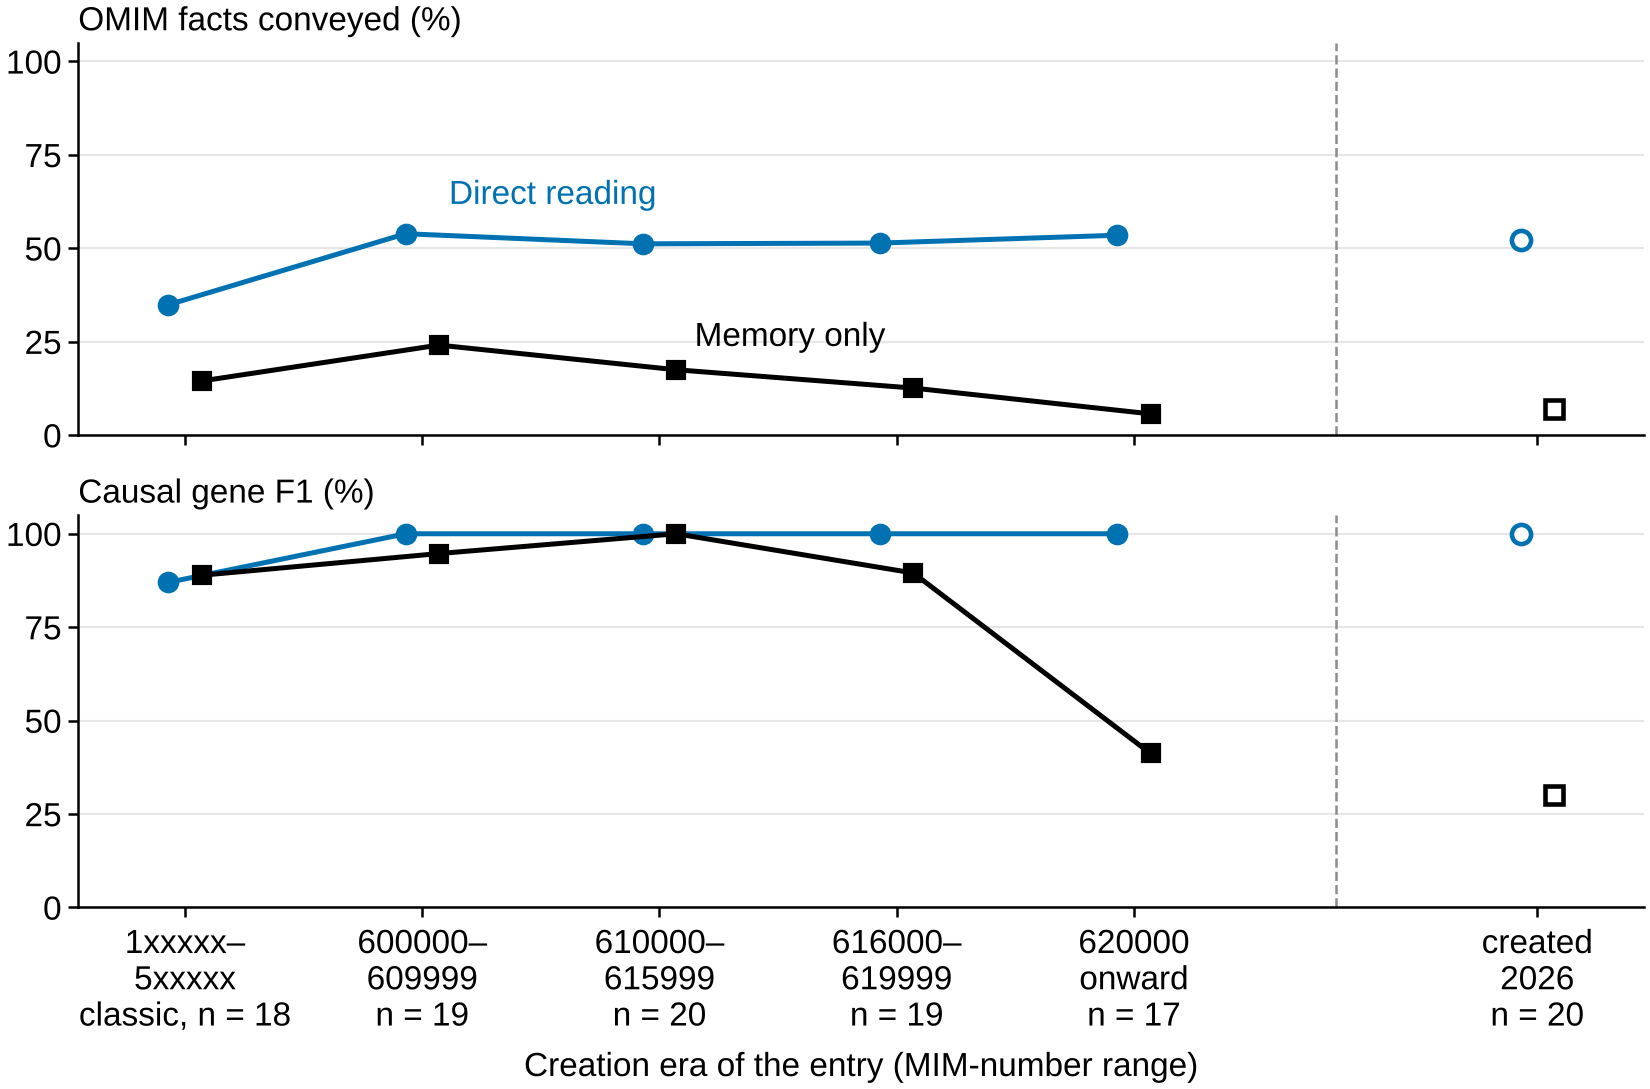
\includegraphics[width=\linewidth]{figures/fig_memory_by_era.png}
\end{center}
\caption{OMIM facts conveyed (top) and causal-gene F1 (bottom) for the memory-only control (squares) and direct reading (circles), means over the compared entries of each creation-era band (MIM-number range; $n$ per band). Hollow markers: entries created in 2026, chosen by creation date alone and not used in developing the strategies; 20 of the 30 run are compared, as stopped replies were frequent there. The model's training cut-off is not known, so this is a contamination check, not proof that reading is free of memorisation: from the 600000 band on, direct reading's coverage of facts from abstract-only papers declines with creation era (Table~\ref{tab:app_era_access}).}
\label{fig:memory}
\end{figure}

\begin{table}[!htbp]
\caption{Where the facts direct reading did not fully convey went (97 entries, 466 paragraphs, 437 judge calls, none failed; left out: 3 entries whose writer was stopped). Each missed fact was checked once against the text available for its paper; the check is a model judgement. Bottom: by whether the draft conveyed the fact not at all (absent) or less precisely (partial). Facts contradicted by the draft (7 full text, 25 abstract, 0 title; 32 in all) are not in the columns.}
\label{tab:app_missed}
\scriptsize
\begin{tabularx}{\linewidth}{>{\raggedright\arraybackslash}p{2.0cm}>{\centering\arraybackslash}X>{\centering\arraybackslash}X>{\centering\arraybackslash}X>{\centering\arraybackslash}X>{\centering\arraybackslash}X>{\centering\arraybackslash}X>{\centering\arraybackslash}X>{\centering\arraybackslash}X}
\toprule
Paper read as & OMIM facts & Conveyed & Not fully conveyed & \ldots{} in text & \ldots{} partly in text & \ldots{} not in text & Unjudged & In text, share of missed \\
\midrule
Full text & 1,837 & 1,329 & 501 & 245 & 134 & 122 & 0 & 49\% \\
Abstract only & 4,282 & 1,420 & 2,837 & 46 & 632 & 2,159 & 0 & 2\% \\
Title only & 379 & 38 & 341 & 0 & 53 & 288 & 0 & 0\% \\
All papers & 6,498 & 2,787 & 3,679 & 291 & 819 & 2,569 & 0 & 8\% \\
\bottomrule
\end{tabularx}
\vspace{4pt}
\begin{tabularx}{\linewidth}{>{\raggedright\arraybackslash}p{2.0cm}>{\centering\arraybackslash}X>{\centering\arraybackslash}X>{\centering\arraybackslash}X>{\centering\arraybackslash}X>{\centering\arraybackslash}X}
\toprule
Paper read as & Draft & Missed & \ldots{} in text & \ldots{} partly & \ldots{} not in text \\
\midrule
Full text & absent & 287 & 123 & 47 & 117 \\
Full text & partial & 214 & 122 & 87 & 5 \\
Abstract only & absent & 2,254 & 19 & 158 & 2,077 \\
Abstract only & partial & 583 & 27 & 474 & 82 \\
Title only & absent & 284 & 0 & 5 & 279 \\
Title only & partial & 57 & 0 & 48 & 9 \\
All papers & absent & 2,825 & 142 & 210 & 2,473 \\
All papers & partial & 854 & 149 & 609 & 96 \\
\bottomrule
\end{tabularx}
\end{table}

\begin{figure}[!htbp]
\begin{center}
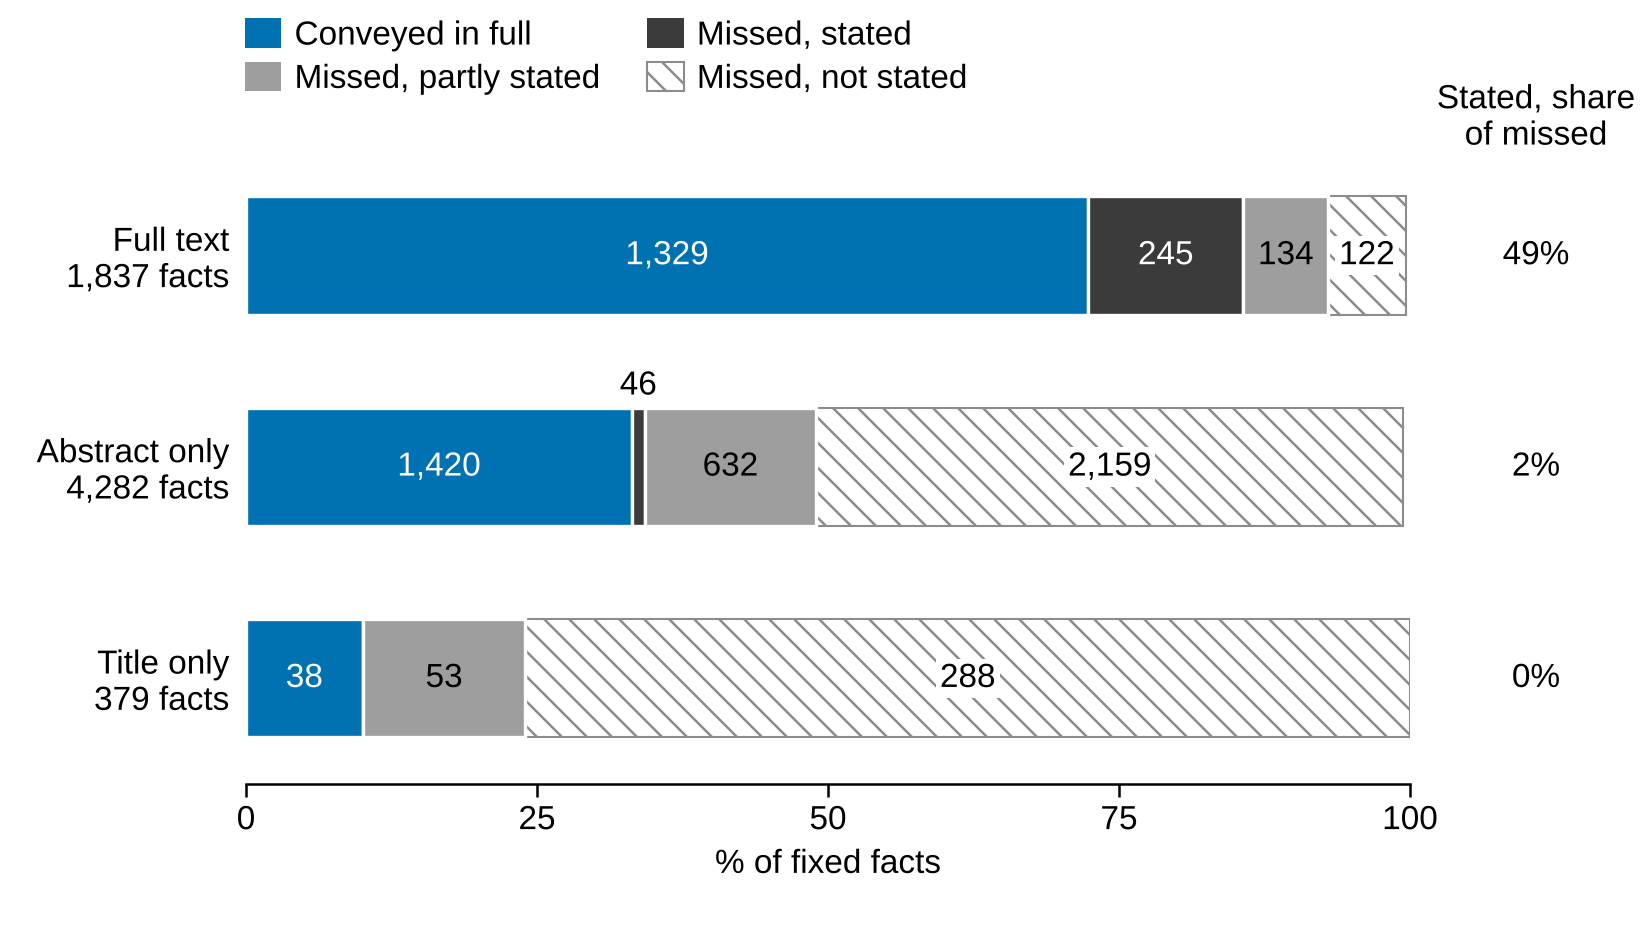
\includegraphics[width=\linewidth]{figures/fig_missed_facts.png}
\end{center}
\caption{Where the fixed facts that direct reading did not fully convey went, by how the paper could be read (pooled over facts; 97 entries with a draft, 466 paragraphs; bars labelled with fact counts). Each missed fact was checked once against the text available for its paper: stated (with a quote verified in that text), partly stated or not stated, a model judgement, not a curator's. Facts conveyed only partly count as missed; the small remainder of the full-text and abstract-only bars (7 and 25 facts) was contradicted by the draft. Right: share of missed facts the available text states.}
\label{fig:missed}
\end{figure}

\begin{table}[!htbp]
\caption{Where the facts direct reading conveyed came from (post hoc; 97 entries, 466 paragraphs; pooled over facts; left out: 3 entries whose writer was stopped). Each fact the draft conveyed in full or in part was checked against the text the writer had for the paragraph's paper(s); a fact not stated there, or stated only partly, was checked once more against the text of the entry's other supplied papers, since a later paper may describe an earlier one. No fact went unjudged. A fact stated in no supplied text may have been recalled from memory, inferred from what the text states (for example an inheritance mode from zygosity), or misjudged; these are model judgements. Shares are of the facts in the row; ``either'': conveyed in full or in part. Bottom: the second check, for facts conveyed in full or in part whose own paper's text only partly states or does not state them, against the entry's other supplied papers.}
\label{tab:app_conveyed}
\scriptsize
{\setlength{\tabcolsep}{2pt}\begin{tabularx}{\linewidth}{>{\raggedright\arraybackslash}p{1.5cm}>{\raggedright\arraybackslash}p{0.8cm}>{\centering\arraybackslash}p{0.8cm}>{\centering\arraybackslash}X>{\centering\arraybackslash}X>{\centering\arraybackslash}X>{\centering\arraybackslash}X>{\centering\arraybackslash}X}
\toprule
Paper read as & Con\-veyed & Facts & Stated in its paper's text & Partly stated in its paper's text & Stated only in another supplied paper & Partly stated only in another supplied paper & In no supplied text \\
\midrule
Full text & in full & 1,329 & 1,174 (88.3\%) & 122 (9.2\%) & 22 (1.7\%) & 4 (0.3\%) & 7 (0.5\%) \\
Full text & in part & 214 & 122 (57.0\%) & 86 (40.2\%) & 1 (0.5\%) & 1 (0.5\%) & 4 (1.9\%) \\
Full text & either & 1,543 & 1,296 (84.0\%) & 208 (13.5\%) & 23 (1.5\%) & 5 (0.3\%) & 11 (0.7\%) \\
Abstract only & in full & 1,420 & 1,061 (74.7\%) & 222 (15.6\%) & 102 (7.2\%) & 11 (0.8\%) & 24 (1.7\%) \\
Abstract only & in part & 583 & 27 (4.6\%) & 462 (79.2\%) & 15 (2.6\%) & 21 (3.6\%) & 58 (10.0\%) \\
Abstract only & either & 2,003 & 1,088 (54.3\%) & 684 (34.2\%) & 117 (5.8\%) & 32 (1.6\%) & 82 (4.1\%) \\
Title only & in full & 38 & 27 (71.0\%) & 8 (21.1\%) & 3 (7.9\%) & 0 (0.0\%) & 0 (0.0\%) \\
Title only & in part & 57 & 0 (0.0\%) & 47 (82.5\%) & 1 (1.8\%) & 1 (1.8\%) & 8 (14.0\%) \\
Title only & either & 95 & 27 (28.4\%) & 55 (57.9\%) & 4 (4.2\%) & 1 (1.1\%) & 8 (8.4\%) \\
All papers & in full & 2,787 & 2,262 (81.2\%) & 352 (12.6\%) & 127 (4.6\%) & 15 (0.5\%) & 31 (1.1\%) \\
All papers & in part & 854 & 149 (17.4\%) & 595 (69.7\%) & 17 (2.0\%) & 23 (2.7\%) & 70 (8.2\%) \\
All papers & either & 3,641 & 2,411 (66.2\%) & 947 (26.0\%) & 144 (4.0\%) & 38 (1.0\%) & 101 (2.8\%) \\
\bottomrule
\end{tabularx}}
\vspace{4pt}
{\setlength{\tabcolsep}{3pt}\begin{tabularx}{\linewidth}{>{\raggedright\arraybackslash}p{1.6cm}>{\raggedright\arraybackslash}p{1.6cm}>{\centering\arraybackslash}p{0.8cm}>{\centering\arraybackslash}X>{\centering\arraybackslash}X>{\centering\arraybackslash}X>{\centering\arraybackslash}X}
\toprule
Paper read as & Own text & Facts & Another supplied paper states it & \ldots{} partly & \ldots{} does not & No other paper supplied \\
\midrule
Full text & partly states & 223 & 15 & 37 & 171 & 0 \\
Full text & does not state & 24 & 8 & 5 & 11 & 0 \\
Abstract only & partly states & 728 & 44 & 119 & 546 & 19 \\
Abstract only & does not state & 187 & 73 & 32 & 81 & 1 \\
Title only & partly states & 57 & 2 & 5 & 50 & 0 \\
Title only & does not state & 11 & 2 & 1 & 8 & 0 \\
All papers & partly states & 1,008 & 61 & 161 & 767 & 19 \\
All papers & does not state & 222 & 83 & 38 & 100 & 1 \\
\bottomrule
\end{tabularx}}
\end{table}

\begin{table}[!htbp]
\caption{OMIM facts conveyed restricted by whether the supplied text states the fact (93 compared entries; post hoc: these restrictions, including the one to facts stated in full-text papers, were added after the first results). Each fixed fact carries one judgement of whether the text available for its paper states it, partly states it or does not state it (a model judgement; a ``stated'' verdict needs a quote verified in the text; not checked by a curator); it is the same for every strategy. Top: the facts by how the paragraph's paper could be read (pooled; identical for every strategy). Middle: coverage as mean over entries / pooled over facts; $n$ = entries with facts in the restriction. Bottom: paired differences from direct reading in points (means over entries), bootstrap 95\% interval, entries better/worse/tied. The unrestricted means reproduce Table~\ref{tab:main}; the intervals here come from a separate bootstrap and can differ from it by 0.1.}
\label{tab:app_stated}
\scriptsize
\begin{tabularx}{\linewidth}{>{\raggedright\arraybackslash}p{2.6cm}>{\centering\arraybackslash}X>{\centering\arraybackslash}X>{\centering\arraybackslash}X>{\centering\arraybackslash}X}
\toprule
Paper read as & Facts & Stated & Partly stated & Not stated \\
\midrule
Full text & 1,639 & 1,246 & 253 & 140 \\
Abstract only & 4,221 & 1,099 & 883 & 2,239 \\
Title only & 379 & 27 & 62 & 290 \\
All papers & 6,239 & 2,372 & 1,198 & 2,669 \\
\bottomrule
\end{tabularx}
\vspace{4pt}

\begin{tabularx}{\linewidth}{>{\raggedright\arraybackslash}p{2.6cm}>{\centering\arraybackslash}X>{\centering\arraybackslash}X>{\centering\arraybackslash}X>{\centering\arraybackslash}X>{\centering\arraybackslash}X>{\centering\arraybackslash}X}
\toprule
Strategy & All facts & Stated & Stated or partly & Not stated & Stated, full-text papers & Stated, abstract-only papers \\
\midrule
Direct reading & 49.1 / 48.6 & 94.4 / 91.8 & 77.5 / 80.2 & 6.9 / 6.3 & 88.5 / 87.0 & 97.1 / 97.0 \\
Agentic curator & 48.4 / 47.9 & 93.6 / 91.3 & 76.9 / 79.6 & 6.3 / 5.6 & 88.3 / 86.5 & 96.3 / 96.6 \\
Evidence graph & 48.6 / 47.6 & 94.2 / 92.9 & 77.5 / 80.5 & 5.5 / 3.5 & 90.2 / 89.0 & 96.6 / 97.2 \\
Case table first & 47.2 / 46.1 & 91.0 / 87.5 & 75.4 / 76.9 & 5.9 / 4.8 & 80.1 / 80.5 & 95.5 / 95.1 \\
Recall, then verify & 14.6 / 12.5 & 28.8 / 20.3 & 26.0 / 20.8 & 2.1 / 1.4 & 13.6 / 13.0 & 36.5 / 28.3 \\
Memory only (control) & 15.1 / 12.7 & 23.3 / 15.5 & 23.3 / 17.5 & 8.2 / 6.3 & 10.9 / 10.4 & 28.2 / 20.9 \\
Entries ($n$) / facts & 93 / 6,239 & 89 / 2,372 & 93 / 3,570 & 90 / 2,669 & 40 / 1,246 & 79 / 1,099 \\
\bottomrule
\end{tabularx}
\vspace{4pt}

{\setlength{\tabcolsep}{3pt}%
\begin{tabularx}{\linewidth}{>{\raggedright\arraybackslash}p{2.0cm}>{\centering\arraybackslash}X>{\centering\arraybackslash}X>{\centering\arraybackslash}X>{\centering\arraybackslash}X>{\centering\arraybackslash}X>{\centering\arraybackslash}X}
\toprule
Difference from direct reading & All facts & Stated & Stated or partly & Not stated & Stated, full-text papers & Stated, abstract-only papers \\
\midrule
Agentic curator & $-$0.6 ($-$1.3 to +0.0); 31/42/20 & $-$0.8 ($-$2.6 to +0.4); 20/23/46 & $-$0.7 ($-$2.0 to +0.4); 36/37/20 & $-$0.5 ($-$1.8 to +1.0); 16/27/47 & $-$0.2 ($-$1.8 to +1.2); 13/15/12 & $-$0.8 ($-$2.6 to +0.5); 11/9/59 \\
Evidence graph & $-$0.5 ($-$1.5 to +0.5); 33/45/15 & $-$0.3 ($-$2.1 to +1.3); 25/21/43 & $-$0.0 ($-$1.5 to +1.4); 41/41/11 & $-$1.4 ($-$3.4 to +0.7); 16/28/46 & +1.7 ($-$0.7 to +4.0); 18/15/7 & $-$0.5 ($-$2.5 to +1.2); 10/11/58 \\
Case table first & $-$1.9 ($-$3.1 to $-$0.7); 31/48/14 & $-$3.4 ($-$5.6 to $-$1.6); 16/42/31 & $-$2.1 ($-$3.6 to $-$0.6); 27/48/18 & $-$1.0 ($-$3.1 to +1.2); 27/26/37 & $-$8.4 ($-$14.3 to $-$3.8); 9/28/3 & $-$1.6 ($-$3.6 to +0.2); 12/21/46 \\
Recall, then verify & $-$34.5 ($-$39.3 to $-$30.0); 2/89/2 & $-$65.6 ($-$70.6 to $-$60.2); 0/84/5 & $-$51.5 ($-$55.9 to $-$47.1); 1/88/4 & $-$4.8 ($-$6.7 to $-$3.0); 11/50/29 & $-$74.9 ($-$80.2 to $-$69.3); 0/40/0 & $-$60.6 ($-$67.3 to $-$53.5); 0/71/8 \\
Memory only (control) & $-$34.0 ($-$39.2 to $-$28.7); 7/85/1 & $-$71.1 ($-$75.9 to $-$66.0); 0/85/4 & $-$54.2 ($-$59.2 to $-$48.9); 4/88/1 & +1.3 ($-$1.4 to +4.6); 37/30/23 & $-$77.6 ($-$82.5 to $-$72.3); 0/40/0 & $-$68.9 ($-$75.1 to $-$62.3); 0/74/5 \\
\bottomrule
\end{tabularx}}
\end{table}

\FloatBarrier
\section{Measurement stability}
\label{app:stability}
Judge variation: the same drafts and fact lists judged three times (top). Evidence graph minus direct reading in the three judgings: $+0.7$/$+0.5$/$+1.3$ points; per-fact agreement between two judgings of the same draft: 3,498 of 3,654 statuses (95.7\%). Run-to-run variation: generation, audit and scoring repeated three times on 30 entries (bottom). Evidence graph minus direct reading in replicates 1/2/3: $+0.7$/$+1.9$/$+0.5$ points; within-entry SD of that paired difference 5.0 points, giving a replicate-noise 95\% half-width of 1.0 point over 93 entries and 1.8 points over 30. One replicate is one sample; the main comparison is a single run per entry. The half-width is a yardstick for how much a difference of this kind moves when generation, audit and scoring are repeated; the bootstrap interval over entries is the test of a difference. On these 30 entries the evidence graph is ahead of direct reading in all three replicates and all three judgings, whereas on the 93 entries of the main comparison its difference is $-0.5$ ($-1.5$ to $+0.5$). Replicate 1 reproduces the main run on these entries, so the difference in sign comes from which entries are averaged, not from replicate noise; the replicates themselves range from $+0.5$ to $+1.9$. Crediting a fact anywhere in the draft rather than only in text citing its paper (same 30 entries): direct reading 46\% against 47\%, evidence graph 46\% against 46\%, case table first 45\% against 45\%, so strategies that pool across papers do not lose credit under another citation.

\begin{table}[!htbp]
\caption{Judge variation (top) and run-to-run variation (bottom) in OMIM facts conveyed on 30 entries.}
\label{tab:app_stability}
\scriptsize
\begin{tabularx}{\linewidth}{>{\raggedright\arraybackslash}p{2.4cm}>{\centering\arraybackslash}X>{\centering\arraybackslash}X>{\centering\arraybackslash}X}
\toprule
Strategy & Entries & Mean OMIM facts conveyed in three judgings (\%) & Mean within-entry SD across judgings (points) \\
\midrule
Direct reading & 30 & 45.6 / 45.7 / 45.3 & 0.9 \\
Evidence graph & 30 & 46.3 / 46.2 / 46.6 & 0.8 \\
\bottomrule
\end{tabularx}
\vspace{4pt}
\begin{tabularx}{\linewidth}{>{\raggedright\arraybackslash}p{2.4cm}>{\centering\arraybackslash}X>{\centering\arraybackslash}X>{\centering\arraybackslash}X>{\centering\arraybackslash}X}
\toprule
Strategy & 30-entry mean in replicates 1 / 2 / 3 (\%) & Within-entry SD (points) & Between-entry SD (points) & Share of variance within entries \\
\midrule
Direct reading & 45.6 / 44.7 / 45.9 & 2.5 & 21.0 & 1\% \\
Evidence graph & 46.3 / 46.6 / 46.4 & 4.0 & 22.1 & 3\% \\
\bottomrule
\end{tabularx}
\end{table}

\FloatBarrier
\section{Ablation of the extract-then-write strategies}
\label{app:ablation}
The 40-entry subset contains every entry with at least half its papers readable in full that all reading strategies completed, filled to 40 with entries drawn at random to bring each creation-era band to 8 entries; 22 of the 40 have at least half their papers readable in full and 29 have at least one, so absolute levels are higher than in the main comparison. 38 were completed by all seven strategies. The two changes in \emph{matched} (high-effort extraction; writer-chosen synopsis terms and, for the table, inheritance) were made together; since choosing synopsis terms cannot change which facts or variants are extracted, attributing the change in facts, claims and variants to extraction effort is an inference. Also giving the writer the papers' text (\emph{plus text}) raises claims judged supported, not facts (Table~\ref{tab:app_abl_diff}).

\textbf{The ablation set and the main comparison.} The ablation reuses the main run's drafts for direct reading, the evidence graph and case table first: on all 38 entries the drafts and fact marks are identical, so these rows give the main settings on the ablation's entries, and they differ from the main comparison's estimates only in which entries are averaged. By the main comparison's access groups the 38 entries comprise 11 with no full text, 7 with under half, 19 with half or more and 1 with all papers in full text; all are among the main comparison's 93 entries. At the main settings, the evidence graph is $+1.0$ against direct reading on these 38 entries and case table first $-2.3$ (Table~\ref{tab:app_abl_main}), against $-0.5$ and $-1.9$ on all 93 (Table~\ref{tab:main}). Of the main comparison's 21 entries with half or more full text (Table~\ref{tab:app_strata}), 19 are in the ablation set (the other two are among the entries a matched or plus-text variant did not complete); on those 19 the evidence graph is at $-1.2$ ($-3.8$ to $+1.3$; better/worse/tied 7/10/2) and case table first at $-6.2$ ($-8.6$ to $-3.5$; 3/16/0). On the ablation's other 19 entries (no full text, under half, or all full text): evidence graph $+3.1$ ($+1.0$ to $+5.6$; 12/5/2), case table first $+1.5$ ($-1.1$ to $+4.7$; 10/8/1). The matched evidence graph's $+1.8$ against direct reading is therefore mostly the $+1.0$ these entries already show at the main settings, with a settings step of $+0.8$ whose interval includes zero; the clear settings effect is the case table's step of $+2.1$.

Completion: direct reading, the evidence graph and case table first completed all 40; the matched and plus-text graph variants each lost one entry and the matched and plus-text table variants two, because the safety filter stopped a high-effort extraction call for a paper that had gone through at medium effort. Generation cost per entry at list price: direct reading \$0.32, evidence graph \$0.65, matched \$0.72, plus text \$0.88, case table first \$0.72, matched \$0.84, plus text \$0.97; with audit and scoring: \$1.59, \$2.00, \$2.14, \$2.25, \$2.07, \$2.26, \$2.29. Variant precision (share of a draft's variants that are OMIM's) in this ablation: direct reading 87.8\%, evidence graph 81.4\%, graph plus text 84.4\%, case table first matched 76.5\%, case table first plus text 85.0\%.

\begin{table}[!htbp]
\caption{Matched ablation beside the main settings on the same 38 entries (post hoc; means over entries). The main-settings rows reuse the main run's drafts and fact marks. Facts: OMIM facts conveyed (\%). $\Delta$: difference from direct reading; Step: matched minus main settings for the same strategy; both in points with bootstrap 95\% interval over entries and entries better/worse. Supp.: claims judged supported (\%); HPO F1: synopsis exact F1 (\%); Var.\ rec.\ and prec.: OMIM variants recovered and variant precision (\%). Price: generation list price per entry. ---: not applicable (the baseline, or no step at the main settings). n/r: not reported for this arm by the ablation's comparison.}
\label{tab:app_abl_main}
\scriptsize
\setlength{\tabcolsep}{2pt}
\begin{tabularx}{\linewidth}{>{\raggedright\arraybackslash}p{2.6cm}>{\centering\arraybackslash}p{0.55cm}>{\centering\arraybackslash}X>{\centering\arraybackslash}X>{\centering\arraybackslash}p{0.55cm}>{\centering\arraybackslash}p{0.6cm}>{\centering\arraybackslash}p{0.6cm}>{\centering\arraybackslash}p{0.6cm}>{\centering\arraybackslash}p{0.65cm}}
\toprule
Strategy, settings & Facts & $\Delta$ facts (95\% CI); b/w & Step (95\% CI); b/w & Supp. & HPO F1 & Var.\ rec. & Var.\ prec. & Price \\
\midrule
Direct reading & 58.4 & --- & --- & 97.9 & 40.1 & 77.3 & 87.8 & \$0.32 \\
Evidence graph, main & 59.4 & +1.0 ($-$0.9 to +2.8); 19/15 & --- & 97.1 & 37.6 & 76.8 & 81.4 & \$0.65 \\
Evidence graph, matched & 60.2 & +1.8 (+0.4 to +3.3); 24/10 & +0.8 ($-$0.5 to +2.1); 18/12 & 96.8 & 37.8 & 77.0 & n/r & \$0.72 \\
Case table, main & 56.1 & $-$2.3 ($-$4.5 to +0.1); 13/24 & --- & 96.0 & 37.3 & 74.4 & n/r & \$0.72 \\
Case table, matched & 58.3 & $-$0.2 ($-$2.4 to +2.1); 16/20 & +2.1 (+1.1 to +3.2); 25/8 & 97.0 & 38.3 & 73.7 & 76.5 & \$0.84 \\
\bottomrule
\end{tabularx}
\end{table}

\begin{table}[!htbp]
\caption{Ablation: means over the 38 entries completed by all seven strategies.}
\label{tab:app_abl_means}
\scriptsize
\begin{tabularx}{\linewidth}{>{\raggedright\arraybackslash}p{3.0cm}>{\centering\arraybackslash}X>{\centering\arraybackslash}X>{\centering\arraybackslash}X>{\centering\arraybackslash}X>{\centering\arraybackslash}X>{\centering\arraybackslash}X>{\centering\arraybackslash}X}
\toprule
Measure & Direct reading & Evidence graph & Evidence graph, matched & Evidence graph plus text & Case table first & Case table first, matched & Case table first plus text \\
\midrule
OMIM facts conveyed (\%) & 58.4 & 59.4 & 60.2 & 60.2 & 56.1 & 58.3 & 59.1 \\
\ldots{} on papers readable in full (\%) & 80.4 (n=25) & 82.7 (n=25) & 83.7 (n=25) & 83.0 (n=25) & 75.4 (n=25) & 78.8 (n=25) & 79.9 (n=25) \\
Claims judged supported (\%) & 97.9 & 97.1 & 96.8 & 98.3 & 96.0 & 97.0 & 98.1 \\
Synopsis precision (\%) & 45.2 & 40.5 & 39.4 & 42.6 & 40.6 & 41.2 & 42.0 \\
Synopsis recall (\%) & 43.8 & 44.5 & 44.9 & 44.1 & 46.3 & 44.1 & 44.4 \\
Synopsis exact F1 (\%) & 40.1 & 37.6 & 37.8 & 39.5 & 37.3 & 38.3 & 39.4 \\
Synopsis terms per entry & 19.0 & 25.2 & 24.0 & 21.2 & 29.9 & 22.5 & 20.3 \\
Inheritance matches (\%) & 97.4 & 94.7 & 94.7 & 94.7 & 94.7 & 97.4 & 97.4 \\
Variants recovered (\%) & 77.3 & 76.8 & 77.0 & 77.4 & 74.4 & 73.7 & 72.7 \\
\bottomrule
\end{tabularx}
\end{table}

\begin{table}[!htbp]
\caption{Ablation: each step against the one before it (top) and each strategy against direct reading (bottom); difference, 95\% bootstrap interval, entries better/worse. Points except synopsis terms.}
\label{tab:app_abl_diff}
\scriptsize
\setlength{\tabcolsep}{3pt}
\begin{tabularx}{\linewidth}{>{\raggedright\arraybackslash}p{2.2cm}>{\centering\arraybackslash}X>{\centering\arraybackslash}X>{\centering\arraybackslash}X>{\centering\arraybackslash}X}
\toprule
Measure & Graph matched $-$ graph & Graph plus text $-$ graph matched & Table matched $-$ table & Table plus text $-$ table matched \\
\midrule
OMIM facts conveyed & +0.8 ($-$0.5 to +2.1); 18/12 & +0.0 ($-$0.8 to +0.9); 16/16 & +2.1 (+1.1 to +3.2); 25/8 & +0.8 ($-$0.8 to +2.6); 21/13 \\
\ldots{} on papers readable in full & +1.0 ($-$1.0 to +3.0); 13/8 & $-$0.7 ($-$1.9 to +0.6); 8/15 & +3.3 (+1.6 to +5.1); 17/4 & +1.1 ($-$1.6 to +3.8); 13/9 \\
Claims judged supported & $-$0.3 ($-$0.9 to +0.4); 15/22 & +1.5 (+0.9 to +2.1); 31/6 & +0.9 ($-$0.3 to +2.4); 22/15 & +1.2 (+0.3 to +2.2); 23/12 \\
Synopsis precision & $-$1.1 ($-$3.7 to +1.5); 12/19 & +3.2 (+1.2 to +5.4); 21/7 & +0.6 ($-$3.9 to +4.8); 17/11 & +0.8 ($-$1.9 to +3.2); 17/10 \\
Synopsis recall & +0.4 ($-$2.8 to +3.6); 10/14 & $-$0.8 ($-$3.2 to +1.6); 6/10 & $-$2.3 ($-$5.6 to +0.8); 9/10 & +0.3 ($-$2.1 to +3.2); 7/10 \\
Synopsis exact F1 & +0.2 ($-$2.2 to +2.8); 15/18 & +1.7 ($-$0.1 to +3.6); 17/11 & +1.0 ($-$2.0 to +3.5); 18/11 & +1.1 ($-$0.8 to +3.1); 15/12 \\
Synopsis terms per entry & $-$1.2 ($-$3.6 to +0.8); 16/14 & $-$2.8 ($-$5.4 to $-$0.5); 9/20 & $-$7.4 ($-$13.7 to $-$2.2); 10/18 & $-$2.2 ($-$3.7 to $-$0.7); 8/17 \\
Inheritance matches & +0.0 (+0.0 to +0.0); 0/0 & +0.0 (+0.0 to +0.0); 0/0 & +2.6 (+0.0 to +7.9); 1/0 & +0.0 (+0.0 to +0.0); 0/0 \\
Variants recovered & +0.2 (+0.0 to +0.7); 1/0 & +0.4 (+0.0 to +1.1); 1/0 & $-$0.7 ($-$3.9 to +2.0); 1/1 & $-$1.0 ($-$6.3 to +3.6); 4/3 \\
\bottomrule
\end{tabularx}
\vspace{4pt}
\begin{tabularx}{\linewidth}{>{\raggedright\arraybackslash}p{2.2cm}>{\centering\arraybackslash}X>{\centering\arraybackslash}X>{\centering\arraybackslash}X>{\centering\arraybackslash}X>{\centering\arraybackslash}X>{\centering\arraybackslash}X}
\toprule
Measure & Evidence graph & Graph matched & Graph plus text & Case table first & Table matched & Table plus text \\
\midrule
OMIM facts conveyed & +1.0 ($-$0.9 to +2.8); 19/15 & +1.8 (+0.4 to +3.3); 24/10 & +1.8 (+0.5 to +3.2); 24/10 & $-$2.3 ($-$4.5 to +0.1); 13/24 & $-$0.2 ($-$2.4 to +2.1); 16/20 & +0.6 ($-$1.1 to +2.6); 18/15 \\
\ldots{} on papers readable in full & +2.3 ($-$0.2 to +5.0); 13/11 & +3.3 (+1.2 to +5.6); 17/6 & +2.7 (+0.5 to +5.0); 16/5 & $-$4.9 ($-$8.0 to $-$1.4); 6/19 & $-$1.6 ($-$4.8 to +1.9); 7/16 & $-$0.5 ($-$3.7 to +2.8); 11/9 \\
Claims judged supported & $-$0.8 ($-$1.4 to $-$0.1); 8/25 & $-$1.0 ($-$1.8 to $-$0.2); 12/24 & +0.4 ($-$0.3 to +1.2); 20/11 & $-$1.8 ($-$3.3 to $-$0.6); 11/25 & $-$0.9 ($-$2.1 to +0.2); 14/22 & +0.3 ($-$0.4 to +1.1); 21/14 \\
Synopsis precision & $-$4.6 ($-$8.3 to $-$1.1); 9/24 & $-$5.7 ($-$9.2 to $-$2.1); 7/29 & $-$2.6 ($-$5.5 to +0.4); 12/22 & $-$4.5 ($-$8.5 to $-$0.5); 9/26 & $-$3.9 ($-$8.1 to $-$0.1); 13/24 & $-$3.1 ($-$7.2 to +0.3); 14/19 \\
Synopsis recall & +0.8 ($-$3.9 to +5.0); 15/8 & +1.1 ($-$2.3 to +4.5); 15/10 & +0.3 ($-$3.0 to +3.1); 12/9 & +2.6 ($-$2.4 to +7.7); 17/12 & +0.3 ($-$3.9 to +4.4); 15/11 & +0.6 ($-$2.0 to +3.3); 11/9 \\
Synopsis exact F1 & $-$2.5 ($-$5.1 to +0.1); 10/24 & $-$2.3 ($-$4.5 to $-$0.1); 11/24 & $-$0.6 ($-$2.6 to +1.2); 14/20 & $-$2.8 ($-$5.6 to +0.2); 15/21 & $-$1.8 ($-$4.8 to +1.0); 16/21 & $-$0.7 ($-$3.2 to +1.6); 17/16 \\
Synopsis terms per entry & +6.2 (+3.1 to +9.8); 25/7 & +5.0 (+2.3 to +8.1); 27/8 & +2.2 (+0.7 to +3.8); 21/12 & +10.8 (+4.6 to +18.1); 22/10 & +3.5 (+1.5 to +5.8); 24/10 & +1.3 ($-$0.0 to +2.6); 19/11 \\
Inheritance matches & $-$2.6 ($-$7.9 to +0.0); 0/1 & $-$2.6 ($-$7.9 to +0.0); 0/1 & $-$2.6 ($-$7.9 to +0.0); 0/1 & $-$2.6 ($-$7.9 to +0.0); 0/1 & +0.0 (+0.0 to +0.0); 0/0 & +0.0 (+0.0 to +0.0); 0/0 \\
Variants recovered & $-$0.6 ($-$1.5 to +0.0); 0/2 & $-$0.3 ($-$1.0 to +0.0); 0/1 & +0.0 ($-$1.0 to +1.1); 1/1 & $-$3.0 ($-$7.2 to $-$0.2); 0/4 & $-$3.6 ($-$8.2 to $-$0.2); 0/4 & $-$4.7 ($-$10.9 to $-$0.3); 1/4 \\
\bottomrule
\end{tabularx}
\end{table}

\FloatBarrier
\section{Hidden-full-text experiment and second-hand evidence}
\label{app:hidden}
Open-access papers that cite and describe each target paper were searched for all 515 papers through Europe PMC; passages (paragraphs or table rows whose citation points at the target paper) were found for 473 papers (326 of 345 abstract-only, 53 of 74 title-only, 94 of 96 full-text): 2,430 passages. The hidden-full-text experiment used the 49 entries with a full-text paper that an in-scope curator paragraph is about and hid all 91 of their full-text papers (81 of the 96 full-text papers have an in-scope paragraph); the other 5 full-text papers, in 5 entries, have no in-scope paragraph, so hiding them could not change the score. All 91 hidden papers have citing papers, 89 have open-access citing papers and at least one passage, and they received 523 passages. Over all 49 entries the two new conditions convey 35.3\% (abstract only) and 41.1\% (abstract plus second-hand) under the earlier scoring, pooled over facts. Under the earlier scoring facts are split separately for each condition, so the fact counts differ slightly.

\begin{table}[!htbp]
\caption{Hidden-full-text experiment, 46 entries and 136 paragraphs in every condition. The facts are those of every in-scope paragraph about a hidden paper (2,120). The by-access tables (Tables~\ref{tab:app_access}, \ref{tab:app_stated}) class a paragraph about several papers by its least readable paper: on that rule 1,837 of these facts, in 44 entries, are classed as full text and 283 as abstract or title only, and those tables are further restricted to the 93 entries every strategy completed. Top: fixed fact lists (main measure), coverage pooled over facts and as a mean over entries, with the earlier per-draft scoring (pooled) beside it. The full-text draft is the main run's direct-reading draft; it went through the repair round and was also scored before repair (a post hoc rescoring, so that no arm is repaired); the two abstract drafts were not repaired. Before repair the audit flagged 13 of 6,609 audited claims (13 unsupported, 0 contradicted) in 11 paragraphs of 8 entries; repair revised those 11 paragraphs and deleted none. The draft before repair was reconstructed from the stored writer and audit replies without new generation (taking it through the repair round reproduces the final draft exactly). Middle: paired differences, means over entries. Bottom: earlier scoring, pooled over facts. ---: not computed (the draft before repair was scored only on the fixed fact lists).}
\label{tab:app_hidden}
\scriptsize
{\setlength{\tabcolsep}{2pt}\begin{tabularx}{\linewidth}{>{\raggedright\arraybackslash}p{2.2cm}>{\centering\arraybackslash}X>{\centering\arraybackslash}X>{\centering\arraybackslash}X>{\centering\arraybackslash}X>{\centering\arraybackslash}X>{\centering\arraybackslash}X>{\centering\arraybackslash}X>{\centering\arraybackslash}X>{\centering\arraybackslash}X>{\centering\arraybackslash}X}
\toprule
Condition & Entries & Para\-graphs & Facts judged & Present & Partial & Absent & Contra\-dicted & Coverage, pooled over facts & Coverage, mean over entries & Earlier scoring, pooled \\
\midrule
Abstract only & 46 & 136 & 2,120 & 495 & 331 & 1,290 & 4 & 31.2\% & 36.1\% & 35.5\% \\
Abstract + second-hand & 46 & 136 & 2,120 & 629 & 297 & 1,184 & 10 & 36.7\% & 40.9\% & 41.4\% \\
Full text, before repair & 46 & 136 & 2,120 & 1,511 & 255 & 344 & 10 & 77.3\% & 79.8\% & --- \\
Full text, after repair & 46 & 136 & 2,120 & 1,513 & 254 & 343 & 10 & 77.4\% & 79.9\% & 78.6\% \\
\bottomrule
\end{tabularx}}
\vspace{4pt}
\begin{tabularx}{\linewidth}{>{\raggedright\arraybackslash}p{3.4cm}>{\centering\arraybackslash}X>{\centering\arraybackslash}X>{\centering\arraybackslash}X>{\centering\arraybackslash}X>{\centering\arraybackslash}X}
\toprule
Difference (mean over entries) & Entries & Fixed lists: mean (95\% CI) & better / worse / tied & Earlier scoring: mean (95\% CI) & better / worse / tied \\
\midrule
Abstract + second-hand minus abstract only & 46 & +4.9 (+2.8 to +7.1) & 33 / 9 / 4 & +5.3 (+3.6 to +7.2) & 36 / 7 / 3 \\
Full text before repair minus abstract only & 46 & +43.7 (+38.3 to +49.1) & 45 / 0 / 1 & --- & --- \\
Full text after repair minus abstract only & 46 & +43.9 (+38.5 to +49.3) & 45 / 0 / 1 & +41.7 (+36.7 to +46.6) & 46 / 0 / 0 \\
Full text after minus before repair & 46 & +0.2 ($-$0.1 to +0.4) & 6 / 2 / 38 & --- & --- \\
\bottomrule
\end{tabularx}
\vspace{4pt}
\begin{tabularx}{\linewidth}{>{\raggedright\arraybackslash}p{2.6cm}>{\centering\arraybackslash}X>{\centering\arraybackslash}X>{\centering\arraybackslash}X>{\centering\arraybackslash}X>{\centering\arraybackslash}X>{\centering\arraybackslash}X>{\centering\arraybackslash}X}
\toprule
Condition & Paragraphs & Facts & Present & Partial & Absent & Contra\-dicted & Coverage \\
\midrule
Abstract only & 136 & 1783 & 452 & 362 & 966 & 3 & 35.5\% \\
Abstract + second-hand & 136 & 1802 & 565 & 362 & 864 & 11 & 41.4\% \\
Full text, after repair & 136 & 1767 & 1268 & 243 & 246 & 10 & 78.6\% \\
\bottomrule
\end{tabularx}
\end{table}

\begin{table}[!htbp]
\caption{Claims about the hidden papers in the second-hand draft (2,308 claims; 2,208 after collapsing a statement repeated in two paragraphs), audited against what the writer saw and against the full text. \emph{own}: the auditor's quote is in the paper's title or abstract; \emph{second-hand}: in a later paper's passage; \emph{none}: no quote (judged unsupported or contradicted against what the writer saw). Middle and bottom: second-hand claims by passage kind and by the number of other references the passage cites (few = at most 2). Full texts exclude supplementary material, so ``unsupported'' is an upper bound on error; ``contradicted'' is not affected in the same way.}
\label{tab:app_secondhand_claims}
\scriptsize
\begin{tabularx}{\linewidth}{>{\raggedright\arraybackslash}p{3.4cm}>{\centering\arraybackslash}X>{\centering\arraybackslash}X>{\centering\arraybackslash}X>{\centering\arraybackslash}X>{\centering\arraybackslash}X>{\centering\arraybackslash}X}
\toprule
Evidence (audit of what the writer saw) & Claims (collapsed) & Full text: supported & partial & unsupported & contradicted & no verdict \\
\midrule
none & 340 (338) & 191 (191) & 59 (59) & 55 (55) & 8 (8) & 27 (25) \\
own & 1856 (1764) & 1688 (1598) & 136 (134) & 8 (8) & 6 (6) & 18 (18) \\
second-hand & 112 (106) & 74 (68) & 24 (24) & 11 (11) & 3 (3) & 0 (0) \\
\bottomrule
\end{tabularx}
\vspace{4pt}
\begin{tabularx}{\linewidth}{>{\raggedright\arraybackslash}p{3.4cm}>{\centering\arraybackslash}X>{\centering\arraybackslash}X>{\centering\arraybackslash}X>{\centering\arraybackslash}X>{\centering\arraybackslash}X>{\centering\arraybackslash}X}
\toprule
Passage kind & Claims (collapsed) & Full text: supported & partial & unsupported & contradicted & no verdict \\
\midrule
paragraph & 91 (86) & 68 (63) & 18 (18) & 2 (2) & 3 (3) & 0 (0) \\
table & 21 (20) & 6 (5) & 6 (6) & 9 (9) & 0 (0) & 0 (0) \\
\bottomrule
\end{tabularx}
\vspace{4pt}
\begin{tabularx}{\linewidth}{>{\raggedright\arraybackslash}p{3.4cm}>{\centering\arraybackslash}X>{\centering\arraybackslash}X>{\centering\arraybackslash}X>{\centering\arraybackslash}X>{\centering\arraybackslash}X>{\centering\arraybackslash}X}
\toprule
Other references cited by the passage (few = at most 2) & Claims (collapsed) & Full text: supported & partial & unsupported & contradicted & no verdict \\
\midrule
few & 87 (83) & 55 (51) & 20 (20) & 11 (11) & 1 (1) & 0 (0) \\
many & 25 (23) & 19 (17) & 4 (4) & 0 (0) & 2 (2) & 0 (0) \\
\bottomrule
\end{tabularx}
\end{table}

\begin{table}[!htb]
\caption{Second-hand evidence in use on the 96 entries both strategies completed: means over entries (top), paired difference from direct reading (middle), and coverage by access level pooled over facts (bottom). 361 of the 401 papers not readable in full received passages (1,808); 240 of 10,597 audited claims, in 92 paragraphs, rested only on second-hand text, were labelled as not checked against the cited paper and leave the denominator of claims judged supported. The writer did not name a later paper in any entry.}
\label{tab:app_secondhand}
\scriptsize
\begin{tabularx}{\linewidth}{>{\raggedright\arraybackslash}p{5.6cm}>{\centering\arraybackslash}X>{\centering\arraybackslash}X}
\toprule
Metric & Direct reading & Second-hand evidence \\
\midrule
Claims judged supported by cited paper $\uparrow$ & 96.2\% & 94.4\% \\
\ldots{} unsupported, before the repair round $\downarrow$ & 0.4\% & 3.9\% \\
\ldots{} contradicted, before the repair round $\downarrow$ & 0.0\% & 0.0\% \\
OMIM per-paper facts conveyed (primary endpoint) $\uparrow$ & 50.4\% & 52.2\% \\
\ldots{} fully (no partial credit) $\uparrow$ & 43.7\% & 45.9\% \\
OMIM per-paper facts contradicted $\downarrow$ & 0.4\% & 0.7\% \\
\ldots{} facts split afresh for each draft (earlier scoring) $\uparrow$ & 53.2\% & 54.0\% \\
Clinical synopsis HPO F1, exact $\uparrow$ & 35.9\% & 37.0\% \\
\ldots{} precision $\uparrow$ & 43.7\% & 43.2\% \\
\ldots{} recall $\uparrow$ & 36.2\% & 37.5\% \\
Clinical synopsis HPO F1, hierarchical $\uparrow$ & 56.7\% & 58.9\% \\
OMIM allelic variants recovered $\uparrow$ & 68.2\% & 73.2\% \\
Generated variants that are OMIM variants (precision) $\uparrow$ & 88.4\% (n=85) & 86.8\% (n=89) \\
Causal gene F1 $\uparrow$ & 97.6\% & 97.6\% \\
\ldots{} recall $\uparrow$ & 97.4\% & 97.4\% \\
Inheritance matches OMIM $\uparrow$ & 93.8\% & 95.8\% \\
OMIM references used $\uparrow$ & 94.6\% & 94.5\% \\
\bottomrule
\end{tabularx}
\vspace{4pt}
\begin{tabularx}{\linewidth}{>{\raggedright\arraybackslash}p{5.6cm}>{\centering\arraybackslash}X}
\toprule
Metric & Second-hand evidence \\
\midrule
Claims judged supported by cited paper $\uparrow$ & $-$1.8 ($-$2.9 to $-$0.8); 31/60/5 \\
\ldots{} unsupported, before the repair round $\downarrow$ & +3.6 (+2.2 to +5.1); 8/51/37 \\
OMIM per-paper facts conveyed (primary) $\uparrow$ & +1.8 (+1.0 to +2.8); 49/31/16 \\
OMIM per-paper facts contradicted $\downarrow$ & +0.2 (+0.0 to +0.5); 4/11/81 \\
Clinical synopsis HPO F1, exact $\uparrow$ & +1.1 ($-$0.7 to +3.0); 42/36/18 \\
Clinical synopsis HPO F1, hierarchical $\uparrow$ & +2.2 (+0.4 to +4.3); 50/36/10 \\
OMIM allelic variants recovered $\uparrow$ & +5.0 (+1.3 to +9.2); 13/2/81 \\
Causal gene F1 $\uparrow$ & +0.0 (+0.0 to +0.0); 0/0/96 \\
Inheritance matches OMIM $\uparrow$ & +2.1 (+0.0 to +5.2); 2/0/94 \\
\bottomrule
\end{tabularx}
\vspace{4pt}
\begin{tabularx}{\linewidth}{>{\raggedright\arraybackslash}p{5.6cm}>{\centering\arraybackslash}X>{\centering\arraybackslash}X}
\toprule
Paper readable as & Direct reading & Second-hand evidence \\
\midrule
full text & 78.2\% (1,837) & 78.0\% (1,837) \\
abstract & 40.4\% (4,205) & 41.7\% (4,205) \\
title & 17.5\% (379) & 26.7\% (379) \\
\bottomrule
\end{tabularx}
\end{table}

\FloatBarrier
\section{Reconciled case database and learned curation guide}
\label{app:addons}
\textbf{Reconciliation.} Over the 100 entries, reconciliation proposed 57 merges of patient or family records and accepted 40 (17 rejected by the verifier) in 27 entries; it merged 11 variant names and found 57 conflicts between papers. Counted individuals went from 2,580 to 2,413 (net; counts rose in a few entries where a re-report gave a larger family size) and families from 1,126 to 1,092. A planted test on six entries merged 10 of 10 copied reports with their originals and merged no unrelated records; this easy case shows only that a stated re-report is caught. The accepted merges were not checked by a person. Cost: one or two extra calls per entry. None of the entry-level measures uses patient counts, so no change in them is expected. Agreement of the table's patient-count fractions with those in the HPO annotations (about 560 terms) was 48\% before and after, with a mean absolute difference of 0.26; each reference fraction comes from one source while the table pools all papers.

\textbf{Learned guide.} Training (27 of 30 training entries had a direct-reading draft; scored without the audit, with the earlier per-draft fact splitting): baseline OMIM facts conveyed 53.8\% and synopsis exact F1 36.6\%. Round 1 changed facts by $+0.14$ points and synopsis F1 by $+1.29$; round 2 by $-1.41$ and $+3.57$. The text rules of round 1 and the synopsis rules of round 2 were selected by a rule fixed in advance. The final guide, run once more on the training entries: facts $+0.06$ points, synopsis F1 $+1.28$ points. A first guide, learned before stopped replies were recorded, had treated three empty drafts as omissions and was discarded. On the held-out entries, a draft makes about twice as many statements about a paper as the OMIM paragraph has facts (direct reading 24.0 statements per paper, with the guide 22.2, against 11.9 facts), and 24\% (direct) and 25\% (guide) of a draft's statements have a counterpart in that paragraph; the paragraph is variant-centred, so this is a lower bound on agreement with the entry.

\begin{table}[!htb]
\caption{Reconciled case database: paired difference from case table first on the 97 entries both completed (points, 95\% interval, better/worse/same).}
\label{tab:app_recon}
\scriptsize
\begin{tabularx}{\linewidth}{>{\raggedright\arraybackslash}p{5.6cm}>{\centering\arraybackslash}X}
\toprule
Metric & Reconciled case database \\
\midrule
Claims judged supported by cited paper $\uparrow$ & +0.0 ($-$0.4 to +0.4); 15/13/69 \\
\ldots{} unsupported, before the repair round $\downarrow$ & +0.1 ($-$0.0 to +0.3); 4/12/81 \\
OMIM per-paper facts conveyed (primary) $\uparrow$ & +0.1 ($-$0.1 to +0.4); 12/10/75 \\
OMIM per-paper facts contradicted $\downarrow$ & +0.1 ($-$0.0 to +0.2); 2/4/91 \\
Clinical synopsis HPO F1, exact $\uparrow$ & $-$0.1 ($-$0.4 to +0.3); 6/5/86 \\
Clinical synopsis HPO F1, hierarchical $\uparrow$ & +0.0 ($-$0.0 to +0.1); 2/1/94 \\
OMIM allelic variants recovered $\uparrow$ & +0.1 (+0.0 to +0.3); 1/0/96 \\
Causal gene F1 $\uparrow$ & +0.0 (+0.0 to +0.0); 0/0/97 \\
Inheritance matches OMIM $\uparrow$ & +0.0 (+0.0 to +0.0); 0/0/97 \\
\bottomrule
\end{tabularx}
\end{table}

\begin{table}[!htb]
\caption{Learned curation guide on the 68 held-out entries both strategies completed (of 70): means (top) and paired difference from direct reading (bottom).}
\label{tab:app_guide}
\scriptsize
\begin{tabularx}{\linewidth}{>{\raggedright\arraybackslash}p{5.6cm}>{\centering\arraybackslash}X>{\centering\arraybackslash}X}
\toprule
Metric & Direct reading & Learned curation guide \\
\midrule
Claims judged supported by cited paper $\uparrow$ & 96.2\% & 96.1\% \\
\ldots{} unsupported, before the repair round $\downarrow$ & 0.2\% & 0.2\% \\
\ldots{} contradicted, before the repair round $\downarrow$ & 0.0\% & 0.0\% \\
OMIM per-paper facts conveyed (primary endpoint) $\uparrow$ & 49.3\% & 50.3\% \\
\ldots{} fully (no partial credit) $\uparrow$ & 42.5\% & 43.9\% \\
OMIM per-paper facts contradicted $\downarrow$ & 0.4\% & 0.4\% \\
\ldots{} facts split afresh for each draft (earlier scoring) $\uparrow$ & 52.2\% & 51.9\% \\
Clinical synopsis HPO F1, exact $\uparrow$ & 35.7\% & 36.5\% \\
\ldots{} precision $\uparrow$ & 43.8\% & 43.0\% \\
\ldots{} recall $\uparrow$ & 37.1\% & 40.0\% \\
Clinical synopsis HPO F1, hierarchical $\uparrow$ & 55.4\% & 55.4\% \\
OMIM allelic variants recovered $\uparrow$ & 66.6\% & 65.0\% \\
Generated variants that are OMIM variants (precision) $\uparrow$ & 86.8\% (n=57) & 87.9\% (n=57) \\
Causal gene F1 $\uparrow$ & 98.0\% & 98.0\% \\
\ldots{} recall $\uparrow$ & 97.8\% & 97.8\% \\
Inheritance matches OMIM $\uparrow$ & 94.1\% & 94.1\% \\
OMIM references used $\uparrow$ & 94.5\% & 93.7\% \\
\bottomrule
\end{tabularx}
\vspace{4pt}
\begin{tabularx}{\linewidth}{>{\raggedright\arraybackslash}p{5.6cm}>{\centering\arraybackslash}X}
\toprule
Metric & Learned curation guide \\
\midrule
Claims judged supported by cited paper $\uparrow$ & $-$0.1 ($-$1.0 to +1.0); 29/35/4 \\
\ldots{} unsupported, before the repair round $\downarrow$ & $-$0.0 ($-$0.4 to +0.3); 6/7/55 \\
OMIM per-paper facts conveyed (primary) $\uparrow$ & +1.0 (+0.0 to +2.0); 30/25/13 \\
OMIM per-paper facts contradicted $\downarrow$ & +0.1 ($-$0.1 to +0.2); 3/3/62 \\
Clinical synopsis HPO F1, exact $\uparrow$ & +0.8 ($-$0.8 to +2.4); 34/22/12 \\
Clinical synopsis HPO F1, hierarchical $\uparrow$ & +0.1 ($-$1.3 to +1.4); 27/31/10 \\
OMIM allelic variants recovered $\uparrow$ & $-$1.6 ($-$3.7 to +0.0); 0/3/65 \\
Causal gene F1 $\uparrow$ & +0.0 (+0.0 to +0.0); 0/0/68 \\
Inheritance matches OMIM $\uparrow$ & +0.0 (+0.0 to +0.0); 0/0/68 \\
\bottomrule
\end{tabularx}
\end{table}

\FloatBarrier
\FloatBarrier
\section{Reading better: full results}
\label{app:better}
\textbf{Design.} Ten approaches were reviewed; the three judged most likely to help at feasible cost (checklist, completeness pass, three-draft merge) were implemented, piloted on three training entries with the prompts then frozen, and evaluated on the 41 entries of the held-out test split that have at least one paper readable in full and a direct-reading draft. That split was held out from the design of these prompts and from guide learning, not from the development of the main strategies. The checklist with the completeness pass starts from the checklist draft and applies the completeness pass; it was designed after the other arms' held-out results were seen and evaluated on the same entries (post hoc), and the other arms were not re-run. No arm has a repair round, and the baseline is direct reading's draft before repair. The first three arms are compared with the baseline on the 38 entries complete for every arm (Table~\ref{tab:app_better_38}; sign tests Holm-adjusted across the three arms); the combined arm on the 35 entries complete for all five (Table~\ref{tab:app_better_35}; against the baseline as its first comparison, against the completeness pass and the checklist as secondary ones, unadjusted). Whether the supplied text states a fact is the stored availability judgement (a model judgement with verified quotes, not checked by a curator). Claims were audited without repair on a seeded sample of 20 of the 41 entries (Table~\ref{tab:app_better_claims}); a stopped audit call leaves its paper's claims not checkable and does not affect completion. The approach with the largest expected effect, reading papers that are free to read but not openly licensed (about a third of all curator facts concern such papers), could not be tested, as only openly licensed text is used.

\textbf{What the arms did.} The completeness pass, on 38 entries, listed 768 omissions and kept 767 whose quote was verified; the revision ran on all 38 and added 959 sentences, none citing only papers without listed omissions; no carried-over field was changed and no citation was lost. The merge, on 41 entries, merged 2,486 draft paragraphs into 852 (807 from more than one draft); none was rejected as longer than its sources, no unknown identifier or unsourced paragraph occurred, nothing was left out, and no citation was lost; roughly, 3,454 of 3,550, 3,401 of 3,556 and 3,324 of 3,479 sentences of the three drafts have at least 85\% of their content words in the merged draft. On the 37 entries where both completeness arms wrote a draft, the combined arm listed 600 omissions against 736 for the completeness pass alone (kept 600 against 735; fewer on 27 entries, more on 6, equal on 4), added 730 sentences against 908 and completed 118 existing sentences against 126; it added no sentence citing only papers without listed omissions, changed no carried-over field and lost no citation.

\textbf{Stopped entries put back (post hoc).} The design compares arms only on entries every arm completed. Table~\ref{tab:app_better_itt} keeps all 41 entries and puts back the entries the completeness arms lost to a stopped revision in two ways. If the draft the revision would have revised is scored in their place, both completeness arms stay above direct reading; if a lost entry counts as zero, both fall below it on the mean, with intervals that include zero, although each is better on more entries than worse. The gain therefore depends on keeping the unrevised draft when the revision is stopped. The three entries the completeness pass lost (118210, 617232, 621030) are the three on which the evidence graph lost a paper to a failed per-paper call in the main run (Table~\ref{tab:app_completion}); the reasons for stopped replies are not visible.

\textbf{Stops and calls.} Replies stopped by the safety filter, by step: baseline, audit 1; checklist, audit 1; completeness pass, generation 3 (the 3 entries without a draft) and audit 1; merge, audit 1; checklist with completeness pass, generation 6 (4 entries without a draft, 2 with a failed completeness check) and audit 2. The first four arms made 1,624 new model calls, pilot included, at \$217.54 list price (7 safety stops, 1 error); the combined arm 572 calls, pilot included, at \$74.53 (9 safety stops).

\begin{table}[!htbp]
\caption{Reading better: completion on the 41 held-out entries with at least one paper readable in full. No arm was left unrun.}
\label{tab:app_better_completion}
\scriptsize
\begin{tabularx}{\linewidth}{>{\raggedright\arraybackslash}p{4.0cm}>{\centering\arraybackslash}p{1.1cm}>{\centering\arraybackslash}p{1.1cm}>{\centering\arraybackslash}p{1.1cm}>{\raggedright\arraybackslash}X}
\toprule
Arm & Complete & Incomplete & No draft & Entries not complete \\
\midrule
Direct reading, before repair (baseline) & 41 & 0 & 0 & none \\
Checklist & 41 & 0 & 0 & none \\
Completeness pass & 38 & 0 & 3 & 118210, 617232, 621030 (no draft) \\
Three-draft merge & 41 & 0 & 0 & none \\
Checklist with completeness pass & 35 & 2 & 4 & 118210, 617232, 620249, 621030 (no draft); 613744, 615817 (incomplete) \\
\bottomrule
\end{tabularx}
\end{table}

\begin{table}[!htbp]
\caption{Reading better on the 38 entries complete for the first four arms: OMIM facts conveyed (mean over entries), by whether the supplied text states the fact. Differences: arm minus baseline in points with percentile bootstrap 95\% interval over entries (10,000 resamples), entries better/worse/tied, exact sign test and Holm-adjusted $p$ across the three arms. Group headers give the entries with facts of that kind and the facts per entry. ---: not applicable (the baseline).}
\label{tab:app_better_38}
\scriptsize
\begin{tabularx}{\linewidth}{>{\raggedright\arraybackslash}p{4.0cm}>{\centering\arraybackslash}p{1.2cm}>{\centering\arraybackslash}X>{\centering\arraybackslash}p{1.4cm}>{\centering\arraybackslash}p{1.1cm}>{\centering\arraybackslash}p{1.1cm}}
\toprule
Arm & Mean (\%) & Difference (95\% CI) & Better / worse / tied & Sign $p$ & Holm $p$ \\
\midrule
\multicolumn{6}{l}{\emph{All facts (38 entries; 80.7 facts per entry)}} \\
Baseline & 60.3 & --- & --- & --- & --- \\
Checklist & 61.9 & +1.6 (+0.5 to +2.7) & 23/11/4 & 0.058 & 0.058 \\
Completeness pass & 62.9 & +2.6 (+1.7 to +3.6) & 28/4/6 & $<$0.001 & $<$0.001 \\
Three-draft merge & 63.4 & +3.1 (+2.1 to +4.2) & 31/3/4 & $<$0.001 & $<$0.001 \\
\midrule
\multicolumn{6}{l}{\emph{Facts the supplied text states (38 entries; 40.2 per entry)}} \\
Baseline & 91.3 & --- & --- & --- & --- \\
Checklist & 92.7 & +1.4 (+0.0 to +2.7) & 17/9/12 & 0.169 & 0.169 \\
Completeness pass & 94.7 & +3.4 (+2.1 to +4.8) & 24/3/11 & $<$0.001 & $<$0.001 \\
Three-draft merge & 94.2 & +2.9 (+1.7 to +4.2) & 23/1/14 & $<$0.001 & $<$0.001 \\
\midrule
\multicolumn{6}{l}{\emph{\ldots{} on papers readable in full (34 entries; 28.0 per entry)}} \\
Baseline & 88.5 & --- & --- & --- & --- \\
Checklist & 90.5 & +2.0 (+0.4 to +3.7) & 16/7/11 & 0.093 & 0.093 \\
Completeness pass & 93.0 & +4.5 (+2.9 to +6.3) & 22/1/11 & $<$0.001 & $<$0.001 \\
Three-draft merge & 92.1 & +3.7 (+2.1 to +5.5) & 23/3/8 & $<$0.001 & $<$0.001 \\
\midrule
\multicolumn{6}{l}{\emph{\ldots{} on papers readable as abstract only (31 entries; 11.9 per entry)}} \\
Baseline & 96.9 & --- & --- & --- & --- \\
Checklist & 97.0 & +0.2 ($-$1.0 to +1.3) & 4/4/23 & 1.000 & 1.000 \\
Completeness pass & 97.8 & +1.0 ($-$0.3 to +2.9) & 5/4/22 & 1.000 & 1.000 \\
Three-draft merge & 97.8 & +1.0 (+0.1 to +2.1) & 6/2/23 & 0.289 & 0.867 \\
\midrule
\multicolumn{6}{l}{\emph{Facts the supplied text does not state (36 entries; 25.5 per entry)}} \\
Baseline & 10.5 & --- & --- & --- & --- \\
Checklist & 10.2 & $-$0.3 ($-$1.9 to +1.3) & 11/9/16 & 0.824 & 1.000 \\
Completeness pass & 10.3 & $-$0.1 ($-$1.3 to +0.7) & 6/3/27 & 0.508 & 1.000 \\
Three-draft merge & 12.0 & +1.5 (+0.4 to +2.7) & 17/2/17 & 0.001 & 0.002 \\
\bottomrule
\end{tabularx}
\end{table}

\begin{table}[!htbp]
\caption{Reading better on the 35 entries complete for all five arms. Top: OMIM facts conveyed (mean over these entries, \%). Bottom: the checklist with the completeness pass (designed after the other arms' results were seen; post hoc) minus the baseline, the completeness pass and the checklist: points, percentile bootstrap 95\% interval over entries, entries better/worse/tied and exact sign-test $p$, unadjusted; $n$ = entries with facts of that kind.}
\label{tab:app_better_35}
\scriptsize
\begin{tabularx}{\linewidth}{>{\raggedright\arraybackslash}p{4.0cm}>{\centering\arraybackslash}X>{\centering\arraybackslash}X>{\centering\arraybackslash}X>{\centering\arraybackslash}X>{\centering\arraybackslash}X}
\toprule
Facts & Baseline & Checklist & Completeness pass & Three-draft merge & Checklist with completeness pass \\
\midrule
All facts & 60.1 & 61.8 & 62.6 & 63.2 & 63.4 \\
Stated in the supplied text & 91.1 & 92.6 & 94.4 & 94.1 & 95.6 \\
\ldots{} on papers readable in full & 88.4 & 90.6 & 92.8 & 92.2 & 94.7 \\
\ldots{} on papers readable as abstract only & 96.5 & 96.7 & 97.6 & 97.6 & 98.0 \\
Not stated in the supplied text & 9.8 & 9.6 & 9.7 & 11.2 & 10.1 \\
\bottomrule
\end{tabularx}
\vspace{4pt}
\begin{tabularx}{\linewidth}{>{\raggedright\arraybackslash}p{3.4cm}>{\centering\arraybackslash}p{0.5cm}>{\centering\arraybackslash}X>{\centering\arraybackslash}X>{\centering\arraybackslash}X}
\toprule
Facts & $n$ & Minus baseline & Minus completeness pass & Minus checklist \\
\midrule
All facts & 35 & +3.3 (+2.0 to +4.7); 27/6/2; $p<0.001$ & +0.8 ($-$0.4 to +1.8); 19/10/6; $p=0.136$ & +1.6 (+0.7 to +2.5); 27/6/2; $p<0.001$ \\
Stated in the supplied text & 35 & +4.6 (+2.6 to +6.6); 24/4/7; $p<0.001$ & +1.2 ($-$0.2 to +2.6); 18/9/8; $p=0.122$ & +3.0 (+1.7 to +4.6); 22/2/11; $p<0.001$ \\
\ldots{} on papers readable in full & 32 & +6.3 (+4.0 to +8.7); 23/4/5; $p<0.001$ & +1.8 (+0.1 to +3.7); 16/9/7; $p=0.230$ & +4.1 (+2.2 to +6.2); 21/3/8; $p<0.001$ \\
\ldots{} on papers readable as abstract only & 28 & +1.5 ($-$0.6 to +3.9); 7/3/18; $p=0.344$ & +0.4 ($-$0.9 to +1.5); 7/4/17; $p=0.549$ & +1.3 ($-$0.3 to +3.5); 5/2/21; $p=0.453$ \\
Not stated in the supplied text & 33 & +0.2 ($-$1.2 to +1.8); 10/8/15; $p=0.815$ & +0.4 ($-$1.3 to +2.3); 11/10/12; $p=1.000$ & +0.4 ($-$0.7 to +1.8); 5/7/21; $p=0.774$ \\
\bottomrule
\end{tabularx}
\end{table}

\begin{table}[!htbp]
\caption{Reading better, sensitivity on all 41 entries (post hoc; stored scores, no new model calls). The baseline completed every entry; the completeness pass lost 3 entries to a stopped reply and the checklist with completeness pass 4 (its 2 incomplete drafts are kept as scored). Left: a lost entry counted as zero. Right: a lost entry replaced by the draft the stopped revision would have revised (the baseline's draft for the completeness pass, the checklist draft for the combined arm), as the adopted default does. The checklist and the merge lost no entry, so both rules give the same figures (``same''). Arm minus baseline in points (means over entries), percentile bootstrap 95\% interval, entries better/worse/tied and exact sign-test $p$, unadjusted.}
\label{tab:app_better_itt}
\scriptsize
\begin{tabularx}{\linewidth}{>{\raggedright\arraybackslash}p{3.3cm}>{\centering\arraybackslash}X>{\centering\arraybackslash}X}
\toprule
Arm & Lost entry counted as zero & Lost entry replaced by the unrevised draft \\
\midrule
\multicolumn{3}{l}{\emph{All facts (41 entries; baseline 61.9\%)}} \\
Checklist & +1.7 (+0.7 to +2.8); 26/11/4; 0.020 & same \\
Completeness pass & $-$3.5 ($-$11.1 to +2.6); 28/7/6; $<$0.001 & +2.4 (+1.5 to +3.4); 28/4/9; $<$0.001 \\
Three-draft merge & +3.0 (+2.1 to +4.1); 34/3/4; $<$0.001 & same \\
Checklist with completeness pass & $-$4.8 ($-$13.2 to +1.9); 28/11/2; 0.009 & +3.1 (+1.8 to +4.3); 32/7/2; $<$0.001 \\
\midrule
\multicolumn{3}{l}{\emph{Stated in the supplied text (41 entries; baseline 91.0\%)}} \\
Checklist & +1.5 (+0.2 to +2.7); 20/9/12; 0.061 & same \\
Completeness pass & $-$3.3 ($-$11.5 to +3.4); 24/6/11; 0.001 & +3.1 (+1.9 to +4.5); 24/3/14; $<$0.001 \\
Three-draft merge & +2.9 (+1.8 to +4.2); 26/1/14; $<$0.001 & same \\
Checklist with completeness pass & $-$4.9 ($-$14.8 to +3.0); 24/8/9; 0.007 & +4.1 (+2.3 to +5.9); 27/5/9; $<$0.001 \\
\midrule
\multicolumn{3}{l}{\emph{\ldots{} on papers readable in full (37 entries; baseline 88.4\%)}} \\
Checklist & +2.1 (+0.6 to +3.6); 19/7/11; 0.029 & same \\
Completeness pass & $-$3.0 ($-$12.4 to +4.4); 22/4/11; $<$0.001 & +4.2 (+2.6 to +5.8); 22/1/14; $<$0.001 \\
Three-draft merge & +3.6 (+2.1 to +5.3); 26/3/8; $<$0.001 & same \\
Checklist with completeness pass & $-$4.3 ($-$15.4 to +4.7); 23/8/6; 0.011 & +5.6 (+3.5 to +7.8); 26/5/6; $<$0.001 \\
\midrule
\multicolumn{3}{l}{\emph{\ldots{} on papers readable as abstract only (31 entries; baseline 96.9\%)}} \\
Checklist & +0.2 ($-$1.0 to +1.3); 4/4/23; 1.000 & same \\
Completeness pass & +1.0 ($-$0.3 to +2.9); 5/4/22; 1.000 & +1.0 ($-$0.3 to +2.9); 5/4/22; 1.000 \\
Three-draft merge & +1.0 (+0.1 to +2.1); 6/2/23; 0.289 & same \\
Checklist with completeness pass & $-$1.9 ($-$9.4 to +3.0); 7/4/20; 0.549 & +1.3 ($-$0.5 to +3.5); 7/3/21; 0.344 \\
\midrule
\multicolumn{3}{l}{\emph{Not stated in the supplied text (38 entries; baseline 11.6\%)}} \\
Checklist & $-$0.2 ($-$1.8 to +1.3); 11/9/18; 0.824 & same \\
Completeness pass & $-$1.8 ($-$5.6 to +0.5); 6/4/28; 0.754 & $-$0.1 ($-$1.3 to +0.7); 6/3/29; 0.508 \\
Three-draft merge & +1.4 (+0.4 to +2.6); 17/2/19; $<$0.001 & same \\
Checklist with completeness pass & $-$1.9 ($-$5.9 to +0.9); 11/11/16; 1.000 & +0.0 ($-$1.3 to +1.4); 11/10/17; 1.000 \\
\bottomrule
\end{tabularx}
\end{table}

\begin{table}[!htbp]
\caption{Reading better: claims judged by the audit without repair on the 20 audited entries (pooled over checkable claims; shares of checkable claims). All verdicts are model judgements.}
\label{tab:app_better_claims}
\scriptsize
\begin{tabularx}{\linewidth}{>{\raggedright\arraybackslash}p{4.0cm}>{\centering\arraybackslash}X>{\centering\arraybackslash}X>{\centering\arraybackslash}X>{\centering\arraybackslash}X>{\centering\arraybackslash}X>{\centering\arraybackslash}X}
\toprule
Arm & Checkable claims & Supported & Partly & Unsup\-ported & Contra\-dicted & Not checkable \\
\midrule
Direct reading, before repair (baseline) & 2,578 & 2,501 (97.0\%) & 71 (2.8\%) & 6 (0.2\%) & 0 (0.0\%) & 67 \\
Checklist & 2,969 & 2,889 (97.3\%) & 70 (2.4\%) & 8 (0.3\%) & 2 (0.1\%) & 87 \\
Completeness pass & 3,278 & 3,185 (97.2\%) & 89 (2.7\%) & 4 (0.1\%) & 0 (0.0\%) & 85 \\
Three-draft merge & 3,225 & 3,091 (95.8\%) & 116 (3.6\%) & 14 (0.4\%) & 4 (0.1\%) & 106 \\
Checklist with completeness pass & 3,217 & 3,126 (97.2\%) & 81 (2.5\%) & 9 (0.3\%) & 1 (0.0\%) & 182 \\
\bottomrule
\end{tabularx}
\end{table}

\begin{table}[!htbp]
\caption{Reading better: size, variants, calls and list price per entry. Top: the 38-entry comparison; bottom: the 35-entry comparison. Characters and variants are over the compared entries; calls and price over every entry the arm ran. ``New'': calls made for this experiment (the baseline's draft and audit were already stored); ``from scratch'': what the arm costs including the baseline draft that the completeness pass and the merge start from. ---: wall time is not reported for the 35-entry comparison.}
\label{tab:app_better_cost}
\scriptsize
{\setlength{\tabcolsep}{3pt}\begin{tabularx}{\linewidth}{>{\raggedright\arraybackslash}p{2.8cm}>{\centering\arraybackslash}X>{\centering\arraybackslash}X>{\centering\arraybackslash}X>{\centering\arraybackslash}X>{\centering\arraybackslash}p{2.0cm}>{\centering\arraybackslash}X>{\centering\arraybackslash}X>{\centering\arraybackslash}X}
\toprule
Arm & Charac\-ters & Check\-able claims per audited entry & Variant recall & Variant precision & New calls (generate / audit / score) & Price, new & Price, from scratch & Wall minutes \\
\midrule
Baseline & 10,802 & 129 & 82.6\% & 87.1\% & 0.2 (0.0 / 0.0 / 0.2) & \$0.01 & \$1.09 & 0.4 \\
Checklist & 11,837 & 148 & 81.7\% & 87.5\% & 10.1 (1.8 / 2.9 / 5.5) & \$1.14 & \$1.15 & 2.6 \\
Completeness pass & 14,412 & 164 & 82.6\% & 87.1\% & 12.9 (6.1 / 2.9 / 3.9) & \$1.62 & \$2.10 & 3.1 \\
Three-draft merge & 14,245 & 161 & 82.2\% & 83.4\% & 11.9 (3.5 / 2.8 / 5.6) & \$1.82 & \$2.32 & 3.8 \\
\midrule
Baseline & 10,826 & 129 & 82.7\% & 85.9\% & 0.2 & \$0.01 & \$1.09 & --- \\
Checklist & 11,927 & 148 & 81.8\% & 86.5\% & 10.1 & \$1.14 & \$1.15 & --- \\
Completeness pass & 14,357 & 164 & 82.7\% & 85.9\% & 12.9 & \$1.62 & \$2.10 & --- \\
Three-draft merge & 14,309 & 161 & 82.2\% & 82.0\% & 11.9 & \$1.82 & \$2.32 & --- \\
Checklist with completeness pass & 14,963 & 161 & 81.8\% & 86.5\% & 12.5 & \$1.61 & \$2.11 & --- \\
\bottomrule
\end{tabularx}}
\end{table}

\FloatBarrier
\section{Released systems: versions, settings and full results (exploratory)}
\label{app:released}
These runs, like those of Appendices~\ref{app:padding} and~\ref{app:audit}, were made on 20--21 November 2026 with the same model, reply cache and scoring as the rest of the study; a reply stopped by the model's safety filter was recorded and never retried with a changed prompt. Their sizes were reduced from the design before any run finished (for example 10 instead of 24 entries for PaperQA2 and STORM), and some ended below even the reduced size because entries cost more model calls than projected. Every result here is exploratory and shows directions and large effects only. No person checked any judgement.

\textbf{How the systems were run.} Each system (Table~\ref{tab:app_ext_run}) ran on exactly the entry's supplied papers, at the access level each paper has, through a local adapter in front of the one model, each at one setting with its own code, prompts and defaults, changed only where integration required (Tables~\ref{tab:app_ext_settings} and~\ref{tab:app_ext_settings_storm}). All three used one small local embedding model \citep{Xiao2023CpackPacked}; the interface ignores temperature and length limits; and PaperQA2's agent needs function calling, which the adapter does not provide. PaperQA2 and GraphRAG, both question-answering systems, were asked six fixed section questions per entry and their answers were concatenated; the strategies write an OMIM-style entry in one pass. GraphRAG's answers include headings and framing lines as separate blocks; all text counts for crediting anywhere in the draft and for the share without a mapped citation. Citations were mapped back to the supplied papers without editing the text: PaperQA2 names papers; GraphRAG's local search cites text units, entities and relationships (a block's papers are the union over every record it cites, counting only records the query showed the model); global search cites community reports only, each mapped to the papers of the text units its community's entities came from, a looser mapping. Facts are credited to paragraphs citing the paper, as in the main comparison, and, as a check that does not depend on the mapping, anywhere in the draft (Tables~\ref{tab:app_ext_side}--\ref{tab:app_ext_own}). The two are separate judge passes, so the second can fall below the first; it did on 5 system entries, by differences within the judge's noise. The claim-level audit without repair was run on every paragraph with mapped citations of the 4 entries both systems completed; the strategies' figures there are their stored audits before repair (Table~\ref{tab:app_ext_audit}). Table~\ref{tab:released} summarises the comparison with direct reading.

\textbf{What the comparison shows.} PaperQA2 and STORM ran on the first 10 entries of a seeded order and GraphRAG on the first 4 that fitted its call budget; only the strategies' drafts had been through the repair round. On these entries and settings, PaperQA2 conveyed 14.5 points fewer curator-written facts than direct reading ($-21.8$ to $-7.0$; worse on 9 of 10 entries, sign test $p=0.021$) and GraphRAG with local search 13.4 fewer ($-25.3$ to $-1.5$; with 4 entries the sign test cannot reach 0.05), mostly on facts the supplied text states (Table~\ref{tab:released}). Both wrote more text at several to many times the generation calls and cost, and fewer of their claims were judged supported (91.4\% and 89.8\% against 98.3\%; pooled, without repair, 4 entries). So on these 10 and 4 entries, at one setting each, neither released pipeline conveyed more curator-written facts than direct reading. With so few entries, one setting per system, PaperQA2 without its agent, six concatenated answers against one-pass writing, and unrepaired against repaired drafts, this supports no ranking of the systems or of their designs, and says nothing about their published results. STORM produced no article: the model's safety filter stopped every chain-of-thought prompt of its research stage while its plain prompts were answered, and nothing was reworded or retried. Released pipelines thus depend on the model behind them in ways a model-agnostic description hides.

\begin{table}[!htbp]
\caption{Released pipelines against direct reading on the same papers and model (exploratory). $\Delta$: paired difference in OMIM facts conveyed (points, means over entries; bootstrap 95\% interval), on all facts and on facts the supplied text states or does not state (a model judgement). Per entry, system / direct reading on the same entries: generation calls, generation list price (direct reading's audit and repair add \$1.20 and \$0.93 per entry on the 10 and 4 entries) and characters written. Judged supported: claims, pooled, audit without repair, on the 4 entries both systems completed. STORM: requests per entry and their list price, system only; ---: not applicable, as STORM produced no article to score or compare.}
\label{tab:released}
\begin{center}
\footnotesize
\setlength{\tabcolsep}{4pt}
\begin{tabular}{@{}lccc@{}}
\toprule
 & PaperQA2 (document query) & GraphRAG (local search) & STORM \\
\midrule
Entries completed / attempted & 10 / 10 & 4 / 4 & 0 / 10 \\
Replies stopped by the safety filter & 0 & 0 & 30 \\
$\Delta$ all facts & $-14.5$ ($-21.8$, $-7.0$) & $-13.4$ ($-25.3$, $-1.5$) & --- \\
\quad entries better/worse/tied; sign-test $p$ & 1/9/0; 0.021 & 1/3/0; 0.625 & --- \\
$\Delta$ facts the text states & $-18.4$ ($-25.5$, $-10.7$) & $-23.0$ ($-45.8$, $-1.8$) & --- \\
$\Delta$ facts it does not state & $-5.7$ ($-11.5$, $-0.4$) & $+1.1$ ($+0.0$, $+2.1$) & --- \\
Generation calls & 57.6 / 2.0 & 134.8 / 2.0 & 5.0 \\
Generation list price & \$2.18 / \$0.43 & \$9.29 / \$0.36 & \$0.07 \\
Characters written & 14,849 / 12,143 & 37,932 / 11,127 & --- \\
Claims judged supported (\%) & 91.4 / 98.3 & 89.8 / 98.3 & --- \\
\bottomrule
\end{tabular}
\end{center}
\end{table}

\begin{table}[!htbp]
\caption{The 4 entries every system completed: OMIM facts conveyed by every arm (mean over entries, \%). (a): credited to paragraphs citing the paper; (b): credited anywhere in the draft. ``States'': the supplied text states the fact (a model judgement). Bottom: PaperQA2 minus direct reading on these 4 entries (points, bootstrap 95\% interval, better/worse/tied, exact sign-test $p$; the smallest attainable $p$ is 0.125).}
\label{tab:app_ext_side}
\scriptsize
\setlength{\tabcolsep}{3pt}
\begin{tabularx}{\linewidth}{>{\raggedright\arraybackslash}p{2.6cm}>{\centering\arraybackslash}X>{\centering\arraybackslash}X>{\centering\arraybackslash}X>{\centering\arraybackslash}X>{\centering\arraybackslash}X>{\centering\arraybackslash}X>{\centering\arraybackslash}X>{\centering\arraybackslash}X}
\toprule
Measure & PaperQA2 & PaperQA2, 512-token cut & GraphRAG, local & GraphRAG, global & Direct reading & Agentic curator & Evidence graph & Case table first \\
\midrule
(a) all facts & 49.6 & 49.6 & 46.2 & 46.0 & 59.6 & 59.6 & 59.6 & 56.5 \\
(b) all facts & 51.6 & 51.3 & 47.3 & 47.7 & 61.5 & 60.9 & 60.8 & 56.5 \\
(a) facts the text states & 73.9 & 75.2 & 65.8 & 68.2 & 88.8 & 88.4 & 92.0 & 86.8 \\
(a) facts it does not state & 2.1 & 3.1 & 4.1 & 20.5 & 3.0 & 2.9 & 1.1 & 2.0 \\
(b) facts the text states & 76.4 & 76.5 & 68.0 & 67.4 & 90.4 & 90.7 & 91.5 & 84.2 \\
(b) facts it does not state & 4.5 & 5.2 & 4.8 & 21.5 & 4.6 & 4.7 & 3.5 & 3.2 \\
(a) states or partly states & 70.0 & 70.3 & 61.9 & 61.0 & 83.2 & 83.0 & 85.5 & 80.4 \\
(b) states or partly states & 72.0 & 72.3 & 63.8 & 62.3 & 84.9 & 84.7 & 86.0 & 79.4 \\
\bottomrule
\end{tabularx}
\vspace{4pt}
\begin{tabularx}{\linewidth}{>{\raggedright\arraybackslash}p{3.0cm}>{\centering\arraybackslash}X>{\centering\arraybackslash}X}
\toprule
Measure (4 entries) & PaperQA2 & PaperQA2, 512-token embedding cut \\
\midrule
(a) all facts & $-$10.0 ($-$18.5 to $-$2.8); 0/4/0; $p$~0.125 & $-$10.0 ($-$20.2 to +0.2); 1/3/0; $p$~0.625 \\
(b) all facts & $-$9.8 ($-$19.6 to $-$2.9); 0/4/0; $p$~0.125 & $-$10.1 ($-$21.8 to $-$0.2); 1/3/0; $p$~0.625 \\
(a) facts the text states & $-$14.9 ($-$25.6 to $-$5.0); 0/4/0; $p$~0.125 & $-$13.6 ($-$27.4 to +0.2); 1/3/0; $p$~0.625 \\
(a) facts it does not state & $-$0.9 ($-$5.4 to +2.8); 1/1/2; $p$~1.000 & +0.1 ($-$3.4 to +3.8); 1/1/2; $p$~1.000 \\
(b) facts the text states & $-$14.1 ($-$24.6 to $-$5.9); 0/4/0; $p$~0.125 & $-$13.9 ($-$27.2 to $-$0.7); 1/3/0; $p$~0.625 \\
(b) facts it does not state & $-$0.0 ($-$2.0 to +1.9); 1/1/2; $p$~1.000 & +0.6 (+0.0 to +1.9); 1/0/3; $p$~1.000 \\
\bottomrule
\end{tabularx}
\end{table}

\textbf{Deviations from the design.} (1) Sizes: PaperQA2 and STORM on the first 10 entries of the seeded order instead of 24; GraphRAG within 1,000 model calls (floor 6 entries) instead of 3,000 (floor 12). GraphRAG stopped at 4 entries when the fifth did not fit what was left of the cap (698 calls were made in all, including the global-search queries and a test run). (2) PaperQA2 ran without its agent, as the document-query pipeline (the package's manual, no-agent usage): its default agent selects tools by function calling, and its alternative agent ends with a function-calling step, which the adapter cannot serve. Retrieval, contextual summaries and the answer step are PaperQA2's own; the agent's iterative search and its decision to stop are not exercised. (3) The shared local embedding model truncates its input at 512 tokens, so the first PaperQA2 run embedded only the first about 510 tokens of each about 5,000-character chunk. PaperQA2 was run again with whole-chunk embeddings (windows of 510 tokens, averaged), which is the main result; the first run is kept as a sensitivity result. Requests identical between the two runs were served from the cache in the second, so its fresh calls understate a stand-alone run; calls, tokens and cost count each distinct request once, with the figures it had when made. (4) GraphRAG's global search was added on the same indexes; local search, the command-line default, is the main GraphRAG result. (5) STORM completed no entry (below). (6) The strategies' drafts are the published drafts, after their audit-and-repair round; the systems' drafts had none. On these 10 entries the repair round revised 3, 2, 5 and 1 paragraphs (direct reading, agentic curator, evidence graph, case table first) of 234, 240, 317 and 291 in the final drafts and deleted none; in the hidden-full-text experiment repair moved coverage by 0.2 points (Table~\ref{tab:app_hidden}), so this favours the strategies very slightly at most. (7) Wall-clock time is not recorded per strategy in the main run; for them, time is the sum of model-call seconds, which is also given for the systems (Table~\ref{tab:app_ext_cost}). The systems ran under the adapter's concurrency cap of 3.

\textbf{STORM.} STORM completed 0 of 10 entries. The model's safety filter stopped every chain-of-thought prompt of its research stage (30 of 30 fresh requests), while the 20 plain outline prompts were answered, so no article was produced; nothing was retried or reworded, and there is nothing to score. It made 5.0 distinct requests per entry (50 fresh in all), \$0.07 at list price.

\begin{table}[!htbp]
\caption{Released systems as run: package version, entry point, entries attempted and completed, and replies stopped by the model's safety filter.}
\label{tab:app_ext_run}
\scriptsize
\setlength{\tabcolsep}{3pt}
\begin{tabularx}{\linewidth}{>{\raggedright\arraybackslash}p{2.0cm}>{\raggedright\arraybackslash}p{1.7cm}>{\raggedright\arraybackslash}X>{\centering\arraybackslash}p{1.1cm}>{\centering\arraybackslash}p{1.1cm}>{\centering\arraybackslash}p{0.8cm}>{\raggedright\arraybackslash}p{1.8cm}}
\toprule
System & Package and version & Entry point & Attempted & Completed & Safety stops & Role \\
\midrule
PaperQA2 & paper-qa 2026.8.12 & \texttt{Docs.aadd} (one document per paper), then \texttt{Docs.aquery} (one per question) & 10 & 10 & 0 & main result (whole-chunk embeddings) \\
PaperQA2, 512-token embedding cut & paper-qa 2026.8.12 & the same & 10 & 10 & 0 & sensitivity result \\
GraphRAG, local search & graphrag 3.3.0 & \texttt{graphrag index --method standard}, then local search per question with the command line's defaults & 4 & 4 & 0 & main GraphRAG result \\
GraphRAG, global search & graphrag 3.3.0 & the same indexes; global search per question with the command line's defaults & 4 & 4 & 0 & secondary \\
STORM & knowledge-storm 1.1.1 & \texttt{STORMWikiRunner.run} (research, outline, article, polish) with its default arguments & 10 & 0 & 30 & no article produced \\
\bottomrule
\end{tabularx}
\end{table}

\begin{table}[!htbp]
\caption{Settings changed from the defaults of PaperQA2 and GraphRAG, condensed (one row may cover several settings changed in the same way); STORM's are in Table~\ref{tab:app_ext_settings_storm}. The model is Claude Opus 5.5 throughout, reached through the local adapter; no other model provider or key was available.}
\label{tab:app_ext_settings}
\scriptsize
\setlength{\tabcolsep}{3pt}
\begin{tabularx}{\linewidth}{>{\raggedright\arraybackslash}p{2.9cm}>{\raggedright\arraybackslash}p{2.9cm}>{\raggedright\arraybackslash}p{3.2cm}>{\raggedright\arraybackslash}X}
\toprule
Setting & Default & Value used & Reason \\
\midrule
\multicolumn{4}{l}{\emph{PaperQA2 (paper-qa 2026.8.12)}} \\
\texttt{llm}, \texttt{summary\_llm} (answer, contextual summaries) & gpt-4o-2024-11-20 & the one model via the adapter & no other provider \\
their router configuration & built from the model name, provider endpoint and key; LiteLLM's default timeout & the package's router layout with the adapter's address, a dummy key and a 900\,s timeout & the adapter queues at most 3 concurrent calls \\
\texttt{agent.}\allowbreak\texttt{agent\_llm}, \texttt{parsing.}\allowbreak\texttt{enrichment\_llm} & gpt-4o-2024-11-20 & the one model via the adapter & for safety; no call was made in these roles \\
\texttt{embedding} & text-embedding-3-small & bge-small-en-v1.5 (384 dimensions) via the adapter & the one local embedding model shared by all systems \\
embedding input length (adapter) & bge-small-en-v1.5 truncates every input at 512 tokens, so a default 5,000-character chunk (about 1,100--1,300 tokens) is embedded from its first about 510 tokens & inputs over 510 tokens split into consecutive windows of at most 510 tokens, each embedded, averaged and re-normalised (main run only) & the cut is an artefact of the shared embedder, not of PaperQA2, whose default embedding takes 8,191 tokens \\
\texttt{parsing.}\allowbreak\texttt{use\_doc\_details} & True & False & no outside metadata lookup (Crossref, Semantic Scholar, Unpaywall, OpenAlex, retractions, journal quality) \\
\texttt{Docs.aadd} citation, document name, title & citation inferred by the model from the first chunk; name derived from it & the paper's reference line; surname, year and PubMed id; the paper's title & corpus is exactly the entry's papers, one document each; citations map back to the PubMed id \\
entry point & agent query with the tool-selecting agent & \texttt{Docs.aadd} per paper, then \texttt{Docs.aquery} per question & the agents need function calling, which the adapter refuses \\
environment & cost map fetched online; telemetry at its defaults & local cost map, telemetry off, model hub offline; every non-local connection refused and logged & no outside service is contacted \\
\multicolumn{4}{l}{\emph{GraphRAG (graphrag 3.3.0)}} \\
completion model & gpt-4.1 at the provider's endpoint & the one model via the adapter (local address only), dummy key & no other provider \\
embedding model & text-embedding-3-large & bge-small-en-v1.5 (384 dimensions) via the adapter & the same for all systems \\
client arguments (completion and embedding) & client defaults (own timeout and retries) & timeout 1,800\,s; client retries off; a bookkeeping header & a call can take minutes; GraphRAG's and the adapter's retries remain \\
retry (completion and embedding) & exponential back-off, package default of 7 retries & exponential back-off, 2 retries & the adapter already retries transient failures \\
completion model of each workflow step (graph extraction, description summaries, community reports, local and global search) & the default completion model & copies differing only in the bookkeeping header & to count calls by step; requests otherwise identical \\
concurrent requests & 25 & 3 & the adapter's concurrency cap \\
input & empty folder & the entry's papers, one text file each & corpus is exactly the supplied papers; file names map documents back to PubMed ids \\
environment & inherited & fresh: no proxy variables or provider keys; telemetry off; model hub offline; tokenizer encodings filled once beforehand & nothing reaches an outside service \\
vector size (effective, not set by us) & 3072 & 384 & the package's own configuration check adapts it to the embedding model \\
\bottomrule
\end{tabularx}
\end{table}

\begin{table}[!htbp]
\caption{Settings changed from the defaults of STORM (knowledge-storm 1.1.1), condensed as in Table~\ref{tab:app_ext_settings}.}
\label{tab:app_ext_settings_storm}
\scriptsize
\setlength{\tabcolsep}{3pt}
\begin{tabularx}{\linewidth}{>{\raggedright\arraybackslash}p{2.9cm}>{\raggedright\arraybackslash}p{2.9cm}>{\raggedright\arraybackslash}p{3.2cm}>{\raggedright\arraybackslash}X}
\toprule
Setting & Default & Value used & Reason \\
\midrule
language model, all five roles & gpt-4o-mini-2024-07-18 (conversation, question asking), gpt-4-0125-preview (outline), gpt-4o-2024-05-13 (article, polish) & the one model via the adapter (reasoning effort medium), dummy key & no other provider \\
temperature, top-p, maximum tokens & 1.0; 0.9; 500 / 500 / 400 / 700 / 4000 by role & sent unchanged but ignored by the adapter; replies not cut at the maximum & the command-line model takes no sampling or length parameters; recorded, not chosen \\
request timeout & 600\,s & 1,800\,s & calls queue behind the concurrency cap of 3 \\
retriever & a web search service & the package's vector retriever over the entry's supplied papers only (an offline store), 3 results per query & the papers may not go to an outside service \\
retriever corpus & user supplied & one row per supplied paper: reference line, title, abstract and full text as access allows; the PubMed address as an identifier only, never fetched & corpus is exactly the supplied papers \\
embedding model; device & BAAI/bge-m3 (1024 dimensions); Apple GPU & bge-small-en-v1.5 (384 dimensions); CPU & the shared local model; no GPU on the machine \\
vector collection size & 1024, hard-coded & 384, collection created before the package's builder runs & smallest change that holds 384-dimensional vectors \\
a document class the corpus builder imports & fails: the vector-store client has no such name in any release checked (1.7--1.20) & set to LangChain's document class before the builder is called & the released builder cannot run otherwise; no behaviour added \\
dependency versions (unpinned) & the resolver's choice failed to import or lacked a search method the retriever calls & sentence-transformers 5.7.0, transformers 4.57.6, qdrant-client 1.15.1, torch 2.15.0+cpu & the newest versions with which the released retrieval path runs \\
telemetry, outside calls & LiteLLM telemetry off and cost map local (set by the package); model hub online & telemetry off; model hub offline; models fetched once beforehand; no other provider key & only the adapter and the Wikipedia pages of the perspective step may be reached \\
disk cache location & the home folder & inside the run's folder & caching unchanged \\
\bottomrule
\end{tabularx}
\end{table}

\begin{table}[!htbp]
\caption{Released systems on their own entries: OMIM facts conveyed (mean over entries, \%), then the paired difference from direct reading in points with bootstrap 95\% interval over entries, entries better/worse/tied and exact sign-test $p$. With 4 entries the smallest attainable $p$ is 0.125. (a): credited to paragraphs citing the paper; (b): credited anywhere in the draft. ``States'': the supplied text states the fact (a model judgement). Direct reading conveys, (a)/(b): 61.9/63.7 on the 10 entries and 59.6/61.5 on the 4; on stated facts 88.8/90.3 and 88.8/90.4; on facts not stated 11.8/13.6 and 3.0/4.6; on facts stated or partly stated 81.7/83.4 and 83.2/84.9.}
\label{tab:app_ext_own}
\scriptsize
\setlength{\tabcolsep}{3pt}
\begin{tabularx}{\linewidth}{>{\raggedright\arraybackslash}p{2.3cm}>{\centering\arraybackslash}X>{\centering\arraybackslash}X>{\centering\arraybackslash}X>{\centering\arraybackslash}X}
\toprule
Measure & PaperQA2 (10 entries) & PaperQA2, 512-token embedding cut (10 entries) & GraphRAG, local search (4 entries) & GraphRAG, global search (4 entries) \\
\midrule
(a) all facts & 47.4; $-$14.5 ($-$21.8 to $-$7.0); 1/9/0; $p$~0.021 & 49.1; $-$12.9 ($-$21.5 to $-$4.9); 2/8/0; $p$~0.109 & 46.2; $-$13.4 ($-$25.3 to $-$1.5); 1/3/0; $p$~0.625 & 46.0; $-$13.6 ($-$27.1 to $-$5.4); 0/4/0; $p$~0.125 \\
(b) all facts & 50.8; $-$12.8 ($-$19.2 to $-$6.1); 1/9/0; $p$~0.021 & 51.5; $-$12.2 ($-$19.7 to $-$4.7); 2/8/0; $p$~0.109 & 47.3; $-$14.2 ($-$26.8 to $-$2.0); 1/3/0; $p$~0.625 & 47.7; $-$13.8 ($-$27.8 to $-$2.9); 0/4/0; $p$~0.125 \\
(a) facts the text states & 70.4; $-$18.4 ($-$25.5 to $-$10.7); 1/9/0; $p$~0.021 & 72.4; $-$16.4 ($-$25.1 to $-$7.9); 2/8/0; $p$~0.109 & 65.8; $-$23.0 ($-$45.8 to $-$1.8); 1/3/0; $p$~0.625 & 68.2; $-$20.6 ($-$33.9 to $-$7.3); 0/4/0; $p$~0.125 \\
(a) facts it does not state & 6.2; $-$5.7 ($-$11.5 to $-$0.4); 2/6/2; $p$~0.289 & 7.1; $-$4.7 ($-$13.6 to +2.3); 4/4/2; $p$~1.000 & 4.1; +1.1 (+0.0 to +2.1); 2/0/2; $p$~0.500 & 20.5; +17.5 (+0.4 to +50.2); 3/0/1; $p$~0.250 \\
(b) facts the text states & 72.8; $-$17.5 ($-$24.4 to $-$9.9); 1/9/0; $p$~0.021 & 74.0; $-$16.3 ($-$24.5 to $-$7.8); 2/8/0; $p$~0.109 & 68.0; $-$22.4 ($-$41.4 to $-$3.4); 1/3/0; $p$~0.625 & 67.4; $-$23.0 ($-$40.8 to $-$5.2); 0/4/0; $p$~0.125 \\
(b) facts it does not state & 11.5; $-$2.0 ($-$4.7 to +0.4); 2/6/2; $p$~0.289 & 10.6; $-$3.0 ($-$8.9 to +1.2); 3/3/4; $p$~1.000 & 4.8; +0.2 ($-$1.3 to +1.9); 1/1/2; $p$~1.000 & 21.5; +16.9 (+0.0 to +50.0); 2/0/2; $p$~0.500 \\
(a) facts it states or partly states & 64.3; $-$17.4 ($-$24.9 to $-$9.0); 1/9/0; $p$~0.021 & 66.5; $-$15.2 ($-$23.9 to $-$6.4); 1/9/0; $p$~0.021 & 61.9; $-$21.3 ($-$39.5 to $-$3.1); 1/3/0; $p$~0.625 & 61.0; $-$22.2 ($-$37.8 to $-$9.4); 0/4/0; $p$~0.125 \\
(b) facts it states or partly states & 67.2; $-$16.2 ($-$23.2 to $-$8.6); 1/9/0; $p$~0.021 & 68.6; $-$14.8 ($-$22.9 to $-$6.4); 2/8/0; $p$~0.109 & 63.8; $-$21.1 ($-$39.1 to $-$2.9); 1/3/0; $p$~0.625 & 62.3; $-$22.6 ($-$39.0 to $-$6.1); 0/4/0; $p$~0.125 \\
\bottomrule
\end{tabularx}
\end{table}

\begin{table}[!htbp]
\caption{Our strategies on the same entries (main-run drafts, after repair): OMIM facts conveyed (mean over entries, \%) and paired difference from direct reading as in Table~\ref{tab:app_ext_own}. Top: PaperQA2's 10 entries; bottom: the 4 entries both systems completed (GraphRAG's entries).}
\label{tab:app_ext_strat}
\scriptsize
\setlength{\tabcolsep}{3pt}
\begin{tabularx}{\linewidth}{>{\raggedright\arraybackslash}p{2.3cm}>{\centering\arraybackslash}X>{\centering\arraybackslash}X>{\centering\arraybackslash}X}
\toprule
Measure (10 entries) & Agentic curator & Evidence graph & Case table first \\
\midrule
(a) all facts & 61.9; $-$0.1 ($-$2.2 to +1.9); 5/5/0; $p$~1.000 & 61.7; $-$0.2 ($-$4.1 to +3.4); 4/4/2; $p$~1.000 & 57.6; $-$4.4 ($-$8.6 to $-$0.2); 3/7/0; $p$~0.344 \\
(b) all facts & 62.2; $-$1.5 ($-$3.1 to +0.1); 1/5/4; $p$~0.219 & 63.1; $-$0.6 ($-$4.4 to +3.2); 4/4/2; $p$~1.000 & 57.7; $-$6.0 ($-$9.7 to $-$2.2); 1/7/2; $p$~0.070 \\
(a) facts the text states & 89.5; +0.7 ($-$2.0 to +3.3); 4/4/2; $p$~1.000 & 92.1; +3.3 ($-$1.4 to +8.0); 6/3/1; $p$~0.508 & 84.8; $-$4.0 ($-$7.6 to +0.0); 2/7/1; $p$~0.180 \\
(a) facts it does not state & 10.6; $-$1.2 ($-$3.3 to +0.6); 3/4/3; $p$~1.000 & 5.5; $-$6.3 ($-$16.4 to +1.6); 1/6/3; $p$~0.125 & 6.4; $-$5.4 ($-$14.8 to +1.4); 3/5/2; $p$~0.727 \\
(b) facts the text states & 90.5; +0.2 ($-$2.0 to +2.3); 5/5/0; $p$~1.000 & 92.7; +2.4 ($-$2.2 to +6.8); 6/3/1; $p$~0.508 & 84.4; $-$5.9 ($-$9.7 to $-$1.5); 3/7/0; $p$~0.344 \\
(b) facts it does not state & 11.7; $-$1.9 ($-$4.7 to +0.4); 2/4/4; $p$~0.688 & 7.3; $-$6.2 ($-$14.4 to $-$0.1); 1/7/2; $p$~0.070 & 7.0; $-$6.6 ($-$15.3 to $-$0.7); 1/5/4; $p$~0.219 \\
(a) facts it states or partly states & 82.0; +0.3 ($-$2.5 to +2.8); 6/4/0; $p$~0.754 & 84.2; +2.4 ($-$1.4 to +6.2); 5/4/1; $p$~1.000 & 77.9; $-$3.8 ($-$7.7 to +0.4); 3/7/0; $p$~0.344 \\
(b) facts it states or partly states & 82.4; $-$1.1 ($-$3.2 to +1.0); 4/6/0; $p$~0.754 & 85.4; +2.0 ($-$2.5 to +6.2); 5/4/1; $p$~1.000 & 77.6; $-$5.8 ($-$9.8 to $-$1.5); 2/7/1; $p$~0.180 \\
\bottomrule
\end{tabularx}
\vspace{4pt}
\begin{tabularx}{\linewidth}{>{\raggedright\arraybackslash}p{2.3cm}>{\centering\arraybackslash}X>{\centering\arraybackslash}X>{\centering\arraybackslash}X}
\toprule
Measure (4 entries) & Agentic curator & Evidence graph & Case table first \\
\midrule
(a) all facts & 59.6; +0.0 ($-$1.8 to +1.8); 2/2/0; $p$~1.000 & 59.6; $-$0.0 ($-$4.9 to +4.2); 2/1/1; $p$~1.000 & 56.5; $-$3.1 ($-$6.5 to +0.1); 1/3/0; $p$~0.625 \\
(b) all facts & 60.9; $-$0.6 ($-$2.9 to +2.1); 1/2/1; $p$~1.000 & 60.8; $-$0.7 ($-$7.6 to +5.5); 1/1/2; $p$~1.000 & 56.5; $-$5.0 ($-$7.0 to $-$1.7); 0/3/1; $p$~0.250 \\
(a) facts the text states & 88.4; $-$0.4 ($-$2.9 to +2.4); 1/2/1; $p$~1.000 & 92.0; +3.2 ($-$4.7 to +10.7); 3/1/0; $p$~0.625 & 86.8; $-$2.0 ($-$4.9 to +3.1); 1/3/0; $p$~0.625 \\
(a) facts it does not state & 2.9; $-$0.1 ($-$0.9 to +0.7); 1/1/2; $p$~1.000 & 1.1; $-$1.9 ($-$4.7 to +0.0); 0/2/2; $p$~0.500 & 2.0; $-$1.0 ($-$2.0 to +0.0); 0/2/2; $p$~0.500 \\
(b) facts the text states & 90.7; +0.2 ($-$2.3 to +2.8); 2/2/0; $p$~1.000 & 91.5; +1.1 ($-$7.5 to +8.9); 2/1/1; $p$~1.000 & 84.2; $-$6.2 ($-$10.9 to $-$0.8); 1/3/0; $p$~0.625 \\
(b) facts it does not state & 4.7; +0.1 ($-$0.9 to +1.3); 1/1/2; $p$~1.000 & 3.5; $-$1.1 ($-$2.1 to +0.0); 0/2/2; $p$~0.500 & 3.2; $-$1.4 ($-$3.4 to +0.0); 0/2/2; $p$~0.500 \\
(a) facts it states or partly states & 83.0; $-$0.2 ($-$2.9 to +2.4); 2/2/0; $p$~1.000 & 85.5; +2.3 ($-$4.5 to +9.4); 2/1/1; $p$~1.000 & 80.4; $-$2.8 ($-$7.0 to +2.2); 1/3/0; $p$~0.625 \\
(b) facts it states or partly states & 84.7; $-$0.2 ($-$3.2 to +2.8); 2/2/0; $p$~1.000 & 86.0; +1.2 ($-$7.3 to +9.4); 2/1/1; $p$~1.000 & 79.4; $-$5.5 ($-$8.7 to $-$0.8); 1/3/0; $p$~0.625 \\
\bottomrule
\end{tabularx}
\end{table}

\begin{table}[!htbp]
\caption{Text, calls, cost and time per entry (means over entries). Characters: text written; no mapped citation: share of characters with no citation mapped to a supplied paper; list price for generation. Wall seconds: $n$ = entries with a wall time of their own (entries served wholly from the cache have none, and other entries of the second PaperQA2 run understate a stand-alone run). The strategies' figures exclude their audit and repair round: per entry 6.5, 6.5, 7.5 and 7.5 calls, \$0.93, \$0.98, \$1.19 and \$1.21, and 201, 227, 272 and 291 model seconds on the 4 entries (direct reading, agentic curator, evidence graph, case table first); 8.4, 7.7, 8.9 and 7.4 calls, \$1.20, \$1.10, \$1.33 and \$1.26, and 243, 237, 294 and 289 model seconds on the 10. Share of GraphRAG's characters by kind of citation mapping: local search, sources 68.9\%, entities or relationships only 11.6\%, community reports only 0.0\%, none 19.5\%; global search, sources 0.0\%, entities or relationships only 0.0\%, community reports only 86.3\%, none 13.7\%.}
\label{tab:app_ext_cost}
\scriptsize
\setlength{\tabcolsep}{3pt}
\begin{tabularx}{\linewidth}{>{\raggedright\arraybackslash}p{2.6cm}>{\centering\arraybackslash}X>{\centering\arraybackslash}X>{\centering\arraybackslash}X>{\centering\arraybackslash}X>{\centering\arraybackslash}X>{\centering\arraybackslash}X>{\centering\arraybackslash}X>{\centering\arraybackslash}p{1.4cm}}
\toprule
Arm & Characters & No mapped citation & Calls & Input tokens & Output tokens & List price & Model seconds & Wall seconds \\
\midrule
\multicolumn{9}{l}{\emph{The 4 entries both systems completed}} \\
PaperQA2 & 15,445 & 1.9\% & 57.0 & 199,000 & 28,972 & \$2.17 & 490 & 165 ($n$=3) \\
PaperQA2, 512-token cut & 15,002 & 1.0\% & 57.0 & 190,249 & 28,044 & \$2.08 & 481 & 245 ($n$=4) \\
GraphRAG, local search & 37,932 & 19.5\% & 134.8 & 699,331 & 199,975 & \$9.29 & 1,990 & 962 ($n$=4) \\
GraphRAG, global search & 63,752 & 13.7\% & 165.2 & 1,288,343 & 289,518 & \$12.14 & 2,844 & 1,328 ($n$=4) \\
Direct reading & 11,127 & 0.0\% & 2.0 & 26,655 & 8,893 & \$0.36 & 70 & not recorded \\
Agentic curator & 11,651 & 0.0\% & 2.0 & 63,673 & 12,852 & \$0.39 & 105 & not recorded \\
Evidence graph & 14,232 & 0.0\% & 7.2 & 60,772 & 23,895 & \$0.80 & 185 & not recorded \\
Case table first & 14,256 & 0.0\% & 7.2 & 72,123 & 26,896 & \$0.88 & 207 & not recorded \\
\multicolumn{9}{l}{\emph{PaperQA2's 10 entries}} \\
PaperQA2 & 14,849 & 1.6\% & 57.6 & 202,536 & 27,790 & \$2.18 & 480 & 167 ($n$=8) \\
PaperQA2, 512-token cut & 14,633 & 1.4\% & 57.6 & 194,940 & 27,094 & \$2.10 & 472 & 244 ($n$=10) \\
Direct reading & 12,143 & 0.0\% & 2.0 & 34,447 & 9,128 & \$0.43 & 73 & not recorded \\
Agentic curator & 11,675 & 0.0\% & 2.0 & 103,517 & 14,026 & \$0.46 & 114 & not recorded \\
Evidence graph & 14,406 & 0.0\% & 7.6 & 73,145 & 24,773 & \$0.89 & 190 & not recorded \\
Case table first & 13,776 & 0.0\% & 7.6 & 82,262 & 26,849 & \$0.97 & 208 & not recorded \\
\bottomrule
\end{tabularx}
\end{table}

\begin{table}[!htbp]
\caption{Claim-level audit without repair on the 4 entries both systems completed (pooled claims): the systems' paragraphs with mapped citations, and our strategies' stored audits before their repair round.}
\label{tab:app_ext_audit}
\scriptsize
\setlength{\tabcolsep}{3pt}
\begin{tabularx}{\linewidth}{>{\raggedright\arraybackslash}p{2.6cm}>{\centering\arraybackslash}X>{\centering\arraybackslash}X>{\centering\arraybackslash}X>{\centering\arraybackslash}X>{\centering\arraybackslash}X>{\centering\arraybackslash}X>{\centering\arraybackslash}X}
\toprule
Arm & Paragraphs & Claims & Supported & Partly supported & Unsupported & Contradicted & Not checkable \\
\midrule
PaperQA2 & 128 & 853 & 780 (91.4\%) & 66 (7.7\%) & 2 (0.2\%) & 5 (0.6\%) & 0 (0.0\%) \\
GraphRAG, local search & 283 & 1,382 & 1,241 (89.8\%) & 107 (7.7\%) & 33 (2.4\%) & 1 (0.1\%) & 0 (0.0\%) \\
Direct reading & 87 & 581 & 571 (98.3\%) & 10 (1.7\%) & 0 (0.0\%) & 0 (0.0\%) & 0 (0.0\%) \\
Agentic curator & 92 & 644 & 635 (98.6\%) & 9 (1.4\%) & 0 (0.0\%) & 0 (0.0\%) & 0 (0.0\%) \\
Evidence graph & 127 & 770 & 746 (96.9\%) & 21 (2.7\%) & 3 (0.4\%) & 0 (0.0\%) & 0 (0.0\%) \\
Case table first & 125 & 866 & 836 (96.5\%) & 29 (3.4\%) & 1 (0.1\%) & 0 (0.0\%) & 0 (0.0\%) \\
\bottomrule
\end{tabularx}
\end{table}

\FloatBarrier
\FloatBarrier
\section{Input padding and large entries (exploratory)}
\label{app:padding}
\subsection{Controlled padding of the input}
\textbf{Design.} The entries are the ablation entries that every ablation variant completed and that have at least half their papers readable in full, taken in entry-number order; all four strategies had completed them in the main run. The added papers are full-text papers already fetched for other entries, excluding the entry's own papers, papers cited by any entry sharing a causal gene with it, papers whose text names one of its genes, papers whose citing entry has no reference record (gene unknown), and papers over 180,000 characters (the extraction cap). They are drawn in a seeded order per entry; the additions of level P1 (about 500,000 characters) are a prefix of those of P2 (about 1,200,000), and each level stops at the paper that brings the total nearest its target (sizes in Table~\ref{tab:app_pad_size}). The supplied order is shuffled with the entry's seed, but direct reading and the agent's index sort papers by year and the extract-then-write strategies read each paper separately, so order has little effect. The task prompt is unchanged. Level P0 (no padding) uses the main run's drafts before repair, rebuilt from the model cache without new generation (replaying the cached audit and repair on them reproduces the stored final drafts exactly); P1 and P2 are fresh generations. No level was audited or repaired. Coverage is that of the entry's own fixed facts, credited to paragraphs citing the paper (present plus half of partly present, over judged facts). Completion follows the main rule, so a per-paper extraction failure makes a draft incomplete; every such failure here was a safety-filter stop on an added paper. The primary analysis applies the symmetric rule, under which 2 entries remain (Table~\ref{tab:app_pad_cov2}); a secondary analysis allows failures on added papers and keeps 6 (Table~\ref{tab:app_pad_cov}; completion in Table~\ref{tab:app_pad_completion}). The unpadded drafts are an earlier generation with no replicate, so a change from P0 mixes input size with run-to-run variation (within-entry standard deviation of single-entry coverage in the replicate runs: 2.5 points for direct reading, 4.0 for the evidence graph; Table~\ref{tab:app_stability}).

\textbf{What the strategies did with the added papers.} No paragraph of any padded draft cited an added paper (0 of 115--140 paragraphs per strategy and level), and none attributed a statement about the disorder to one. The agentic curator opened every one of the entry's own papers at every level, 5 of 63 added papers at P1 and none of 174 at P2. The extract-then-write strategies marked 59 papers not relevant at P1 and 159 (evidence graph) and 163 (case table first) at P2. Direct reading's prompt capped each paper at 75,000--300,000 characters at P0 (one own paper cut) and at 33,333--66,666 at P1 (two own papers, both in one entry, and 24 added papers cut); at P2 it was split into three prompts and a merge, with no paper cut and none lost in the merge. Extraction calls were stopped for 1 (evidence graph) and 3 (case table first) papers at P1 and for 3 and 5 at P2.

\textbf{Result, symmetric rule (primary; 2 entries).} On the 2 entries every strategy completed at every level, direct reading's coverage rose by 4.7 points at about 500,000 characters and 3.5 at about 1,200,000; the agentic curator changed by $+0.4$ and $+2.1$, the evidence graph by $+0.8$ and $-1.2$, case table first by $-3.0$ at both, and direct reading stayed first at every level (Table~\ref{tab:app_pad_cov2}). With 2 entries no interval is computed and no sign test can reach 0.05.

\textbf{Result, failures on added papers allowed (secondary; 6 entries).} Direct reading rose by 3.6 points ($+1.0$ to $+5.9$) at about 500,000 characters and by 3.2 ($-0.7$ to $+6.8$) at about 1,200,000; the other strategies moved by at most 1.0 point at either size (Table~\ref{tab:app_pad_cov}). So at the first size they fell behind direct reading by a further 2.8 (agentic curator), 3.8 (evidence graph) and 4.6 points (case table first), with interaction intervals excluding zero but no sign test below 0.05 ($p=0.2188$, $0.375$, $0.2188$); at the second size every interaction interval includes zero. With 6 entries these results are indicative only. Direct reading's unpadded drafts are an earlier generation with no replicate, so its rise mixes input size with run-to-run variation and is not read as a gain. As the added papers were ignored, this tests input size, not crowding by relevant papers; whether larger inputs matter in general is not shown.

\textbf{Deviations.} The design planned 12 entries and about 1,800,000 characters at P2. Before any run finished this was cut to 8 entries, about 1,200,000 characters and at most 800 new model calls; the pilot (about 125 new calls per entry) projected about 1,000 calls for 8 entries, so the entries were reduced in order to 6. The run made 683 new model calls (Table~\ref{tab:app_pad_cost}). Wall-clock time per task includes waiting for one of at most 4 concurrent model calls.

\begin{table}[!htbp]
\caption{Padding: input size per level (minimum, median and maximum over the 6 entries). Own text share: the entry's own papers as a share of the characters supplied.}
\label{tab:app_pad_size}
\scriptsize
\begin{tabularx}{\linewidth}{>{\raggedright\arraybackslash}p{2.2cm}>{\centering\arraybackslash}p{3.6cm}>{\centering\arraybackslash}X>{\centering\arraybackslash}X>{\centering\arraybackslash}X}
\toprule
Level & Characters (min / median / max) & Papers (min / median / max) & Added papers (median) & Own text share (median) \\
\midrule
P0 (no padding) & 18,467 / 39,450 / 177,882 & 2 / 2.0 / 8 & 0.0 & 100.0\% \\
P1 & 485,611 / 498,324 / 523,126 & 9 / 14.0 / 18 & 9.5 & 8.0\% \\
P2 & 1,174,338 / 1,190,742 / 1,237,103 & 27 / 32.5 / 37 & 28.0 & 3.3\% \\
\bottomrule
\end{tabularx}
\end{table}

\begin{table}[!htbp]
\caption{Padding: completion per level (complete / incomplete / no draft; entries with an incomplete draft in parentheses). Every incomplete draft lost an added paper to a stopped extraction call. Entries every strategy completed at every level: 613730 and 614651.}
\label{tab:app_pad_completion}
\scriptsize
\begin{tabularx}{\linewidth}{>{\raggedright\arraybackslash}p{0.8cm}>{\centering\arraybackslash}p{1.6cm}>{\centering\arraybackslash}p{1.6cm}>{\centering\arraybackslash}X>{\centering\arraybackslash}X}
\toprule
Level & Direct reading & Agentic curator & Evidence graph & Case table first \\
\midrule
P0 & 6 / 0 / 0 & 6 / 0 / 0 & 6 / 0 / 0 & 6 / 0 / 0 \\
P1 & 6 / 0 / 0 & 6 / 0 / 0 & 5 / 1 / 0 (611521) & 3 / 3 / 0 (606763, 611521, 615073) \\
P2 & 6 / 0 / 0 & 6 / 0 / 0 & 3 / 3 / 0 (606763, 611521, 614501) & 3 / 3 / 0 (606763, 611521, 615073) \\
\bottomrule
\end{tabularx}
\end{table}

\begin{table}[!htbp]
\caption{Padding under the symmetric completion rule (primary analysis): OMIM facts conveyed on the 2 entries every strategy completed at every level (613730, 614651; means over entries). Intervals are not computed below 5 entries. By mean coverage the order is direct reading, agentic curator, evidence graph, case table first at every level. ---: not applicable (direct reading is the reference).}
\label{tab:app_pad_cov2}
\scriptsize
\setlength{\tabcolsep}{3pt}
\begin{tabularx}{\linewidth}{>{\raggedright\arraybackslash}p{2.2cm}>{\centering\arraybackslash}p{0.8cm}>{\centering\arraybackslash}p{0.8cm}>{\centering\arraybackslash}p{0.8cm}>{\centering\arraybackslash}p{1.9cm}>{\centering\arraybackslash}p{1.9cm}>{\centering\arraybackslash}X>{\centering\arraybackslash}p{1.4cm}}
\toprule
Strategy & P0 & P1 & P2 & P1 $-$ P0 & P2 $-$ P0 & Difference from direct reading, P0 / P1 / P2 & Interaction, P1 / P2 \\
\midrule
Direct reading & 73.4\% & 78.1\% & 76.9\% & +4.7; 2/0/0; $p$~0.5 & +3.5; 2/0/0; $p$~0.5 & --- & --- \\
Agentic curator & 70.6\% & 71.0\% & 72.7\% & +0.4; 1/0/1; $p$~1.0 & +2.1; 2/0/0; $p$~0.5 & $-$2.9 / $-$7.1 / $-$4.2 & $-$4.3 / $-$1.4 \\
Evidence graph & 64.8\% & 65.6\% & 63.5\% & +0.8; 1/0/1; $p$~1.0 & $-$1.2; 0/1/1; $p$~1.0 & $-$8.7 / $-$12.6 / $-$13.4 & $-$3.9 / $-$4.7 \\
Case table first & 62.8\% & 59.8\% & 59.8\% & $-$3.0; 0/2/0; $p$~0.5 & $-$3.0; 0/2/0; $p$~0.5 & $-$10.7 / $-$18.3 / $-$17.1 & $-$7.7 / $-$6.4 \\
\bottomrule
\end{tabularx}
\end{table}

\begin{table}[!htbp]
\caption{Padding, secondary analysis: OMIM facts conveyed on the 6 entries complete at every level when a stopped extraction call on an added paper is allowed (means over entries). Changes and differences in points with bootstrap 95\% interval over entries (10,000 resamples; indicative only with 6 entries), entries better/worse/tied and exact sign-test $p$. Top: level and change from P0. Middle: difference from direct reading at each level. Bottom left: strategy-by-size interaction (change from P0 minus direct reading's change from P0). Bottom right: each level on its own complete set.}
\label{tab:app_pad_cov}
\scriptsize
\setlength{\tabcolsep}{3pt}
\begin{tabularx}{\linewidth}{>{\raggedright\arraybackslash}p{2.2cm}>{\centering\arraybackslash}p{0.8cm}>{\centering\arraybackslash}p{0.8cm}>{\centering\arraybackslash}p{0.8cm}>{\centering\arraybackslash}X>{\centering\arraybackslash}X}
\toprule
Strategy & P0 & P1 & P2 & P1 $-$ P0 & P2 $-$ P0 \\
\midrule
Direct reading & 71.3\% & 74.9\% & 74.5\% & +3.6 (+1.0 to +5.9); 5/1/0; $p$~0.2188 & +3.2 ($-$0.7 to +6.8); 5/1/0; $p$~0.2188 \\
Agentic curator & 69.8\% & 70.6\% & 70.3\% & +0.8 ($-$0.4 to +2.1); 3/1/2; $p$~0.625 & +0.5 ($-$3.4 to +4.4); 4/2/0; $p$~0.6875 \\
Evidence graph & 73.5\% & 73.3\% & 74.1\% & $-$0.1 ($-$2.1 to +1.8); 2/2/2; $p$~1.0 & +0.7 ($-$1.0 to +2.5); 3/2/1; $p$~1.0 \\
Case table first & 70.0\% & 69.0\% & 69.1\% & $-$1.0 ($-$2.1 to +0.0); 0/2/4; $p$~0.5 & $-$0.9 ($-$2.1 to +0.1); 1/2/3; $p$~1.0 \\
\bottomrule
\end{tabularx}
\vspace{4pt}
\begin{tabularx}{\linewidth}{>{\raggedright\arraybackslash}p{2.2cm}>{\centering\arraybackslash}X>{\centering\arraybackslash}X>{\centering\arraybackslash}X}
\toprule
Difference from direct reading & P0 & P1 & P2 \\
\midrule
Agentic curator & $-$1.5 ($-$3.7 to +0.8); 1/3/2; $p$~0.625 & $-$4.2 ($-$7.0 to $-$1.3); 1/5/0; $p$~0.2188 & $-$4.2 ($-$9.9 to $-$0.2); 2/4/0; $p$~0.6875 \\
Evidence graph & +2.2 ($-$5.9 to +9.9); 4/2/0; $p$~0.6875 & $-$1.6 ($-$10.8 to +7.7); 2/4/0; $p$~0.6875 & $-$0.4 ($-$9.2 to +7.0); 4/2/0; $p$~0.6875 \\
Case table first & $-$1.2 ($-$9.8 to +9.2); 2/4/0; $p$~0.6875 & $-$5.8 ($-$15.0 to +4.6); 2/4/0; $p$~0.6875 & $-$5.4 ($-$13.6 to +2.8); 2/4/0; $p$~0.6875 \\
\bottomrule
\end{tabularx}
\vspace{4pt}
\begin{minipage}[t]{0.56\linewidth}
\begin{tabularx}{\linewidth}[t]{>{\raggedright\arraybackslash}p{1.6cm}>{\centering\arraybackslash}X>{\centering\arraybackslash}X}
\toprule
Interaction & P1 & P2 \\
\midrule
Agentic curator & $-$2.8 ($-$4.3 to $-$1.1); 1/5/0; $p$~0.2188 & $-$2.7 ($-$9.1 to +2.0); 3/3/0; $p$~1.0 \\
Evidence graph & $-$3.8 ($-$7.5 to $-$0.3); 1/4/1; $p$~0.375 & $-$2.5 ($-$5.7 to +1.2); 2/4/0; $p$~0.6875 \\
Case table first & $-$4.6 ($-$7.2 to $-$1.5); 1/5/0; $p$~0.2188 & $-$4.2 ($-$7.7 to +0.1); 1/5/0; $p$~0.2188 \\
\bottomrule
\end{tabularx}
\end{minipage}\hfill
\begin{minipage}[t]{0.41\linewidth}
\begin{tabularx}{\linewidth}[t]{>{\raggedright\arraybackslash}p{0.6cm}>{\centering\arraybackslash}p{0.3cm}>{\centering\arraybackslash}X>{\centering\arraybackslash}X>{\centering\arraybackslash}X>{\centering\arraybackslash}X}
\toprule
Level & $n$ & Direct & Agentic & Graph & Table \\
\midrule
P0 & 6 & 71.3\% & 69.8\% & 73.5\% & 70.0\% \\
P1 & 3 & 74.7\% & 68.8\% & 72.3\% & 68.5\% \\
P2 & 2 & 76.9\% & 72.7\% & 63.5\% & 59.8\% \\
\bottomrule
\end{tabularx}
\end{minipage}
\end{table}

\begin{table}[!htbp]
\caption{Padding: model calls, list price and time per level (6 drafts per cell). Generation calls with new calls in parentheses (P0 drafts were rebuilt from the cache); list price as if every call were made fresh; wall-clock per entry is the median over tasks, including waiting for a free call slot. ---: not recorded for P0, whose drafts were rebuilt from the cache.}
\label{tab:app_pad_cost}
\scriptsize
\begin{tabularx}{\linewidth}{>{\raggedright\arraybackslash}p{1.0cm}>{\raggedright\arraybackslash}p{2.4cm}>{\centering\arraybackslash}X>{\centering\arraybackslash}X>{\centering\arraybackslash}X>{\centering\arraybackslash}X}
\toprule
Level & Strategy & Generation calls (new) & Generation list price & Scoring calls (new) & Wall-clock per entry (median, s) \\
\midrule
P0 & Direct reading & 12 (0) & \$2.41 & 34 (1) & --- \\
P0 & Agentic curator & 11 (0) & \$2.57 & 34 (0) & --- \\
P0 & Evidence graph & 32 (0) & \$4.24 & 34 (1) & --- \\
P0 & Case table first & 31 (0) & \$4.58 & 34 (0) & --- \\
P1 & Direct reading & 12 (11) & \$9.15 & 34 (34) & 116.4 \\
P1 & Agentic curator & 12 (12) & \$2.51 & 34 (34) & 124.4 \\
P1 & Evidence graph & 95 (74) & \$14.32 & 34 (34) & 211.6 \\
P1 & Case table first & 94 (73) & \$14.85 & 34 (20) & 171.2 \\
P2 & Direct reading & 29 (29) & \$25.14 & 34 (34) & 149.4 \\
P2 & Agentic curator & 10 (10) & \$2.74 & 34 (34) & 143.9 \\
P2 & Evidence graph & 206 (119) & \$30.59 & 34 (34) & 205.7 \\
P2 & Case table first & 205 (114) & \$31.05 & 34 (15) & 155.8 \\
\bottomrule
\end{tabularx}
\end{table}

\FloatBarrier
\subsection{Large entries}
\label{app:large_new}
\textbf{Selection and deviations.} New eligible phenotype entries with many references were selected by a fixed rule with a seed; the design called for a sample of 400 candidates and 16 entries, while the sample was up to 200 and 8 entries were selected. Only the first 4 in rule order were run: an entry cost about 250--330 new model calls, most of them per-paper extraction for the evidence graph and the case table, and the cap of 1,500 new calls allowed no more (1,338 were made). The selection was resolved in three passes across machine restarts, and the first three entries were run once their place among the 8 was certain. The comparison on facts the supplied text states was not made. Direct reading holds 600,000 characters in one prompt, cutting each paper to the larger of 20,000 characters and 600,000 divided by the number of papers; above that, papers are split into batches of that size and the partial drafts merged, and only a paper longer than a whole batch is cut. Each per-paper extraction reads at most 180,000 characters; no paper of these entries exceeded it. The new entries were generated and scored without audit or repair, whereas the 12 earlier entries (Appendix~\ref{app:tier}) were scored after repair.

\textbf{Outcome.} No new entry was completed by every strategy, so the tier's comparison rests on the 10 earlier entries, with the figures of Table~\ref{tab:app_large}. Table~\ref{tab:app_r2_large} gives the new entries; its coverage figures describe drafts written without the papers whose extraction was stopped and are not a comparison. On the one new entry where every strategy wrote a draft, direct reading conveyed 52.3\%, the agentic curator 51.5\%, case table first 49.6\% (2 papers lost) and the evidence graph 39.8\% (3 papers lost): one entry, not a result.

\begin{table}[!htbp]
\caption{Large entries: completion and coverage per new entry. Top, per entry: references; readable in full; characters supplied (title, abstract, full text); direct reading's writer prompts (batches and merge; $^*$planned, the writer was stopped); papers and characters direct reading's prompt cut; in-scope curator paragraphs and fixed facts; references the scored paragraphs are about (share of all references); OMIM facts conveyed per strategy (\%; ``i, $k$'': incomplete, $k$ papers stopped; --- no draft); papers the agentic curator did not open (--- where it wrote no draft). Bottom, per strategy over the 4 entries: completion, papers stopped by the safety filter (none retried), calls and list price as made fresh, and wall-clock time (generation and scoring).}
\label{tab:app_r2_large}
\scriptsize
\setlength{\tabcolsep}{2pt}
\begin{tabularx}{\linewidth}{>{\raggedright\arraybackslash}p{0.9cm}>{\centering\arraybackslash}p{0.8cm}>{\centering\arraybackslash}p{0.6cm}>{\centering\arraybackslash}p{1.0cm}>{\centering\arraybackslash}p{0.9cm}>{\centering\arraybackslash}p{1.1cm}>{\centering\arraybackslash}p{1.1cm}>{\centering\arraybackslash}X>{\centering\arraybackslash}p{0.8cm}>{\centering\arraybackslash}p{0.8cm}>{\centering\arraybackslash}p{1.0cm}>{\centering\arraybackslash}p{1.0cm}>{\centering\arraybackslash}p{0.7cm}}
\toprule
Entry & Refer\-ences & Full text & Charac\-ters & Prompts & Cut (papers / charac\-ters) & Para\-graphs / facts & References scored & Direct reading & Agentic curator & Evidence graph & Case table first & Agent did not open \\
\midrule
155600 & 119 & 33 & 998,176 & 3$^*$ & 0 / 0 & 6 / 53 & 6 (5.0\%) & --- & --- & 48.1 (i,~20) & 52.8 (i,~18) & --- \\
168600 & 133 & 19 & 604,761 & 3$^*$ & 0 / 0 & 16 / 152 & 10 (7.5\%) & --- & 41.8 & 46.4 (i,~7) & 47.0 (i,~5) & 0 \\
152700 & 148 & 14 & 614,865 & 3 & 0 / 0 & 14 / 133 & 14 (9.5\%) & 52.3 & 51.5 & 39.8 (i,~3) & 49.6 (i,~2) & 13 \\
114500 & 76 & 12 & 375,649 & 1$^*$ & 8 / 95,140 & 15 / 94 & 6 (7.9\%) & --- & --- & 48.9 (i,~7) & --- & --- \\
\bottomrule
\end{tabularx}
\vspace{4pt}
\begin{tabularx}{\linewidth}{>{\raggedright\arraybackslash}p{2.4cm}>{\centering\arraybackslash}X>{\centering\arraybackslash}X>{\centering\arraybackslash}X>{\centering\arraybackslash}X>{\centering\arraybackslash}X>{\centering\arraybackslash}X>{\centering\arraybackslash}X>{\centering\arraybackslash}X>{\centering\arraybackslash}X}
\toprule
Strategy & Complete & Incomplete & No draft & Papers stopped & Generation calls & Scoring calls & Generation list price & Scoring list price & Wall-clock (h) \\
\midrule
Direct reading & 1 & 0 & 3 & 0 & 9 & 66 & \$17.19 & \$1.49 & 0.61 \\
Agentic curator & 2 & 0 & 2 & 0 & 6 & 81 & \$9.03 & \$1.99 & 0.83 \\
Evidence graph & 0 & 4 & 0 & 37 & 484 & 105 & \$35.64 & \$2.73 & 0.98 \\
Case table first & 0 & 3 & 1 & 25 & 484 & 90 & \$35.92 & \$2.28 & 0.92 \\
\bottomrule
\end{tabularx}
\end{table}

\FloatBarrier
\section{Audit coverage: full results}
\label{app:audit}
\textbf{Single values and the unaltered re-audit.} In 60 paragraphs the audit had passed, one fact was altered by rule (a count, a zygosity, a residue or a mode of inheritance). The audit flagged all 60, each on a claim containing the altered value; in 6 of the 60, other claims were also flagged. The test measures sensitivity to blunt single-fact substitutions only. The 60 paragraphs were then audited again as written (post hoc), with fresh model calls and the procedure of the planted test: none had a claim flagged; of 361 claims none was flagged (0 unsupported, 0 contradicted), 6 came back partly supported and 3 could not be audited; no reply was stopped. The paragraphs were selected for having passed the audit once, so this is the rate at which a re-audit flags a paragraph that passed before, not the false-flag rate on arbitrary paragraphs.

\textbf{Six further classes.} Items were planted in the main run's evidence-graph drafts, as in the single-value test, in paragraphs the audit had passed as fully supported that cite one paper and are longer than 150 characters (a pool of 1,494), at most 3 items per entry per class, in one seeded order shared by all classes (Table~\ref{tab:app_audit_classes}). Citation swaps and added citations change the in-text author--year label as well as the cited paper; the new paper is a random readable paper of another entry (swap to another entry, added citation) or another readable paper of the same entry (swap within the entry). A moved sentence names a variant, carries no author citation and is inserted at a seeded sentence boundary after the first sentence of the target paragraph, whose paper must not already name that variant. Truth is decided mechanically from the text the auditor reads (title, abstract and full text cut at 180,000 characters): a variant occurs in a paper if any of its protein or nucleotide forms, its residue or nucleotide position, or its raw name does. A same-entry swap is truth-known when the paragraph names at least one variant absent from the new paper, a moved sentence when none of its variants occurs in the target paper. Qualifiers are deleted by five rules (count, hedge, negation, single family or patient, zygosity; Table~\ref{tab:app_audit_rules}). All 30 qualifier edits were read before the run: 5 of 8 hedge edits change the claim, 2 are nearly meaning-preserving and 1 is degenerate; all 8 negation edits reverse the claim (so they plant contradictions, not broadening); about 3 of 8 zygosity edits are nearly meaning-preserving where de novo or dominant inheritance implies heterozygosity; 2 of 4 count edits are clean, 1 ungrammatical and 1 awkward; both single-family edits are clean. No rule mostly produced ungrammatical or meaning-preserving edits, so all five were kept. The \emph{planted claim} is every claim for swaps to another entry and added citations, claims naming the absent variant for same-entry swaps and moved sentences, and claims taken from the altered sentence for deleted qualifiers; an item counts as flagged when any planted claim is unsupported or contradicted. The unaltered paragraphs of all classes (113) were audited once, fresh, as the shared control. The audit used its own prompts and best-verdict rule, on items in chunks of 5 paragraphs (the single-value test audited its 60 together).

\textbf{Completeness check.} A separate check lists findings a cited paper states that the draft's text about that paper omits, each with a quote that is verified against the paper. It was run on 30 planted deletions (a sentence other than the first, carrying a variant or a number, years and entry numbers aside, that appears nowhere else in the draft's text about that paper), on the same texts unaltered, and on natural omissions: 60 curator facts (a seeded sample, facts of papers readable in full first, of 130 eligible) that direct-reading drafts omitted although the text the writer had states them, on 28 papers. A listed omission matches a deleted sentence mechanically when it names one of the sentence's variants or carries all its numbers, and by judgement when the model judge says it does (Table~\ref{tab:app_audit_complete}).

\textbf{Citation precision.} The main run's entry files keep only each claim's best verdict. Verdicts per cited paper were recovered without new calls by replaying the stored audit from the model-reply cache, which is possible only for entries whose paragraphs the repair round left unchanged (about 80--88\% of entries per strategy, and every memory-only entry, which has no repair); a paragraph was kept only if the replayed best verdict of every claim equals the stored one (Table~\ref{tab:app_audit_precision}).

\textbf{Deviations and cost.} 30 items per class instead of about 60, and at most 600 new model calls instead of 1,200, pilot included; natural omissions capped at 60 facts; the audit run on chunks of 5 paragraphs rather than on all items together; one control audit for all classes. The qualifier rules were tightened once before the pilot after reading the edits they produced, and after the main run the rule that picks the planted claims for deleted qualifiers was widened (a claim also counts when it contains two of the content words next to the deletion point), which recovered two flagged negation items, with no new calls. The mechanical matching of the completeness check was corrected after the pilot (number words and thousands separators read as digits), with no new calls. The run made 540 new model calls (cap 600) at a list price of \$43.7849; 2 replies were stopped by the safety filter, both on the completeness check of one item (its altered and unaltered text), so the completeness figures are over 29 items.

\begin{table}[!htbp]
\caption{Audit on planted errors (30 items per class), counts over items whose truth is known by construction. Planted claim flagged: at least one planted claim unsupported or contradicted. Control: the same paragraph unaltered, re-audited fresh. An added citation is expected to pass (a claim takes the best verdict over its cited papers), and so is an omission (the audit judges only what is written). Truth not known (the variant occurs in the new paper's text): 4 same-entry swaps (paragraph flagged 4) and 5 moved sentences (paragraph flagged 5; claims naming the moved variant flagged in 4 of 5). n/a: an omitted finding leaves no planted claim. Bottom: verdict on the worst planted claim per item.}
\label{tab:app_audit_classes}
\scriptsize
\begin{tabularx}{\linewidth}{>{\raggedright\arraybackslash}p{2.3cm}>{\raggedright\arraybackslash}X>{\centering\arraybackslash}p{0.8cm}>{\centering\arraybackslash}p{1.3cm}>{\centering\arraybackslash}p{1.3cm}>{\centering\arraybackslash}p{1.2cm}>{\centering\arraybackslash}p{1.3cm}}
\toprule
Class & What is planted & Truth known & Paragraph flagged & Planted claim flagged & Control paragraph flagged & Control analogue flagged \\
\midrule
Citation swap, other entry & the paragraph's citation replaced by a paper of another entry & 30 & 30/30 (100\%) & 30/30 (100\%) & 0/30 (0\%) & 0/30 (0\%) \\
Citation swap, same entry & replaced by another paper of the same entry & 26 & 26/26 (100\%) & 26/26 (100\%) & 0/26 (0\%) & 0/26 (0\%) \\
Moved sentence (conflation) & a variant-naming sentence about paper A moved into the paragraph about paper B & 25 & 25/25 (100\%) & 25/25 (100\%) & 0/25 (0\%) & 0/25 (0\%) \\
Added citation (over-citation) & a second paper, from another entry, added to the citation & 30 & 0/30 (0\%) & 0/30 (0\%) & 0/30 (0\%) & 0/30 (0\%) \\
Deleted qualifier & a count, hedge, negation, ``one family or patient'' or zygosity deleted by rule & 30 & 11/30 (37\%) & 11/30 (37\%) & 0/30 (0\%) & 0/30 (0\%) \\
Omitted finding & a supported sentence deleted & 30 & 0/30 (0\%) & n/a & 0/30 (0\%) & n/a \\
\bottomrule
\end{tabularx}
\vspace{4pt}
\begin{tabularx}{\linewidth}{>{\raggedright\arraybackslash}p{3.2cm}>{\centering\arraybackslash}X>{\centering\arraybackslash}X>{\centering\arraybackslash}X>{\centering\arraybackslash}X>{\centering\arraybackslash}X}
\toprule
Class & Contradicted & Unsupported & Partly supported & Supported & Not checkable \\
\midrule
Citation swap, other entry & 5 & 25 & 0 & 0 & 0 \\
Citation swap, same entry & 10 & 16 & 0 & 0 & 0 \\
Moved sentence & 2 & 23 & 0 & 0 & 0 \\
Added citation & 0 & 0 & 1 & 29 & 0 \\
Deleted qualifier & 11 & 0 & 4 & 15 & 0 \\
\bottomrule
\end{tabularx}
\end{table}

At claim level, the swaps to another entry flagged 173 of 173 claims and the added citations 0 of 178. Of the 178 claims with an added citation, the claim-splitting step attributed 176 to the added paper, and that paper's own verdict was ``unsupported'' on all 176 (2 not attributed): the per-paper verdict sees the unrelated paper, but the claim's best verdict hides it. The shared control: 113 unaltered paragraphs, none flagged; 733 claims, none flagged, 15 partly supported.

\begin{table}[!htbp]
\caption{The deleted-qualifier class (30 items) by deletion rule (2 to 8 items per rule). Two of the 8 negation items count as flagged only under the claim-selection rule widened after the run.}
\label{tab:app_audit_rules}
\scriptsize
\begin{tabularx}{\linewidth}{>{\raggedright\arraybackslash}p{3.0cm}>{\centering\arraybackslash}p{1.0cm}>{\centering\arraybackslash}p{1.8cm}>{\centering\arraybackslash}p{1.8cm}>{\raggedright\arraybackslash}X}
\toprule
Rule & Items & Paragraph flagged & Planted claim flagged & Worst verdict on the planted claim \\
\midrule
count & 4 & 1 & 1/4 & contradicted 1, partly supported 1, supported 2 \\
hedge & 8 & 2 & 2/8 & contradicted 2, partly supported 2, supported 4 \\
negation & 8 & 8 & 8/8 & contradicted 8 \\
single family or patient & 2 & 0 & 0/2 & supported 2 \\
zygosity & 8 & 0 & 0/8 & partly supported 1, supported 7 \\
\bottomrule
\end{tabularx}
\end{table}

\begin{table}[!htbp]
\caption{Completeness check (the same model lists omissions and judges matches). Top: planted deletions and the same texts unaltered (the false-alarm side); 29 of 30 items each, one being stopped by the safety filter. Every listed omission's quote was verified in the paper (175 of 175 for the altered texts, 162 of 162 for the unaltered); judge matches in full with a verified quote: 16 (altered), 0 (unaltered). Bottom: natural omissions, curator facts that direct-reading drafts omitted although the text the writer had states them (28 papers, none failed).}
\label{tab:app_audit_complete}
\scriptsize
\begin{tabularx}{\linewidth}{>{\raggedright\arraybackslash}p{3.0cm}>{\centering\arraybackslash}p{0.8cm}>{\centering\arraybackslash}X>{\centering\arraybackslash}X>{\centering\arraybackslash}X>{\centering\arraybackslash}X}
\toprule
Text checked & Items & Omissions listed (mean / median) & Deleted sentence listed: mechanical match & \ldots{} judge, in full & \ldots{} judge, in full or in part \\
\midrule
Sentence deleted & 30 & 6.03 / 5 & 22/29 (76\%) & 16/29 (55\%) & 24/29 (83\%) \\
Unaltered & 30 & 5.59 / 3 & 4/29 (14\%) & 0/29 (0\%) & 2/29 (7\%) \\
\bottomrule
\end{tabularx}
\vspace{4pt}
\begin{tabularx}{\linewidth}{>{\raggedright\arraybackslash}p{6.0cm}>{\centering\arraybackslash}X}
\toprule
Natural omissions (60 curator facts on 28 papers) & Count \\
\midrule
Curator facts listed by the check (judge: it states the fact) & 24 (40\%) \\
\ldots{} including ``states part of it'' & 28 (47\%) \\
\ldots{} with a verified quote & 24 (40\%) \\
Omissions listed in all (all with a verified quote) & 284 (10.14 per paper) \\
\ldots{} matching any curator fact about the paper & 56 (20\%) \\
\ldots{} including partial matches & 83 (29\%) \\
\bottomrule
\end{tabularx}
\end{table}

\begin{table}[!htbp]
\caption{Citation precision in the main run's stored audits (no new calls): for paragraphs citing two or more papers, each (claim, paper the claim is attributed to) pair's own verdict, pooled over pairs. Only entries the repair round left unchanged can be replayed. Last column: claims that pass on their best verdict although one of their cited papers does not support them.}
\label{tab:app_audit_precision}
\scriptsize
\begin{tabularx}{\linewidth}{>{\raggedright\arraybackslash}p{2.6cm}>{\centering\arraybackslash}X>{\centering\arraybackslash}X>{\centering\arraybackslash}X>{\centering\arraybackslash}X>{\centering\arraybackslash}X>{\centering\arraybackslash}X}
\toprule
Strategy & Entries replayed & Multi-citation paragraphs (replayed / all) & Pairs & Not supported & Supported or partly & Claims passing with a non-supporting cited paper \\
\midrule
Evidence graph & 80 & 209 / 272 & 1,438 & 6\% & 94\% & 76 of 991 \\
Direct reading & 84 & 338 / 442 & 2,493 & 7\% & 93\% & 142 of 1,782 \\
Agentic curator & 87 & 335 / 400 & 2,262 & 4\% & 96\% & 78 of 1,772 \\
Case table first & 78 & 242 / 306 & 1,846 & 7\% & 93\% & 118 of 1,254 \\
Recall, then verify & 88 & 137 / 165 & 830 & 3\% & 97\% & 25 of 708 \\
Memory only (control) & 100 & 39 / 39 & 166 & 27\% & 73\% & 17 of 121 \\
\bottomrule
\end{tabularx}
\end{table}

\FloatBarrier
%%%%%%%%% Appendix %%%%%%%%%

\FloatBarrier
\section{Exploratory and supplementary analyses}
\label{app:exploratory}
\FloatBarrier
\subsection{Entries with 30--75 references (exploratory)}
\label{app:tier}
Twelve entries, 536 papers (29 readable in full, 407 abstracts, 100 titles), not drawn exactly as the main set (one creation-era band has no entry). Only one entry exceeded the single-prompt budget used for direct reading (600,000 characters); direct reading split it into two batches, one of which was stopped, so that entry has no direct-reading draft. OMIM paragraphs exist for a minority of each entry's references (3--19 papers per entry). Ten entries were compared (left out: 180300, 607060). With so few entries the bootstrap intervals are unreliable (a percentile bootstrap over so few entries is too narrow); read the counts instead. This tier tests many papers, not much text, and we draw no findings from it. Four larger entries run in the second round are in Appendix~\ref{app:large_new}.

\begin{table}[!htbp]
\caption{Exploratory tier: completion, means over the 10 compared entries, volume per entry, paired differences from direct reading (intervals unreliable), and cost per entry at list price.}
\label{tab:app_large}
\scriptsize
\setlength{\tabcolsep}{3pt}
\begin{tabularx}{\linewidth}{>{\raggedright\arraybackslash}p{2.6cm}>{\centering\arraybackslash}p{1.4cm}>{\centering\arraybackslash}X>{\centering\arraybackslash}p{2.2cm}}
\toprule
Strategy & Complete & Incomplete (a per-paper call failed) & No draft \\
\midrule
Evidence graph & 11 & 0 & 1: 607060 \\
Direct reading & 11 & 0 & 1: 180300 \\
Agentic curator & 12 & 0 & 0 \\
Case table first & 10 & 2: 180300 (9 papers), 607060 (2 papers) & 0 \\
Reconciled case database & 10 & 2: 180300 (9 papers), 607060 (2 papers) & 0 \\
\bottomrule
\end{tabularx}
\vspace{3pt}
\begin{tabularx}{\linewidth}{>{\raggedright\arraybackslash}p{4.6cm}>{\centering\arraybackslash}X>{\centering\arraybackslash}X>{\centering\arraybackslash}X>{\centering\arraybackslash}X>{\centering\arraybackslash}X}
\toprule
Metric & Evidence graph & Direct reading & Agentic curator & Case table first & Reconciled case database \\
\midrule
Claims judged supported by cited paper $\uparrow$ & 97.5\% & 97.9\% & 98.1\% & 96.7\% & 96.3\% \\
\ldots{} unsupported, before the repair round $\downarrow$ & 0.2\% & 0.1\% & 0.2\% & 0.4\% & 0.5\% \\
\ldots{} contradicted, before the repair round $\downarrow$ & 0.0\% & 0.0\% & 0.0\% & 0.0\% & 0.0\% \\
OMIM per-paper facts conveyed (primary endpoint) $\uparrow$ & 46.3\% & 45.5\% & 44.9\% & 46.0\% & 47.8\% \\
\ldots{} fully (no partial credit) $\uparrow$ & 39.5\% & 38.6\% & 37.9\% & 39.2\% & 41.2\% \\
OMIM per-paper facts contradicted $\downarrow$ & 0.4\% & 0.3\% & 0.2\% & 0.1\% & 0.2\% \\
\ldots{} facts split afresh for each draft (earlier scoring) $\uparrow$ & 47.4\% & 47.4\% & 47.4\% & 48.6\% & 49.7\% \\
Clinical synopsis HPO F1, exact $\uparrow$ & 26.7\% & 30.3\% & 29.6\% & 28.1\% & 28.1\% \\
\ldots{} precision $\uparrow$ & 21.2\% & 33.7\% & 33.9\% & 26.5\% & 26.5\% \\
\ldots{} recall $\uparrow$ & 48.9\% & 35.9\% & 34.5\% & 46.7\% & 46.7\% \\
Clinical synopsis HPO F1, hierarchical $\uparrow$ & 48.9\% & 52.5\% & 50.6\% & 48.4\% & 48.4\% \\
OMIM allelic variants recovered $\uparrow$ & 55.8\% & 54.5\% & 56.2\% & 58.1\% & 56.1\% \\
Generated variants that are OMIM variants (precision) $\uparrow$ & 52.1\% & 64.9\% & 66.2\% & 39.0\% & 46.7\% \\
Causal gene F1 $\uparrow$ & 100.0\% & 100.0\% & 100.0\% & 100.0\% & 100.0\% \\
\ldots{} recall $\uparrow$ & 100.0\% & 100.0\% & 100.0\% & 100.0\% & 100.0\% \\
Inheritance matches OMIM $\uparrow$ & 100.0\% & 100.0\% & 100.0\% & 80.0\% & 80.0\% \\
OMIM references used $\uparrow$ & 96.6\% & 97.2\% & 89.6\% & 94.8\% & 94.5\% \\
\bottomrule
\end{tabularx}
\vspace{3pt}
\begin{tabularx}{\linewidth}{>{\raggedright\arraybackslash}p{4.6cm}>{\centering\arraybackslash}X>{\centering\arraybackslash}X>{\centering\arraybackslash}X>{\centering\arraybackslash}X>{\centering\arraybackslash}X}
\toprule
Metric & Evidence graph & Direct reading & Agentic curator & Case table first & Reconciled case database \\
\midrule
Claims audited per entry & 406.4 & 303.0 & 285.4 & 407.7 & 395.4 \\
Claims that could not be audited per entry & 0.0 & 0.0 & 0.0 & 0.0 & 0.0 \\
Clinical-synopsis HPO terms per entry & 42.8 & 20.3 & 18.5 & 40.8 & 40.8 \\
Allelic variants per entry & 10.3 & 6.3 & 6.6 & 14.5 & 12.8 \\
\bottomrule
\end{tabularx}
\vspace{3pt}
\begin{tabularx}{\linewidth}{>{\raggedright\arraybackslash}p{3.0cm}>{\centering\arraybackslash}X>{\centering\arraybackslash}X>{\centering\arraybackslash}X>{\centering\arraybackslash}X}
\toprule
Metric & Evidence graph & Agentic curator & Case table first & Reconciled case database \\
\midrule
Claims judged supported by cited paper $\uparrow$ & $-$0.4 ($-$1.1 to +0.2); 2/7/1 & +0.2 ($-$0.5 to +0.9); 5/5/0 & $-$1.2 ($-$2.2 to $-$0.1); 1/9/0 & $-$1.6 ($-$2.5 to $-$0.6); 2/8/0 \\
\ldots{} unsupported, before the repair round $\downarrow$ & +0.0 ($-$0.1 to +0.2); 2/5/3 & +0.0 ($-$0.2 to +0.2); 2/3/5 & +0.2 ($-$0.1 to +0.8); 2/6/2 & +0.4 ($-$0.1 to +1.1); 2/6/2 \\
OMIM per-paper facts conveyed (primary) $\uparrow$ & +0.7 ($-$2.7 to +3.4); 6/3/1 & $-$0.6 ($-$2.1 to +0.7); 2/6/2 & +0.4 ($-$1.4 to +2.3); 5/4/1 & +2.3 (+0.4 to +4.2); 7/3/0 \\
OMIM per-paper facts contradicted $\downarrow$ & +0.1 ($-$0.2 to +0.4); 1/2/7 & $-$0.1 ($-$0.7 to +0.3); 2/2/6 & $-$0.2 ($-$0.7 to +0.2); 2/1/7 & $-$0.1 ($-$0.7 to +0.4); 2/2/6 \\
Clinical synopsis HPO F1, exact $\uparrow$ & $-$3.6 ($-$7.3 to +0.4); 2/7/1 & $-$0.7 ($-$2.9 to +1.0); 3/4/3 & $-$2.1 ($-$6.0 to +2.1); 4/6/0 & $-$2.1 ($-$6.0 to +2.0); 4/6/0 \\
Clinical synopsis HPO F1, hierarchical $\uparrow$ & $-$3.6 ($-$6.9 to $-$0.2); 2/8/0 & $-$1.9 ($-$6.3 to +1.0); 4/5/1 & $-$4.1 ($-$7.7 to $-$0.3); 3/7/0 & $-$4.1 ($-$7.7 to $-$0.3); 3/7/0 \\
OMIM allelic variants recovered $\uparrow$ & +1.4 ($-$11.7 to +10.8); 4/1/5 & +1.7 ($-$1.4 to +5.7); 2/1/7 & +3.6 ($-$0.7 to +8.5); 3/1/6 & +1.6 ($-$4.9 to +7.8); 3/2/5 \\
Causal gene F1 $\uparrow$ & +0.0 (+0.0 to +0.0); 0/0/10 & +0.0 (+0.0 to +0.0); 0/0/10 & +0.0 (+0.0 to +0.0); 0/0/10 & +0.0 (+0.0 to +0.0); 0/0/10 \\
Inheritance matches OMIM $\uparrow$ & +0.0 (+0.0 to +0.0); 0/0/10 & +0.0 (+0.0 to +0.0); 0/0/10 & $-$20.0 ($-$50.0 to +0.0); 0/2/8 & $-$20.0 ($-$50.0 to +0.0); 0/2/8 \\
\bottomrule
\end{tabularx}
\vspace{3pt}
\begin{tabularx}{\linewidth}{>{\raggedright\arraybackslash}p{3.8cm}>{\centering\arraybackslash}X>{\centering\arraybackslash}X>{\centering\arraybackslash}X>{\centering\arraybackslash}X>{\centering\arraybackslash}X}
\toprule
Per entry & Evidence graph & Direct reading & Agentic curator & Case table first & Reconciled case database \\
\midrule
Generation: model calls & 43.9 & 2.0 & 2.0 & 44.0 & 45.9 \\
Generation: list price & \$2.38 & \$0.59 & \$0.90 & \$2.55 & \$2.81 \\
Generation: input / output tokens & 273,265 / 67,321 & 34,086 / 17,083 & 169,973 / 27,350 & 338,163 / 72,294 & 362,469 / 76,857 \\
Generation: model time (s) & 577 & 132 & 213 & 639 & 686 \\
Audit and repair: list price & \$2.83 & \$2.32 & \$2.19 & \$2.88 & \$2.84 \\
Scoring against OMIM: list price & \$0.68 & \$0.33 & \$0.33 & \$0.68 & \$0.67 \\
Everything: list price & \$5.89 & \$3.24 & \$3.42 & \$6.11 & \$6.32 \\
\bottomrule
\end{tabularx}
\end{table}

\FloatBarrier
\subsection{Entries created June to November 2026}
\label{app:new}
107 phenotype entries were created in 2026 (creation dates from NCBI); 53 have at least two cited references and one in-scope paragraph, and the 30 newest were run, chosen by creation date alone (newest qualifying entries by creation month, then entry number). They were used in no other experiment, and nothing that shapes how drafts are written, audited or repaired changed after their drafts were generated: rerun with the final implementation, the five strategies issue only the original model calls and reproduce the stored drafts exactly. They are therefore a sample not used in developing the strategies, though small: recall, then verify was not run on them, stopped replies are frequent (the agentic curator's writer was stopped on 6 of 30, direct reading's on 2, and the evidence graph lost a paper on 7), and 20 entries are compared. Phenotype annotations exist for only one of them, so synopsis and inheritance scores are not reported. On the 20 compared entries the ordering is that of the main comparison: all reading strategies lie within 2.8 points of direct reading's 52.2\% (means over entries), and the intervals of the agentic curator ($-1.1$, $-1.8$ to $-0.3$) and of case table first ($-2.8$, $-5.4$ to $-0.7$) exclude zero, that of the evidence graph does not ($-0.7$, $-2.4$ to $+1.0$); the memory-only control conveys 7.0\% (paired difference $-45.2$, $-52.4$ to $-38.0$) and names the causal gene with an F1 of 30.0\%. The model's training cut-off is not known to us; the memory-only control is the empirical test. Twenty entries were compared (left out: 301174, 621639, 621644, 621667, 621671, 621687, 621704, 621707, 621722, 621728).

\begin{table}[!htbp]
\caption{Entries created June to November 2026: completion (top), means over the 20 compared entries (middle) and paired differences from direct reading (bottom).}
\label{tab:app_new}
\scriptsize
\begin{tabularx}{\linewidth}{>{\raggedright\arraybackslash}p{2.4cm}>{\centering\arraybackslash}p{1.0cm}>{\raggedright\arraybackslash}X>{\raggedright\arraybackslash}p{2.9cm}}
\toprule
Strategy & Complete & Incomplete (a per-paper call failed) & No draft \\
\midrule
Evidence graph & 23 & 7: 621639 (1 paper), 621644 (1 paper), 621667 (1 paper), 621671 (1 paper), 621704 (1 paper), 621707 (1 paper), 621728 (1 paper) & 0 \\
Direct reading & 28 & 0 & 2: 621639, 621728 \\
Agentic curator & 24 & 0 & 6: 621639, 621644, 621667, 621704, 621707, 621728 \\
Memory only (control) & 30 & 0 & 0 \\
Case table first & 20 & 10: 301174 (1 paper), 621639 (1 paper), 621644 (1 paper), 621667 (1 paper), 621671 (1 paper), 621687 (1 paper), 621704 (1 paper), 621707 (1 paper), 621722 (1 paper), 621728 (1 paper) & 0 \\
\bottomrule
\end{tabularx}
\vspace{4pt}
\begin{tabularx}{\linewidth}{>{\raggedright\arraybackslash}p{3.6cm}>{\centering\arraybackslash}X>{\centering\arraybackslash}X>{\centering\arraybackslash}X>{\centering\arraybackslash}X>{\centering\arraybackslash}X}
\toprule
Metric & Evidence graph & Direct reading & Agentic curator & Memory only (control) & Case table first \\
\midrule
Claims judged supported by cited paper $\uparrow$ & 95.7\% & 95.5\% & 95.8\% & 26.2\% & 94.5\% \\
\ldots{} unsupported, before the repair round $\downarrow$ & 0.0\% & 0.0\% & 0.1\% & 35.3\% & 0.4\% \\
\ldots{} contradicted, before the repair round $\downarrow$ & 0.1\% & 0.0\% & 0.0\% & 0.5\% & 0.0\% \\
OMIM per-paper facts conveyed (primary endpoint) $\uparrow$ & 51.5\% & 52.2\% & 51.1\% & 7.0\% & 49.4\% \\
OMIM allelic variants recovered $\uparrow$ & 70.9\% & 65.5\% & 62.5\% & 5.0\% & 68.9\% \\
Generated variants that are OMIM variants (precision) $\uparrow$ & 79.8\% & 87.4\% (n=18) & 88.0\% (n=18) & 100.0\% (n=1) & 83.3\% (n=19) \\
Causal gene F1 $\uparrow$ & 100.0\% & 100.0\% & 100.0\% & 30.0\% & 100.0\% \\
OMIM references used $\uparrow$ & 99.6\% & 98.6\% & 99.6\% & 10.0\% & 99.6\% \\
\bottomrule
\end{tabularx}
\vspace{4pt}
\begin{tabularx}{\linewidth}{>{\raggedright\arraybackslash}p{3.6cm}>{\centering\arraybackslash}X>{\centering\arraybackslash}X>{\centering\arraybackslash}X>{\centering\arraybackslash}X}
\toprule
Metric & Evidence graph & Agentic curator & Memory only (control) & Case table first \\
\midrule
Claims judged supported by cited paper $\uparrow$ & +0.2 ($-$1.1 to +1.7); 10/10/0 & +0.2 ($-$1.1 to +1.6); 9/10/1 & $-$69.3 ($-$83.1 to $-$54.4); 0/20/0 & $-$1.1 ($-$3.1 to +1.1); 7/13/0 \\
OMIM per-paper facts conveyed (primary) $\uparrow$ & $-$0.7 ($-$2.4 to +1.0); 5/11/4 & $-$1.1 ($-$1.8 to $-$0.3); 2/12/6 & $-$45.2 ($-$52.4 to $-$38.0); 0/20/0 & $-$2.8 ($-$5.4 to $-$0.7); 5/11/4 \\
OMIM allelic variants recovered $\uparrow$ & +5.4 ($-$1.9 to +14.3); 4/1/15 & $-$3.1 ($-$7.8 to +0.0); 0/2/18 & $-$60.6 ($-$75.5 to $-$45.5); 0/17/3 & +3.3 ($-$3.3 to +11.7); 2/1/17 \\
Causal gene F1 $\uparrow$ & +0.0 (+0.0 to +0.0); 0/0/20 & +0.0 (+0.0 to +0.0); 0/0/20 & $-$70.0 ($-$90.0 to $-$50.0); 0/14/6 & +0.0 (+0.0 to +0.0); 0/0/20 \\
\bottomrule
\end{tabularx}
\end{table}

\FloatBarrier
\subsection{Updates, retrieval without a reference list, and draft--reference disagreements}
\label{app:updates}
\textbf{Disagreements.} Of 37 facts on which a direct-reading draft contradicted the reference, the same model, re-examining them against the paper, judged the paper to support the draft in 22, the reference in 1 and both in 1; 13 could not be decided from the readable text; these are unconfirmed leads (no curator has checked them, many rest on abstracts only, and the judge had already passed the same claims). The two analyses that follow use the evidence-graph strategy only. \textbf{Updates.} Ten entries were rolled back to an earlier reference list. A literature search found all 28 references OMIM later added; all passed screening and 21 (75\%) became update proposals. The same run proposed 33 papers OMIM does not cite. \textbf{Retrieval.} Given a title and the causal gene, a search capped at 12 papers selected 56 of the 85 references OMIM cites for ten entries (66\%); 47\% of what it selected is in OMIM's list (entry mean).

\FloatBarrier
\subsection{Analyses that were corrected}
\label{app:corrected}
Before fixed fact lists were introduced, the judge split each OMIM paragraph afresh for each draft; that scoring is kept as a secondary row (``facts split afresh for each draft'', Table~\ref{tab:app_full}), runs 2--5 points higher and gives the same ordering. The first analysis excluded entries whose writer was stopped but scored entries in which a per-paper call was stopped; under it the evidence graph appeared 2.1 points below direct reading on OMIM facts conveyed, and with completion treated the same way for every strategy the difference is not distinguishable from zero. A bug in variant naming wrote frameshifts as missense changes in the evidence-graph and case-table-first drafts (39 and 44 variant headings in 19 entries); it was fixed and the drafts regenerated before the results reported here.
\FloatBarrier
\FloatBarrier
\FloatBarrier
%%%%%%%%% Appendix %%%%%%%%%

\end{document}
